\documentclass{elsarticle}



\journal{Journal of \LaTeX\ Templates}

% if you use PostScript figures in your article
% use the graphics package for simple commands
% \usepackage{graphics}
% or use the graphicx package for more complicated commands
\usepackage{graphicx}
% or use the epsfig package if you prefer to use the old commands
% \usepackage{epsfig}

% The amssymb package provides various useful mathematical symbols
\usepackage{amssymb}
%% The amsthm package provides extended theorem environments
\usepackage{amsthm}
\usepackage{amsmath}
\usepackage{listings}
\usepackage[utf8]{inputenc}
\usepackage{subcaption}

\newcommand{\majxs}{\ensuremath{\Sigma_{\mathrm{maj}}} }
\newcommand{\totxs}{\ensuremath{\Sigma_{\mathrm{tot}}} }
\newcommand{\factor}{{\ensuremath{f} }}
\newcommand{\response}{{\ensuremath{R}} }
\newcommand{\parameter}{{\ensuremath{x}} }
\newcommand{\parametermax}{{\ensuremath{X_{\mathrm{max}}}} }
\newcommand{\isotope}{{\ensuremath{i}} }
\newcommand{\isotopemax}{{\ensuremath{I_{\mathrm{max}}}} }
\newcommand{\energy}{{\ensuremath {e}} }
\newcommand{\energymax}{{\ensuremath{E_{\mathrm{max}}}} }
\newcommand{\energyout}{{\ensuremath {e^{\prime}}} }
\newcommand{\energyoutmax}{{\ensuremath{E^{\prime}_{\mathrm{max}}}} }
\newcommand{\muout}{{\ensuremath {l}} }
\newcommand{\muoutmax}{{\ensuremath{L_{\mathrm{max}}}} }
\newcommand{\reaction}{{\ensuremath{r}} }
\newcommand{\reactionmax}{{\ensuremath{R_{\mathrm{max}}}} }
\newcommand{\material}{{\ensuremath{m}} }
\newcommand{\materialmax}{{\ensuremath{M_{\mathrm{max}}}} }
\newcommand{\volume}{{\ensuremath{s}} }
\newcommand{\volumemax}{{\ensuremath{S_{\mathrm{max}}}} }
\newcommand{\collision}{{\ensuremath{c}} }
\newcommand{\keff}{{\ensuremath{k_{\mathrm{eff}}}} }
\newcommand{\leff}{{\ensuremath{\ell_{\mathrm{eff}}}} }
\newcommand{\beff}{{\ensuremath{\beta_{\mathrm{eff}}}} }
\newcommand{\sensitivity}[2]{{\ensuremath{S_{#2}^{#1}}} }
\newcommand{\constrsensitivity}[2]{{\ensuremath{\hat{S}_{#2}^{#1}}} }
\newcommand{\mybraket}[2]{{\ensuremath{\left\langle #1 , #2 \right\rangle }} }
\newcommand{\flux}{{\ensuremath{\boldsymbol{\phi}}} }
\newcommand{\adjflux}{{\ensuremath{\boldsymbol{\phi^{\dag}}}} }
\newcommand{\totop}{{\ensuremath{\mathbf{T}}} }
\newcommand{\fisprodop}{{\ensuremath{\mathbf{F}}} }
\newcommand{\fracstyle}[2]{\displaystyle \frac{#1}{#2}}
\newcommand{\fracor}[2]{\ensuremath{\left. {#1} \middle/ {#2} \right.}}
\newcommand{\totopadj}{{\ensuremath{\totop^{\dag}}} }
\newcommand{\fisprodopadj}{{\ensuremath{\fisprodop^{\dag}}} }
\newcommand{\lossop}{{\ensuremath{\mathbf{L}}} }
\newcommand{\lossopadj}{{\ensuremath{\lossop^{\dag}}} }
\newcommand{\scattop}{{\ensuremath{\mathbf{S}}} }
\newcommand{\scattopadj}{{\ensuremath{\scattop^{\dag}}} }
\newcommand{\nubar}{{\ensuremath{\bar{\nu}}} }
\newcommand{\nubart}{{\ensuremath{\bar{\nu}_{\mathrm{total}}}} }
\newcommand{\nubarp}{{\ensuremath{\bar{\nu}_{\mathrm{prompt}}}} }
\newcommand{\nubard}{{\ensuremath{\bar{\nu}_{\mathrm{delayed}}}} }
\newcommand{\chit}{{\ensuremath{\chi_{\mathrm{total}}}} }
\newcommand{\chip}{{\ensuremath{\chi_{\mathrm{prompt}}}} }
\newcommand{\chid}{{\ensuremath{\chi_{\mathrm{delayed}}}} }
\newcommand{\gena}{{\ensuremath{\alpha}} }
\newcommand{\genl}{{\ensuremath{\lambda}} }
\newcommand{\geng}{{\ensuremath{\gamma}} }
\newcommand{\refeq}[1]{Eq.~(\ref{#1})}
\newcommand{\refsec}[1]{Section~\ref{#1}}
%\newcommand{\reffig}[1]{Fig.~\ref{#1}}
\newcommand{\reffig}[2][]{Fig.~\ref{#2}#1}
\newcommand{\reftab}[1]{Table~\ref{#1}}
\newcommand{\weight}[1]{{\ensuremath{w_{#1}}} }
\newcommand{\iso}[2]{$^{#2}$#1}
\newcommand{\ausv}{{\ensuremath{a_{\fracor{1}{v}}}} }
\newcommand{\covariance}[2]{\ensuremath{COV \left[ {#1} \; , {#2} \right]}}
\newcommand{\expected}[1]{\ensuremath{E \left[ {#1} \right]}}
\newcommand{\degc}{{\ensuremath{^{\circ}C}}}
\newcommand{\basis}[2]{{\ensuremath{b_{{#1},{#2}}}} }
\newcommand{\difffun}[2]{{\ensuremath{d_{{#1},{#2}}}} }
\newcommand{\setbrace}[1]{\displaystyle {\left\lbrace {#1} \right\rbrace}}
\newcommand{\lincoeff}[2]{{\ensuremath{\alpha_{#1}^{#2}}} }
%%%%%%%%%%%%%%%%%%%%%%%
%% Elsevier bibliography styles
%%%%%%%%%%%%%%%%%%%%%%%
%% To change the style, put a % in front of the second line of the current style and
%% remove the % from the second line of the style you would like to use.
%%%%%%%%%%%%%%%%%%%%%%%

%% Numbered
%\bibliographystyle{model1-num-names}

%% Numbered without titles
%\bibliographystyle{model1a-num-names}

%% Harvard
%\bibliographystyle{model2-names.bst}\biboptions{authoryear}

%% Vancouver numbered
%\usepackage{numcompress}\bibliographystyle{model3-num-names}

%% Vancouver name/year
%\usepackage{numcompress}\bibliographystyle{model4-names}\biboptions{authoryear}

%% APA style
%\bibliographystyle{model5-names}\biboptions{authoryear}

%% AMA style
%\usepackage{numcompress}\bibliographystyle{model6-num-names}

%% `Elsevier LaTeX' style
\bibliographystyle{elsarticle-num}
%%%%%%%%%%%%%%%%%%%%%%%

\begin{document}

\begin{frontmatter}

\title{Multiphyscis modeling for the Fluoride-salt-cooled High-temperature Reactor (FHR)}
 
\author[ucb]{Xin Wang \corref{cor1}} \ead{xin.wang@berkeley.edu}
\author{Manuele Aufiero}
\author{Per F. Peterson}
\author{Massimiliano Fratoni}
\cortext[cor1]{Corresponding author}
\address[ucb]{University of California, Berkeley, Department of Nuclear Engineering, Berkeley, CA 94720-1730 USA}


\begin{abstract}
The unique combination of TRISO fuel elements, liquid salt coolant and graphite reflectors in Fluoride-salt-cooled High-temperature Reactors (FHRs), one of the generation IV reactor designs, promises great safety and market competitiveness, but at the same time poses challenges for numerical modeling. This paper describes methodologies for developing fully coupled neutronics and thermal hydraulics models for a FHR core that incorporates its novel design features, such as the double heterogeneity in the fuel elements. 
 
 To demonstrate the ability of the models to accurately predict the dynamic behavior of a FHR core during postulated transients, which is important for FHR technology development and licensing, a case study is presented based on a solid fuel Thorium Molten Salt Reactor (TMSR-SF1) design. Comparison of results from eigenvalue, steady state and transient studies with a Monte Carlo neutron tranport and CFD based reference code shows satisfying matches.
 
\end{abstract}

\begin{keyword}
  multiphysics, neutronics, thermal hydraulics, FHR
\end{keyword}

\end{frontmatter}


\section{Introduction}
\label{sec:introduction}
The FHR technology has been pursued by the generation IV reactor community for its outstanding safety and economic performances. The use of coated particle fuel, flibe coolant and graphite reflectors allows a FHR core to operate at high temperature and low pressure, which improves the power conversion efficiency, enables process heat generation and boosts the market competitiveness. 
The ability of accurately predict the core behavior during both steady state and transient scenarios is crucial for its design optimization and safety demonstration of novel reactors.


As illustrated in figure \ref{fig:triso}, a commercial scale reactor core would contain tens of thousands fuel pebbles and within each thousands of TRISO particles that enclose the fuel material. This peculiar geometry poses unique challenges to both neutronics and thermal-hydraulics modeling, known as the double heterogeneity effect. 

Reactor-agnostic Monte Carlo methods can model the particles and pebbles explicitly as the way they are manufactured, but this approach require a large number of source neutrons to achieve desired statistical accuracy, which implies high computational cost, especially for transient analysis. In view of the advantages and disadvantages, Monte Carlo codes are mainly used in practice to generated cross-sections for deterministic codes and to provide reference results for code verification. Deterministic methods, in the contrary, model the fuel region as homogenized medium with equivalent cross-sections. In particular, diffusion equations can model two-dimensional or three-dimensional full core neutronic behaviour with reasonable computational cost and accuracy, even though limitations can be found in vicinity of control rods, burnable poisons, and other abrupt discontinuities.

\begin{figure}
  \centering
  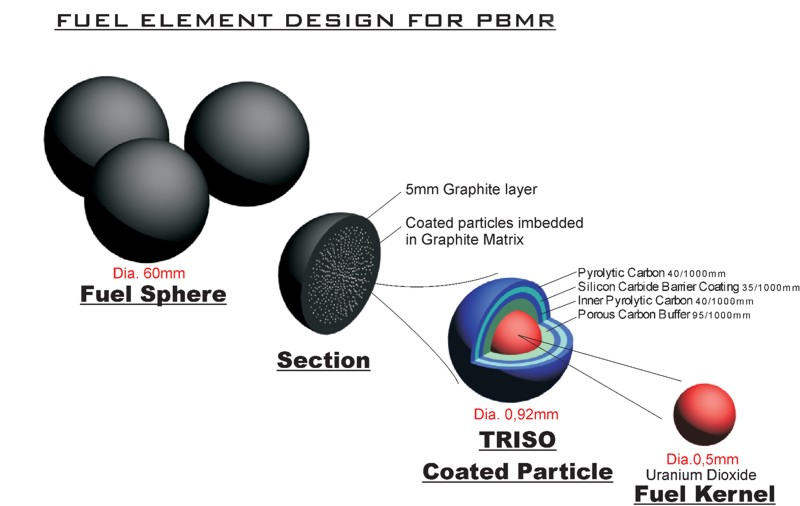
\includegraphics[width=0.85\textwidth]{./images/design/TMSR_fuel.jpg}
  \caption{Schematic of fuel pebbles and triso particles}
  \label{fig:triso}
\end{figure}

The question of how to model the complex geometry of the flow passage in a pebble bed has been tackled in chemistry engineering \cite{Dixon2001}\cite{Miroliaei2011} for fixed bed reactors in chemical processes and in nuclear engineering for pebble bed reactor designs.  The one-dimensional heat transfer simplification is often used in Light Water Reactor (LWR) fuel rods and can be used in spherical fuel elements for FHRs for quick scope analysis, but is inadequate for detailed investigation because it ignores temperature gradients in the axial and the radial direction, which can be significant in a FHR core with cross flow. Two main approaches for full core CFD modeling are realistic modeling and porous media modeling. Realistic modeling has been used to model flow passage directly in a segment of pebbles, from several to several hundreds \cite{Lee2007}\cite{Hassana}\cite{Shams2013}, but quickly becomes unfeasible for a large number of pebbles with the current computation resources. In addition, although the goal of realistic modeling is to model the flow passage realistically, it is not free of assumptions \cite{Lee2007}. For example pebble packing structure and contact point treatment are often used to reduce computational cost. The porous media approach, on the other hand, computes only the average flow conditions with ten time less mesh grids. Comparisons between the direct CFD and porous media methods\cite{Wu2010} suggest that porous media methods provide similar averaged pressure and temperature gradient across the pebble bed to the realistic approach, given the appropriate Darcy-Forchheimer drag model is used. Porous media approach has been used in standard HTR modeling tools Thermix \cite{Struth1985} and Tinte \cite{Gerwin1987}, as well as in a thermal-hydraulics model for FHR \cite{Scarlat2012}.
Appropriate safety margin should be applied in the design given the fact that porous media models do not capture local vertices, flow separation, variations in flow induced heat transfer around the pebble surface and the resulting local hot spots.

Previously, researchers have developed separate codes in thermal-hydraulics \cite{Scarlat2012} and neutronics \cite{Cisneros2013} for FHRs. These codes can be coupled for multiphysics computation using the operator-split method: solving one equation system at a time and transfer data between the codes after each iteration until the results converge. However, the operator split method requires small time steps to ensure convergence due to nonlinear inconsistency \cite{Ragusa2009} and could require a substantial amount of computational resource. This work, instead, explores methodology for developing fully coupled neutronics and thermal-hydraulics models for pebble bed FHRs.  


The rest of the paper is organized in three sections: the methodology, including governing equations, generation of cross-sections and implementation in COMSOL is discussed in section \ref{sec:methodology}; A case study based on TMSR design is then presented in section \ref{sec:res}, where model verification procedures via code-to-code comparison is presented and both steady state and transient results are discussed; Lastly, future research needs are identified and discussed in the conclusion.

\section{Methodology}
\label{sec:methodology}

\subsection{Neutronics}
\subsubsection{Multi-group neutron diffusion equations}
Multi-group diffusion equations, which provide a good balance between CPU cost and accuracy, is used in the multiphyscis model for neutronics computation. The governing equations of multi-group neutron diffusion with delayed neutrons are written as following:

\begin{align}
    \frac{1}{v_g}\frac{\partial \phi_g}{\partial t} = \nabla D_g \nabla \phi_g - \Sigma_{t,g}\phi_g + \sum_{g'=1}^{G} \Sigma_{s, g'g}\phi_{g'} +  \nonumber \\
    (1-\beta)\chi_{p,g}\sum_{g'=1}^G(\nu \Sigma_f)_{g'} \phi_{g'} + \chi_{d,g}\sum_{i=1}^D \lambda_iC_i
\label{eq:diffusion}
  \end{align}

\begin{equation}
    \frac{\partial C_i}{\partial t} = -\lambda_i C_i + \beta_i \sum_{g=1}^G (\nu \Sigma_f)_g \phi_g 
  \label{eq:delayed_neutrons}
\end{equation}
%
where the quantities are defined as follows:
\\
$v_g$ = neutron speed of the $g$-$th$ group, m/s
\\
  $\Sigma_{s, gg'}$ = macroscopic scattering cross-section from group $g'$ to group $g$, m$^{-1}$
\\
  $\nu$ = mean number of neutrons generated per fission
\\
$\Sigma_{f,g}$ = macroscopic fission cross-section of group $g$, m$^{-1}$
\\
  $\chi_g$ = fraction of delayed ($d$) or prompt ($p$) neutrons from fission generated in group $g$ 
\\
  $\phi_{g}$ = neutron flux in the $g$-$th$ energy interval [$E_g$, $E_{g-1}$], m$^{-2}$s$^{-1}$
\\
  %\begin{align}
  %  \phi_g(r,t) = \int^{E_{g-1}}_{E_g} \phi(r,E,t) dE
  %\end{align}
  $\Sigma_{t,g}$ = macroscopic total cross-section in group $g$, m$^{-1}$
\\
%  \begin{align}
%    \Sigma_{t,g} = \frac{1}{\phi_g}\int_g\Sigma_t(E)\phi(E)dE
%  \end{align}
%
  $D_g$ = diffusion coefficient for energy group $g$, m
\\
  $\beta_i$ = delayed neutron fraction for delayed neutron precursor group $i$
\\
  $\lambda_i$ = average decay constant of delayed neutron precursors, s$^{-1}$
\\
  $C_i$ = delayed neutron precursors concentration
 \\
 G = total number of energy groups\\
 D = total number of delayed neutron precursors groups.
  


For criticality calculations, the effective multiplication factor \keff is inserted into the neutron balance equation to represent the variation of neutron population from one generation to the following one.




\subsubsection{Cross-section generation}
The group-averaged, component-wise neutronic constants, used in the diffusion equations, are generated with the Monte Carlo neutron transport code Serpent using the nuclear data library ENDF/B-VII.0. 
In order to perform transient analysis, these cross-sections need to be paramatrized as functions of reactor operating conditions via a process called computer experiments, in which one runs a Monte Carlo model with a sample of operating conditions and fits a function between the resulting cross-sections and the input data.

The change in macroscopic cross-sections in the flibe region is mainly due to the change in density of liquid flibe with temperature, thus the function for flibe cross-sections are in the following form:

\begin{align}
  \hat{\Sigma}(\rho_{flibe}) = c_0 + c_1(\rho_{flibe} - \rho_0)
  \label{eq:flibe_xs}
\end{align}

where $\hat{\Sigma}(\rho_{flibe})$ is the estimation of a flibe macroscopic cross-section, $\rho_{flibe}$ is the flibe density that depends on the temperature, $\rho_0$ is the flibe density at nominal temperature, and 
$c_0$ and $c_1$ are the constants to be calculated.

Unlike liquid salt, the solid fuel elements do not change shape or density in the considered temperature range. 
The change in fuel cross-sections are mainly due to the Doppler broadening of the microscopic cross-sections of the fuel material and exhibit a linear-log function of temperature.  It is important for FHRs to compute the temperature distribution inside TRISO particles and fuel pebbles, and use the temperature profile, instead of an average fuel temperature, to compute cross-sections, because during fast transients such as reactivity induced accidents, the heat does not have time to propagate through the fuel pebbles and to reach the coolant and therefore the core relies on the temperature reactivity feedback inside the TRISO particles to stabilize.
A multiscale cross-section, incorporating a vector of temperatures at different depth in the fuel element, is express as a linear combination of the logarithm of fuel temperatures:

\begin{equation}
\hat{\Sigma} (T_{fuel}) = c_0 + [c_1, c_2, ... c_n] \begin{bmatrix}
    log(T_{11}) \\
    log(T_{12}) \\
    log(T_{13}) \\
    ...\\
    log(T_{nm})\\
\end{bmatrix}
\label{eq:linear_log}
\end{equation}


where $\hat{\Sigma}(T_{fuel})$ is the estimation of a macroscopic cross-section in the fuel region, $T_{fuel}$ is the temperature or temperature vector in case many temperatures affect the same cross-section, $T_{nm}$ is the temperature of the mth layer in a TRISO particle in the nth layer of a fuel pebble and $c_0$, $c_1$ are the coefficients we search for.

\subsection{Thermal-hydraulics}
Direct CFD modeling of the flow passage formed by more than 10000 pebbles is not practical with current computation capacity. The porous media approach, on the other hand, requires considerably less computational resource and is used in the multi-physics model.

An important parameter for porous media is the porosity, $\epsilon$, defined as the ratio between the volume of the void to the total volume (Equation \ref{eq:pf}). It appears in the mass (Equation \ref{eq:mass}), momentum (Equation \ref{eq:mmtm}) and energy conservation equations (equations \ref{eq:pm_liq} and \ref{eq:pm_sol}) below. Local variation in porosity in a pebble bed, including the drop near the wall due to ordered packing, is not modeled explicitly in the porous media model, but the empirical correlations for pressure loss and heat transfer coefficient incorporate corrections for wall effect.


\begin{equation}
  \epsilon = \frac{V_f}{V_f+V_s}
  \label{eq:pf}
\end{equation}

The mass conservation equation for the fluid phase in porous media is written as:
\begin{equation}
  \epsilon\frac{\partial \rho_f}{\partial t} + \nabla(\rho_fv) = 0
  \label{eq:mass}
\end{equation}

where $\rho_f$ is the fluid density in $kg.m^{-3}$, t time in s and v velocity vector in $m.s^{-1}$

The momentum equation for fluid flow in the pebble bed is written as:
% comsol
\begin{align}
  \frac{\rho_f}{\epsilon} \left[(u\nabla)\frac{u}{\epsilon} \right] + \rho\nabla u = &\nabla \left[ -pI + (\frac{\mu}{\epsilon}(\nabla u - (\nabla u)^T) - \frac{2\mu}{3\epsilon} \nabla u I)\right]  \nonumber\\
  &- (\frac{\mu}{k} + \beta_F \|u\| + \rho\nabla u) u + F
  \label{eq:mmtm}
\end{align}

The dependent variable here is the superficial velocity, the velocity that the fluid would flow if the channel is free of the solid medium. It is defined as the ratio between the volumetric flow rate and the effective cross section area of the flow channel (Equation \ref{eq:sv}).
\begin{equation}
  u=\frac{Q}{A}
  \label{eq:sv}
\end{equation}

Other parameters used in equation \ref{eq:mmtm} are:\\
$\rho_f$ = fluid density, kg/m3\\
$\epsilon$ = porosity\\
t = time, s\\
p = pressure, Pa\\
$\mu$ = dynamic viscosity, Pa.s\\
F = body force, $N/m^3$\\
I = identity matrix\\
K = permeability, $m^2$\\
$\beta_F$ = Forcheimer drag coefficient, $kg/m^4$\\

The Forcheimer drag coefficient $\beta_F$ and the permeability K are defined in the COMSOL momentum equation according to pebble bed pressure drop characteristics. 
Various pebble bed pressure drop correlations were investigated in previous studies \cite{Scarlat2012} and compared with experimental data \cite{Kang2010}. The most widely used is the Ergun correlation \cite{Ergun1949} for its wide range of validity in laminar, turbulent and transitional regions, its interpretability and convenient implementation, as well as the satisfactory results it provides. It models the pressure loss in a pebble bed as a weighted sum of the viscous energy loss and the inertial energy loss: 


\begin{equation}
  \frac{dp}{dx} = E_1 \frac{(1-\epsilon)^2\mu u}{\epsilon ^2 d^2} + E_2 \frac{1-\epsilon}{\epsilon^3}\frac{\rho u^2}{d}
  \label{eq:ergun}
\end{equation}



They are defined as in equation \ref{eq:betaf} and \ref{eq:K} so that the pressure drop equation in COMSOL (equation \ref{eq:comsol_dp}) matches the Ergun correlation (equation \ref{eq:ergun}).

\begin{equation}
  \frac{dp}{dx} = \frac{\mu}{K}u + \beta_F u^2
  \label{eq:comsol_dp}
\end{equation}

\begin{equation}
      K = \frac{1}{E_1}\frac{\epsilon^3 d^2}{(1-\epsilon)^2}
      \label{eq:K}
\end{equation}

\begin{align}
  \beta_F = c_F \frac{\rho}{\sqrt{K}}
  \label{eq:betaf}
\end{align}

where $c_F$ is the non-dimensional form of the Forcheimer drag coefficient that can be computed from Ergun correlation coefficients $E_1$ and $E_2$ as:

\begin{equation}
    c_F = \frac{E_2}{\epsilon^{1.5}\sqrt{E_1}}
\end{equation}



The energy equations for fluid and solid phases are given in equations \ref{eq:pm_liq} and \ref{eq:pm_sol}.
\begin{equation}
  \epsilon(\rho c_p)_f \frac{\partial T_f}{\partial t} + (\rho c_p)_f U\nabla T_f = \epsilon k_f \nabla\nabla T_f + \Phi + h_{sf}a(T_s - T_f)
  \label{eq:pm_liq}
\end{equation}

\begin{equation}
  (1-\epsilon)(\rho c_p)_s \frac{\partial T_s}{\partial t} =(1-\epsilon)k_s \nabla\nabla T_s + (1-\epsilon)q + h_{sf}a(T_f - T_s)
  \label{eq:pm_sol}
\end{equation}

In the energy equations, $\rho c_p$ is the volumetric heat capacity in $Jm^3K^{-1}$, $T_f$ and $T_s$ are respectively the fluid temperature and the solid temperature in K, $k_f$ is the fluid thermal conductivity in $Wm^{-1}K^{-1}$, a is the specific surface area in $m^{-1}$, q is the heat generation in $Wm^{-3}$.

In a typical nuclear reactor, 97\% of the energy is deposited in the fuel while the rest is transported in coolant, reflectors and even shield by long range particles such as neutrons and gammas. 
In the current model, nuclear power is assumed generated inside the solid medium of the fuel region and transferred to the coolant through heat convection. Reflectors have separate coolant channels to maintain the temperature and temperature in outer layers such as graphite reflectors and stainless steel containment has negligible effect on neutronics behaviour, therefore conservative adiabatic boundary condition is applied at the reflector walls and the temperatures of the outer layers are not computed in the coupled simulation. However, they can be computed using the coupled simulation results as boundary conditions.

In a porous media model, the convective heat transfer between the fuel pebbles and the coolant is computed from empirical correlations, whose validation affects directly the credibility of the results. The Wakao correlation (equation \ref{eq:wakao}) \cite{Wakao1979} calculates the convective heat transfer coefficient between pebbles and coolant, with Pr and Re the Prandtl and Reynolds numbers.

\begin{equation}
  Nu = 2 + 1.1 Pr^{1/3}Re^{0.6} 
  \label{eq:wakao}
\end{equation}

The convective heat transfer coefficient can be obtained from the Nussult number, the salt thermal conductivity k and pebble diameter $D_p$ using the relationship in equation \ref{eq:nuh}.

\begin{equation}
  h = \frac{kNu}{D_p}
  \label{eq:nuh}
\end{equation}


Inlet coolant temperature are imposed at the inlet boundary.  This enables modeling of overcooling transient by setting the inlet coolant temperature as a time dependent function. Either flow rate or detailed velocity profile perpendicular to the inlet surface can be imposed as flow straighteners are designed to make sure that the inlet flow is fully developed and the coolant injection channels are designed for prescribed inlet flow conditions.
Zero pressure is set to the outlet surfaces. Slip conditions neglect viscous effects are applied to the walls that contain the fluid.  

\subsubsection{Multi-scale temperature distribution}

In order to determine the temperature distribution inside fuel pebbles and TRISO particles, which is crucial for accurately determining the temperature reactivity feedback from the fuel material during transient scenarios, we use the 1-D heat diffusion equation in spherical coordinate to model the heat conduction inside solid fuel elements:

\begin{align}
  \rho C_p\frac{\partial T}{\partial t} = \frac{1}{r^2}\frac{\partial}{\partial r}\left(kr^2\frac{\partial T}{\partial r}\right) + g
\end{align}
where r is the radial coordinate of the point, $\rho$ is density, $C_p$ is specific heat capacity, T is temperature, t is time, k is thermal conductivity, and g is the heat generation density.

And the resulting equation from a change of variable $U(r,t)=rT(r,t)$ is shown below:

\begin{align}
  \frac{\partial U}{\partial t} = \alpha \frac{\partial ^2 U}{\partial r^2} + r \frac{g}{\rho C_p}
\end{align}

with boundary conditions:
\begin{align}
U_0 = 0\\
\frac{\partial U}{\partial r} |_{r=R} = \left( \frac{1}{R} - \frac{h}{k}\right) U + \frac{R}{k}hT_{\infty}
\end{align}

This equation system is readily solved numerically under finite volume discretization, where spherical elements, such as both fuel pebbles and TRISO particles, are divided into fine annuli, so that the temperature in each can be considered uniform. 
The resulting heat transfer equation for the jth layer in a TRISO particle that is situated in the ith layer of a fuel pebble is shown in equation \ref{eq:ij_diffusion}.

\begin{equation}
    \frac{\partial{Tp_{i,j}}}{\partial{t}}\rho_{i,j}c_{p_{i,j}} = \frac{k_{i,j}}{r_{i,j}}   \Bigg[  \frac {\frac{r_{i,j+1}T_{i,j+1}}{r_{i,j+1}-r_{i,j}}+\frac{r_{i,j-1}T_{i, j-1}}{r_{i,j}-r_ {i, j-1}  }}{\frac{1}{2}(r_ {i, j+1} -r_ {i, j-1} )}-\frac{2r_ {i, j} T_ {i,j} }{(r_ {i,j} -r_ {i,j-1} )(r_ {i, j+1} -r_ {i,j})} \Bigg]  + g  
    \label{eq:ij_diffusion}
\end{equation}

where r is the radius of TRISO particles.





\subsection{Implementation of the model and solver sequence}
\label{sec:implementation}

The model is implemented in COMSOL Multiphysics, a software package that solves systems of partial differential equations (PDEs) or ordinary differential equations (ODEs) using the Finite Element Method (FEM), by finding a solution composed of the sum of the product of shape functions and associated coefficients. 

After defining the geometry, input parameters and physics, the equation system is solved with a sequence of eigenvalue, steady state and time dependent solvers. 
It starts by searching for the eigenvalue of the neutronic system and the corresponding neutron flux and power distribution , with cross-sections computed from an initial guess of the temperatures. An eigenvalue solver evaluate the fluxes and power density values (Equation \ref{eq:powerdensity}) on an arbitrary scale, so the power density is normalized onto the operation power for the subsequent steady state solver, as shown in equation \ref{eq:scale}.  

\begin{equation}
  \dot{P} = \sum_{g=1}^G \kappa \Sigma_{f,g} \flux _g
  \label{eq:powerdensity}
\end{equation}

\begin{equation}
  \dot{P}_N = \frac{\dot{P}.P_{op}}{\iiint_V{\dot{P}dv}}
  \label{eq:scale}
\end{equation}

where the quantities are defined as follows:\\
$P_{op}$ = operation power, W\\
$\dot{p}$ = volumetric power density, $W/m^3$\\
$\dot{p}_N$ = normalized volumetric power density, $W/m^3$\\
$\kappa$ = mean energy generation per fission, $MeV$\\
$\Sigma_{f,g}$ = macroscopic fission cross-section of group $g$, m$^{-1}$\\
$\flux_{g}$ = neutron flux in the $g$-$th$ energy interval [$E_g$, $E_{g-1}$], m$^{-2}$s$^{-1}$\\
G = total number of energy groups.
 
Taking the neutron flux distribution found by the eigenvalue solver as an input, a stationary solver computes the temperature distribution in the core by solving the conservation equations in thermal-hydraulics modules. 

Another eigenvalue search is then performed with updated cross-section set based on the temperature distribution from the stationary solver. And the two steps are repeated until the results converge, i.e. the \keff differs by less than 1~pcm between two iterations.

At the end of the iteration, the fluxes are scaled so that the volume integration of the power density equals to the operating power of the reactor in simulation. Normalized delayed neutron precursor concentrations are also computed, from the normalized fluxes. The scaling factors for both are shown in the following equations:
\begin{equation}
    \flux_{gN} = \flux_g \frac{P_{op}}{\iiint_V{\dot{P}dv}}
\end{equation}

\begin{equation}
      C_{dN} = \frac{\beta_d \sum_{g=1}^G (\nu\Sigma_f)_g \flux_{gN}}{\lambda_d}\\
      = C_d\frac{P_{op}}{\iiint_V{\dot{P}dv}}
\end{equation}

where the quantities are defined as follows:\\
$P_{op}$ = operation power, W\\
$\dot{P}$ = volumetric power density, $W/m^3$\\
$\nu$ = mean number of neutrons generated per fission\\
$\Sigma_{f,g}$ = macroscopic fission cross-section of group $g$, m$^{-1}$\\
  $\flux_{g}$ = neutron flux in the $g$-$th$ energy interval [$E_g$, $E_{g-1}$], m$^{-2}$s$^{-1}$
\\
  $\beta_d$ = delayed neutron fraction for delayed neutron precursor group $d$
\\
  $\lambda_d$ = average decay constant of delayed neutron precursors in group d, s$^{-1}$
\\
  $C_d$ = delayed neutron precursors concentration in group d
 \\
 G = total number of energy groups\\
 D = total number of delayed neutron precursors groups.


Once the flux and neutron precursor concentration are scaled, one can simulate transient behaviour by solving the coupled equation system with time derivative terms in COMSOL's transient solver, with time step size being automatically chosen based on the time derivative of the dependent variables.



\section{Case study}
\label{sec:res}
The above methodolgoy is applied to a 10~MW research reactor design, the solid fuel Thorium Molten Salt Reactor (TMSR SF-1) \cite{wang2014a}, described in the following sections.

\subsection{TMSR SF-1 design overview}
As shown in Figure~\ref{fig:TMSR}, the TMSR SF-1 core measures 285~cm in diameter and 300~cm in height, and is composed with three major components: an upper region with fuel pebbles and flibe salt, a lower region with flibe salt and an outer graphite reflector region. Some key design parameters are listed in Table \ref{tab:tmsr_design}.

\begin{figure}[h]
    \centering
    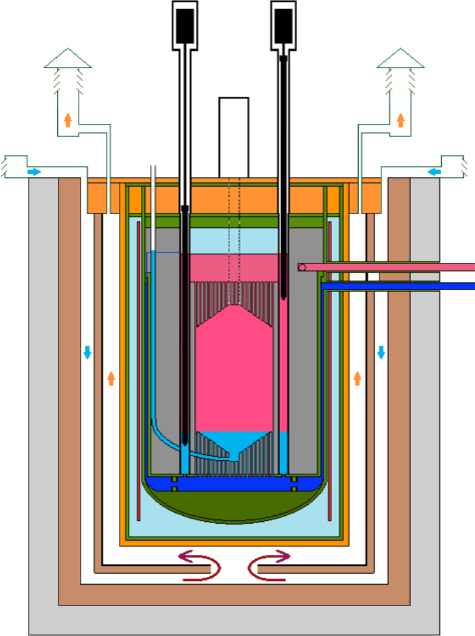
\includegraphics[width=0.6\columnwidth]{./images/design/TMSR_geom.png}
    \caption{Schematic of the TMSR core design and coolant path}
    \label{fig:TMSR}
\end{figure}

\begin{table}
  \centering
  \begin{tabular}{lc}
     \hline\\
     Parameter & Value \\
     \hline\\
     Nominal thermal power, MW & 10\\
     TRISO packing fraction & 9\% \\
     Uranium enrichment & 17.0\% \\
     Flibe Li-7 enrichment & 99.99\% \\
     Pebble diameter, cm & 6\\
     Approximate fuel pebble number& 11000\\
   Coolant inlet temperature, \degc& 672\\
   Coolant outlet temperature, \degc& 700\\
   Porosity & 40\% \\
   Fuel region radius, m& 0.68\\
   Coolant mass flow, kg/s & 150\\
   %Average coolant velocity, m/s & 0.14\\
   Height of the core (including reflector), m & 2.86\\
   Diameter of the core (including reflector), m & 2.6\\
   Control rods active length, m & 2.406\\
       %Convective heat transfer coefficient, $W/m^2K$&6000\\
     \hline\\
  \end{tabular}
  \caption{TMSR design parameters}
  \label{tab:tmsr_design}
\end{table}


TMSR SF-1 uses the same 6.0~cm fuel pebbles as those in the helium gas cooled high-temperature reactor (HTR), that contain a 5.0~mm thick graphite shell and the enclosed TRISO particles in a graphite matrix, as shown in figure \ref{fig:triso}. The dimension and material composition of the TMSR fuel element can be found in table \ref{tab:tmsr_pb}. As the figure also shows, the TRISO particles are made of multiple layers with detailed dimensions listed in table \ref{tab:tmsr_triso}. 
\begin{table}
  \begin{tabular}[h]{ccccc}
    Region&Material&Thickness/Radius&Density&Conductivity\\
    &&[mm]&[g/cc]&[W/m.k] \\
    \hline\\
    Shell&Graphite&1&10.5&3.5\\
    Fuel&TRISO+graphtie matrix&2&3.2&15\\
  \end{tabular}
  \caption{Dimensions and material properties of each layer of a fuel pebble}
  \label{tab:tmsr_pb}
\end{table}

\begin{table}
  \caption{Dimensions and material properties of each layer of TRISO particles.}
  \begin{tabular}[h]{lccccc}
    \hline
    Region&Material&Thickness,&Density,&Conductivity,&Specific heat,\\
    &&$10^{-6}$ m&kg/m$^3$&W/m/K&J/kg/K\\
    \hline
    Kernel&19.9\% UC$_{0.5}$O$_{1.5}$&250&10,500&3.5&400\\
    Buffer&porous carbon&95&1,000&0.5&2,000\\
    IPyC&pyrolytic carbon&40&1,900&4.0&2,000\\
    SiC&silicon carbide&35&3,200&30&1,300\\
    OPyC&pyrolytic carbon&40&1,900&4.0&2,000\\
    \hline
  \end{tabular}
  \label{tab:tmsr_triso}
\end{table}






TMSR SF-1 adopts a once-through fuel cycle, which although may not be the most economical approach comparing to online refueling, it is less demanding on the pebble handling system and is easier for predicting fuel composition in the core.
At the start of a fuel cycle, the pebbles are loaded individually from the bottom of the core into the flibe salt until the core reaches criticality, with about 11,000 fresh fuel pebbles. Fuel pebbles are buoyant in the salt and fills the upper region. The bottom of the fuel pebble bed has a cone shape with an angle depending on the pebble/fluid interaction. The lower region of the core is left with flibe salt.

The primary coolant (enriched liquid flibe) enters the core from the bottom at a nominal inlet temperature of 672\degc\ and flows upward across the pebble region with a nominal outlet temperature of coolant is 700\degc. The heat is then transported to the secondary loop through a heat exchanger for electricity production. 

The TMSR SF-1 core is surrounded by an outer graphite reflector, which provides neutron moderation and reflection that flattens the radial power distribution and improves neutron economy. It also hosts various channels for neutron sources, salt and pebble loading and instrumentation, as well as the 16 control rods for reactivity control.


\subsection{Multiphysics modeling for TMSR SF-1}

As shown in Figure \ref{fig:model_geom}, the multi-physics reactor core model is composed by three regions: an upper porous region that represents a fuel pebble and flibe salt porous mixture, a lower region with only flibe salt and an outer graphite reflector region. Coupled heat transfer and neutron diffusion equations are solved with homogenized material properties for each region. 


\begin{figure}[h]
  \centering
  \begin{subfigure}{0.2\textwidth}
    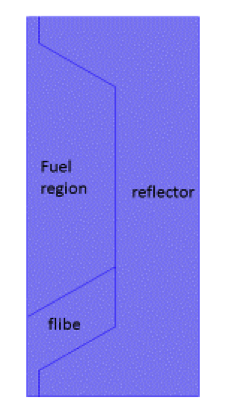
\includegraphics[width = \columnwidth]{./images/diffusion/tmsr/2d_schematic.png}
    %\caption{Schematic of the TMSR core model geometry}
  \end{subfigure}
  ~
  \begin{subfigure}{0.55\textwidth}
    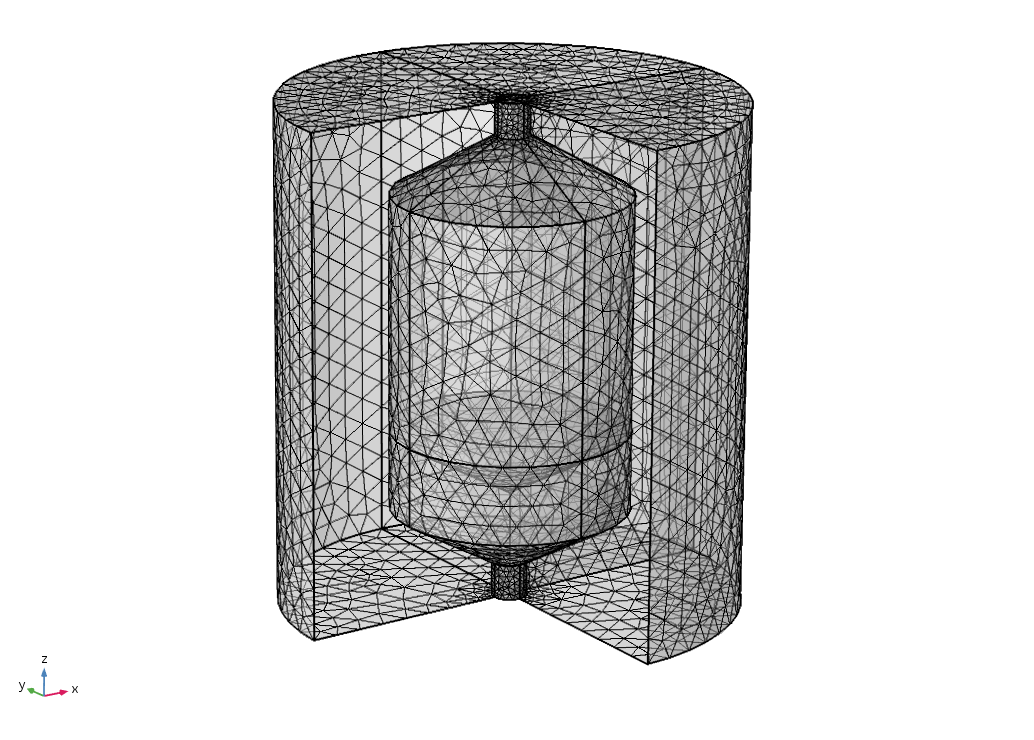
\includegraphics[width = \columnwidth]{./images/diffusion/tmsr/finer.png}
    %\caption{Schematic of the 2D mesh}
  \end{subfigure}
  \caption{Schematic of the multi-physics model for TMSR SF-1 and a three-dimensional mesh}
  \label{fig:model_geom}
\end{figure}

Multigroup neutron diffusion equations are implemented into COMSOL as user defined PDEs, with the homogenized group constants for each regions defined as input. 
The group constants that are used by the diffusion and $SP_N$ models are generated from a Serpent model for the TMSR SF-1 core with explicit representation of randomly packed TRISO particles and fuel pebbles, with the locations given by Discrete Element Method(DEM) computation, although studies\cite{Fratoni2007} have shown that the packing configuration does not affect the results, provided the packing fraction is preserved when pebbles near the wall are cut arbitrarily by the geometry definition. 

In order to automate the process and to ensure reproducibility of the results, a MATLAB code is developed to read data from Serpent output files, fit the parameters to the respective functions of reactor conditions, and input the group constants into COMSOL. The code is set up for any user defined group structures and the one that is used in the current models is shown in table \ref{tab:egroup}. The eight-group energy structure is chosen to capture the cross section features of the major isotopes: U-235, U-238, and those in flibe. Figure \ref{fig:xs_isotope} shows the normalized spectrum in different reactor zones and the scattering, fission, absorption and (n, 2n) cross sections of the major isotopes, in superposition of the currently used group structure. 

\begin{figure}[h]
  \centering
  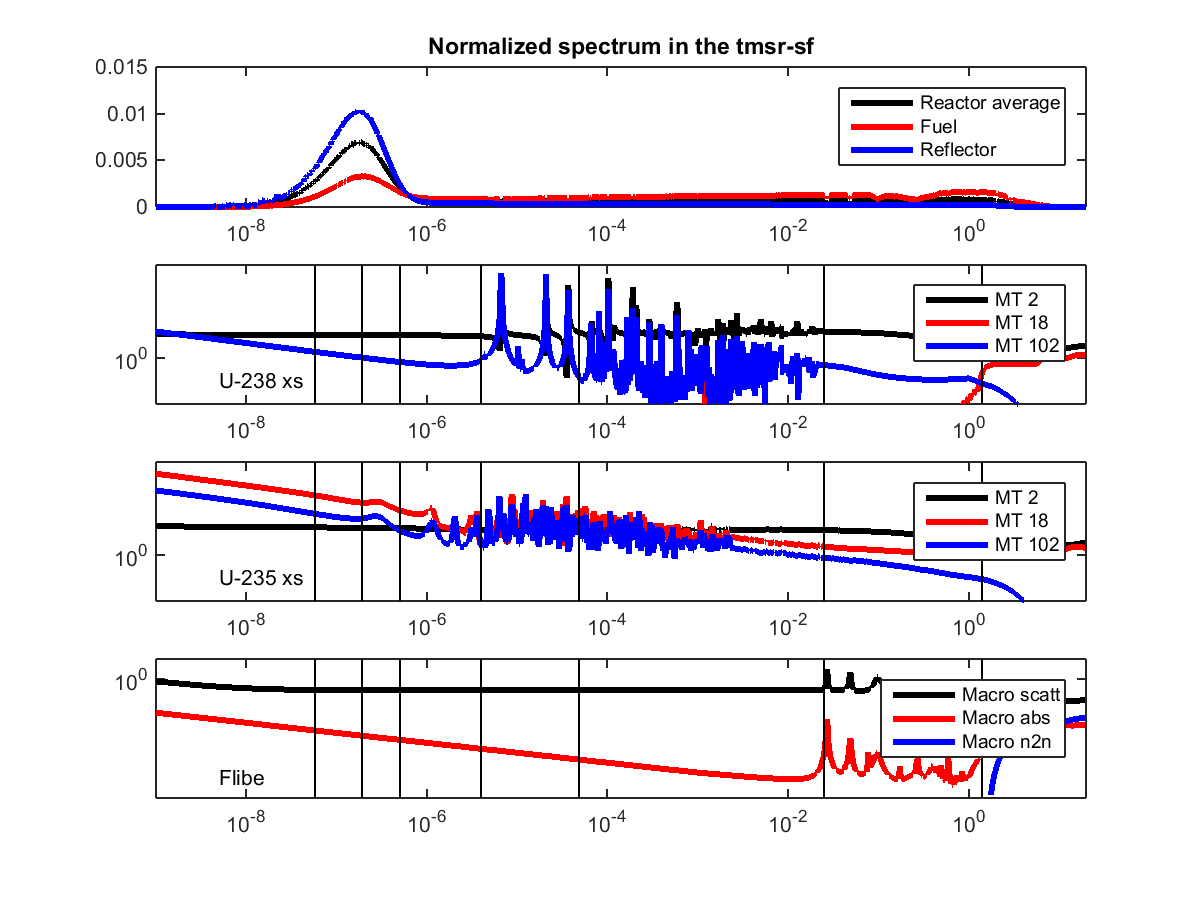
\includegraphics[width=0.8\textwidth]{./images/diffusion/tmsr/isotope_XS.png}
  \caption{Cross sections of major isotopes in the core.}
  \label{fig:xs_isotope}
\end{figure}

\begin{table}
\caption{Energy group structure adopted in the multi-group neutron diffusion model.}
  \centering
  \begin{tabular}{cc}
  Group \# & Upper energy bound, MeV\\
  \hline
  1 & 20.E+00\\
  2 & 1.4E+00\\
  3 & 2.5E-02\\
  4 & 4.8E-05\\
  5 & 4.0E-06\\
  6 & 5.0E-07\\
  7 & 1.9E-07\\
  8 & 5.8E-08\\
  \hline
  \end{tabular}
  \label{tab:egroup}
\end{table}

The thermal-hydraulics model is implemented in COMSOL as well, so that the multiphysics equation system can be solved in a fully coupled fashion. 
The model uses thermal property values in Table \ref{tab:flibe} for flibe coolant and graphite reflector. The homogenized pebble-wise properties and the properties of each layer of the fuel elements are listed in Table \ref{tab:TRISO_prop} and Table \ref{tab:pb_prop}. These nominal values are used in most of the models where the variation in thermo-physical properties for solid materials are not significant within the range of the temperature change. 



\begin{table}
  \caption{Flibe salt thermo-physical properties.}
  \centering
  \begin{tabular}{lc}
    \hline
    Property & Value\\
    \hline
    Viscosity, kg/m.s & 1.16E-4*e$^{3755/T[K]}$\\
    Heat capacity, J/kg/K & 2386\\
    Thermal conductivity, W/m/K & 1.1\\
    Density, kg/m$^3$ & 2413 - 0.488T[K]\\
    \hline
  \end{tabular}
\label{tab:flibe}
\end{table}


To model the flow field and heat transfer in the pebble bed, porous media approach computes a liquid temperature and a fuel temperature at each point in the region and connect the two phases through convective heat transfer. The fuel temperature is of prime important in FHR transient response because of the large Doppler temperature reactivity feedback. Therefore, multiscale temperature treatment is implemented for a more realistic representation of the feedback from fuel temperature changes. 

Temperature inside fuel pebbles are computed in three subdivided fuel layers, and likewise the fuel kernel in the TRISO particles are divided into three sub-layers, for which temperatures are tracked during a transient and are used to compute fuel region macroscopic cross-sections. In order to save computational cost, the coatings are combined into a non-heat-generating layer with equivalent heat transfer properties. The effects of this treatment on the response to reactivity insertion and overcooling transients are discussed further in section \ref{sec:TMSR_transients} when we analyze the TMSR transient behaviors.

A vacuum boundary condition is applied at the outer surfaces of the reflector. And a symmetry boundary condition is used at the core center-line in 2-D axi-symmetrical models.




% ----------------------------------------------------------------------------------------------------------------------
\subsection{Mesh refinement study}
he TMSR core model with homogenized regions is meshed with free triangular (2D) or tetrahedral (3D) elements. The effect of mesh size on solution accuracy is studied through mesh refinement studies, where the mesh element size is decreased gradually, with the minimum mesh size ranging from 0.1 m to 0.004 m, and the solutions are compared. 

\begin{figure}
\centering
    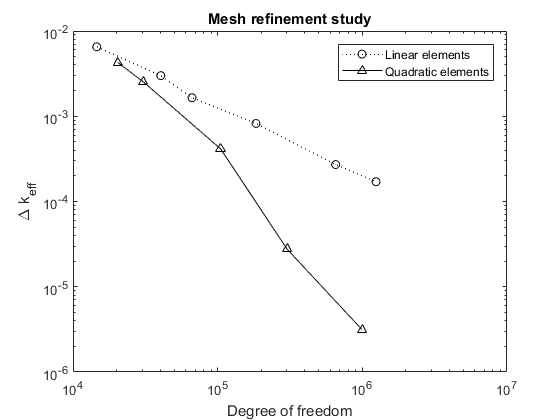
\includegraphics[width = 0.8\textwidth]{./images/diffusion/tmsr/mesh_refinement.png}  
    \caption{Logarithmic decrease in computation error with increase in degree of freedom for both linear elements and quadratic elements}
    \label{fig:mesh_refinement}
\end{figure}

Figure \ref{fig:mesh_refinement} shows the difference in the multiplication factor between a given mesh and the reference. Both quadratic and linear elements are studied. The finest quadratic mesh is used as reference. The plot shows an almost exponential trend between degree of freedom and the computation error. 
Also shown on the plot is that the order of the polynomial functions defined over the mesh elements affects the speed at which the solution converges. This is because FEM method solves the equations by finding a solution composed of the sum of the product of shape functions and associated coefficients. Higher order functions represent the solution with larger flexibility and can approximated the real solution with less elements. 
 
Finer mesh provides more accurate results but also requires more computer resources. One needs to choose the mesh size by balancing the available resource and desirable accuracy. 




\subsection{Model verification}
Code-to-code comparison is crucial for code verification when experimental data is lacking. Code verification has been done in this work by comparing both steady state and time dependent results to a reference code under various conditions. 

The reference model \cite{Aufiero2016} uses Serpent for neutron transport and OpenFOAM for CFD modeling. These two codes are internally coupled for best computation performance. To model the reactor core as realistic as possible, the random packing of TRISO particles and fuel pebbles are also simulated, using discrete element method (DEM). The reference model can computes three dimensional distribution of power, temperature, neutron flux, as well as global parameters such as $k_{eff}$, temperature reactivity feedback coefficients. 
Serpent solves the neutron transport equation in integral form using continuous energy nuclear data with few approximations, therefore it produces valuable reference results for code-to-code verification where experimental data are not available. 

\subsubsection{Power distribution comparison}
\begin{figure}
  \centering
  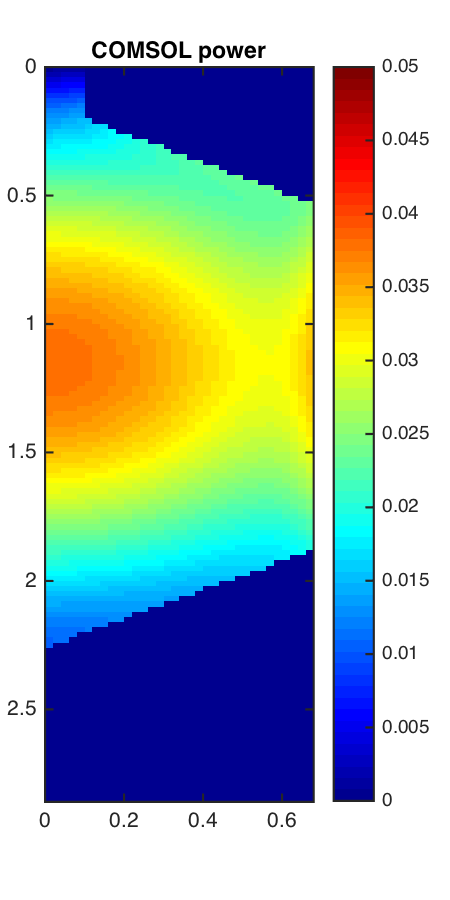
\includegraphics[width=0.35\columnwidth]{./images/benchmark/comsol_power.png}
  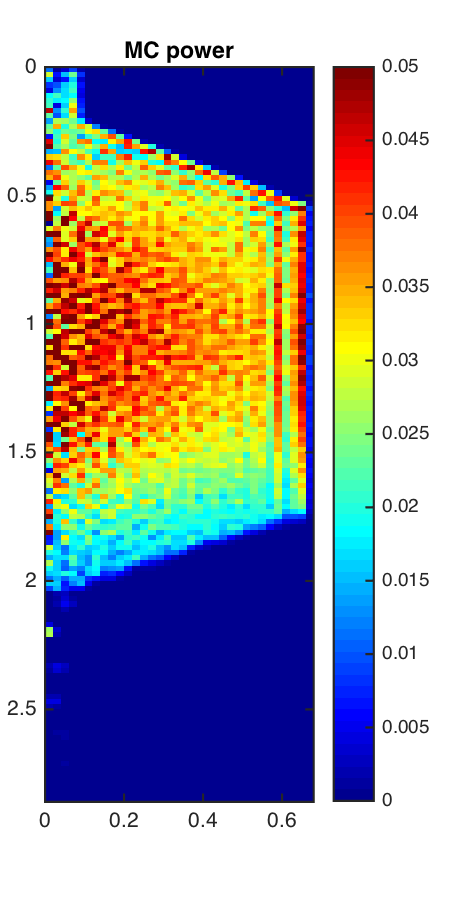
\includegraphics[width = 0.35\columnwidth]{./images/benchmark/MC_power.png}
  \caption{Steady state power profile computed from the COMSOL model and the Monte Carlo reference model}
  \label{fig:power_comp}
\end{figure}

Isothermal condition, whereby the core is maintained at uniform temperature by external heat source, is a good starting point for code-to-code comparison for the neutronic modules as they do not require coupling with thermal-hydraulics. In order to verify the reliability of the neutronic modules, the power density distribution is computed.


Figure \ref{fig:power_comp} shows the steady state power distribution on a 2.0~cm x 2.0~cm mesh, the result from the COMSOL model on the left and that from the reference model on the right, both normalized such that the full core integration is unity. 
Satisfying similarity has been found between the results. The diffusion-based model captures the boundary effect of the reflector adequately despite the fundamental flaw of the diffusion assumption in vicinity of the boundaries. However, because the individual pebbles are not explicitly modeled, the diffusion model cannot represent the local variation in power due to the discrete packing of fuel pebbles. As a result, the power profile seems smoother in the COMSOL model. 
In a randomly packed pebble bed, the porosity is slightly higher at the center and lower at the wall because of the ordering effect. Near the walls, the Monte Carlo result shows a drop in power density due to ordered pattern of pebbles, but this can not be captured by the COMSOL model because it uses homogenized cross sections in the fuel region. The variation can be better reflected in the COMSOL model if the core is divided into multiple radial zones, with different set of cross-sections generated for each zone.
Furthermore, the interface between the fuel pebble region and the flibe region is approximated by a straight line in the COMSOL model. This is different from the randomly packed fuel region in the reference model but can be calibrated for a better match. 


% \begin{figure}[ht]
%   \centering
%   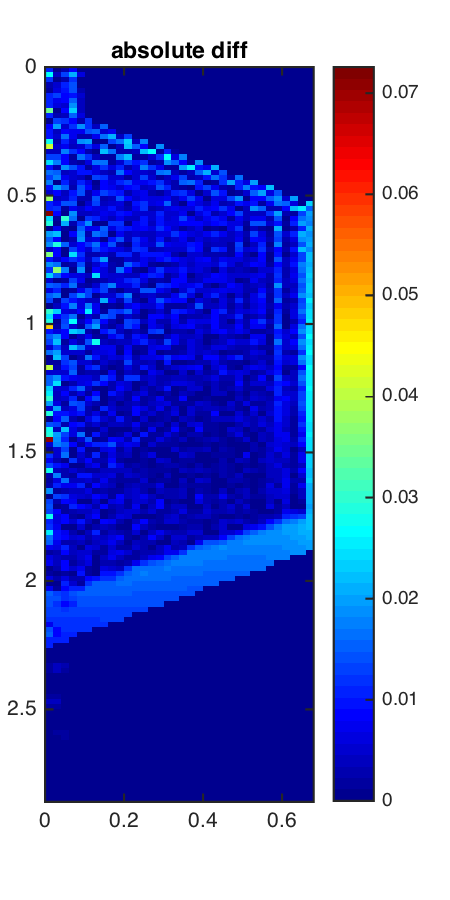
\includegraphics[width=0.3\columnwidth]{./images/benchmark/diff_abs.png}
%   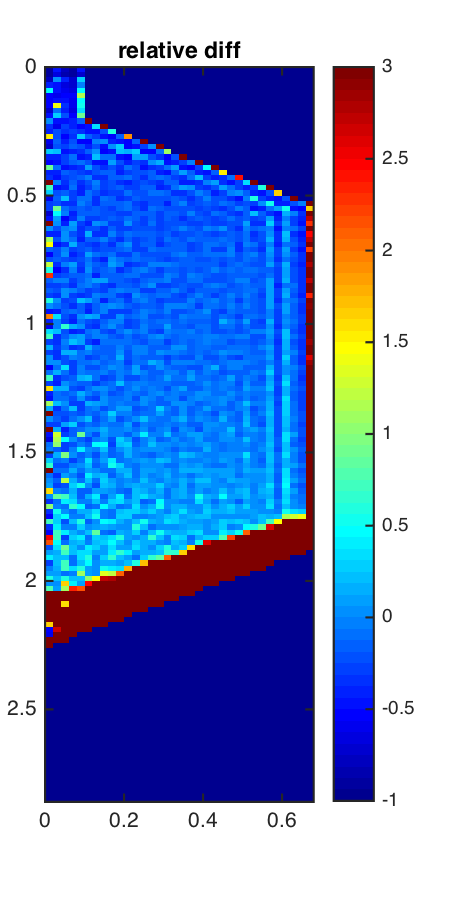
\includegraphics[width = 0.3\columnwidth]{./images/benchmark/diff_rel.png}
%   \caption{Steady state power profile computed from the COMSOL model and the Monte Carlo reference model}
%   \label{fig:power_comp_diff}
% \end{figure}

\begin{figure}
  \centering
  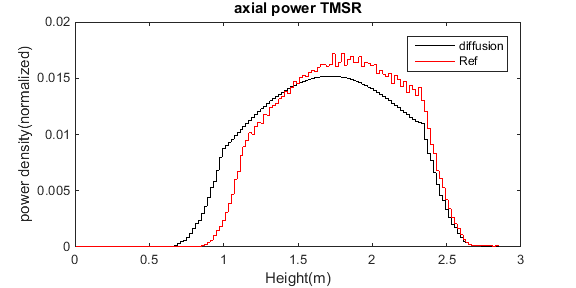
\includegraphics[width=0.7\columnwidth]{./images/benchmark/axial_TMSR.png}
  \caption{Comparison of the axial distribution of normalized power}
  \label{fig:axial_power}
\end{figure}

\begin{figure}
  \centering
  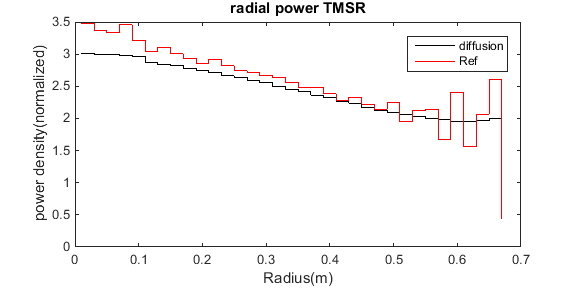
\includegraphics[width=0.7\columnwidth]{./images/benchmark/radial_TMSR.png}
  \caption{Comparison of the radial distribution of normalized power}
  \label{fig:radial_power}
\end{figure}

In addition to the qualitative comparison of the two-dimensional (r, z) profiles, the power density is integrated along the axial or radial directions and the resulting axial or radial power distributions are compared respectively in figure \ref{fig:axial_power} and \ref{fig:radial_power}. 
The difference in axial power from the two codes in figure \ref{fig:axial_power} is mainly due to the approximation in the shape of the fuel region that the COMSOL model makes. The most obvious discrepancy is found at the fuel-flibe interface, where the power density drops to zero, but this can be better calibrated in the geometry.
Figure \ref{fig:radial_power} shows the difference in radial power distribution. The step changes in power density along the radius in the reference result is due to the effect of discrete pebble packing, which causes local variations in fuel pebble packing fraction. This phenomena is not captured in the COMSOL model.





\subsection{Multiplication factor comparison}
The first global parameter that is compared under isothermal conditions is the multiplication factor, which is the most important global parameter in nuclear reactor modeling and control. 
At the same nominal conditions (flibe density at 1.9~$g/cm^3$ and fuel temperature at 900~K), the multiplication factor value from COMSOL and reference model is shown in table \ref{tab:keff}. The difference between the COMSOL model and the reference model is larger than two times of the Monte Carlo statistical error, indicating that the difference is statistically significant. This shows that diffusion based models are inadequate in computing the neutron multiplication factor. 

However, for transient analysis, which we are most interested in, the changes in the multiplication factor when the operation conditions deviates from the nominal ones is more important than the absolute values.
And the time scale and amplitude of these changes are compared respectively in section \ref{sec:time_scale} and section \ref{sec:feedback}.

%1051K for flibe
\begin{table}
\centering
  \begin{tabular}{lc}
  \hline
        Parameter & value \\
        \hline\\
       COMSOL \keff & 1.03029  \\
       Reference \keff & 1.08416$\pm$ 0.00012\\
       $\Delta$\keff & 0.05397\\
       %Reference statistical error & 0.00012\\
       \hline
  \end{tabular}
  \caption{Comparison of multiplication factor}
  \label{tab:keff}
\end{table}






\subsection{Time constant comparison}
\label{sec:time_scale}

\begin{figure}[h]
  \centering
  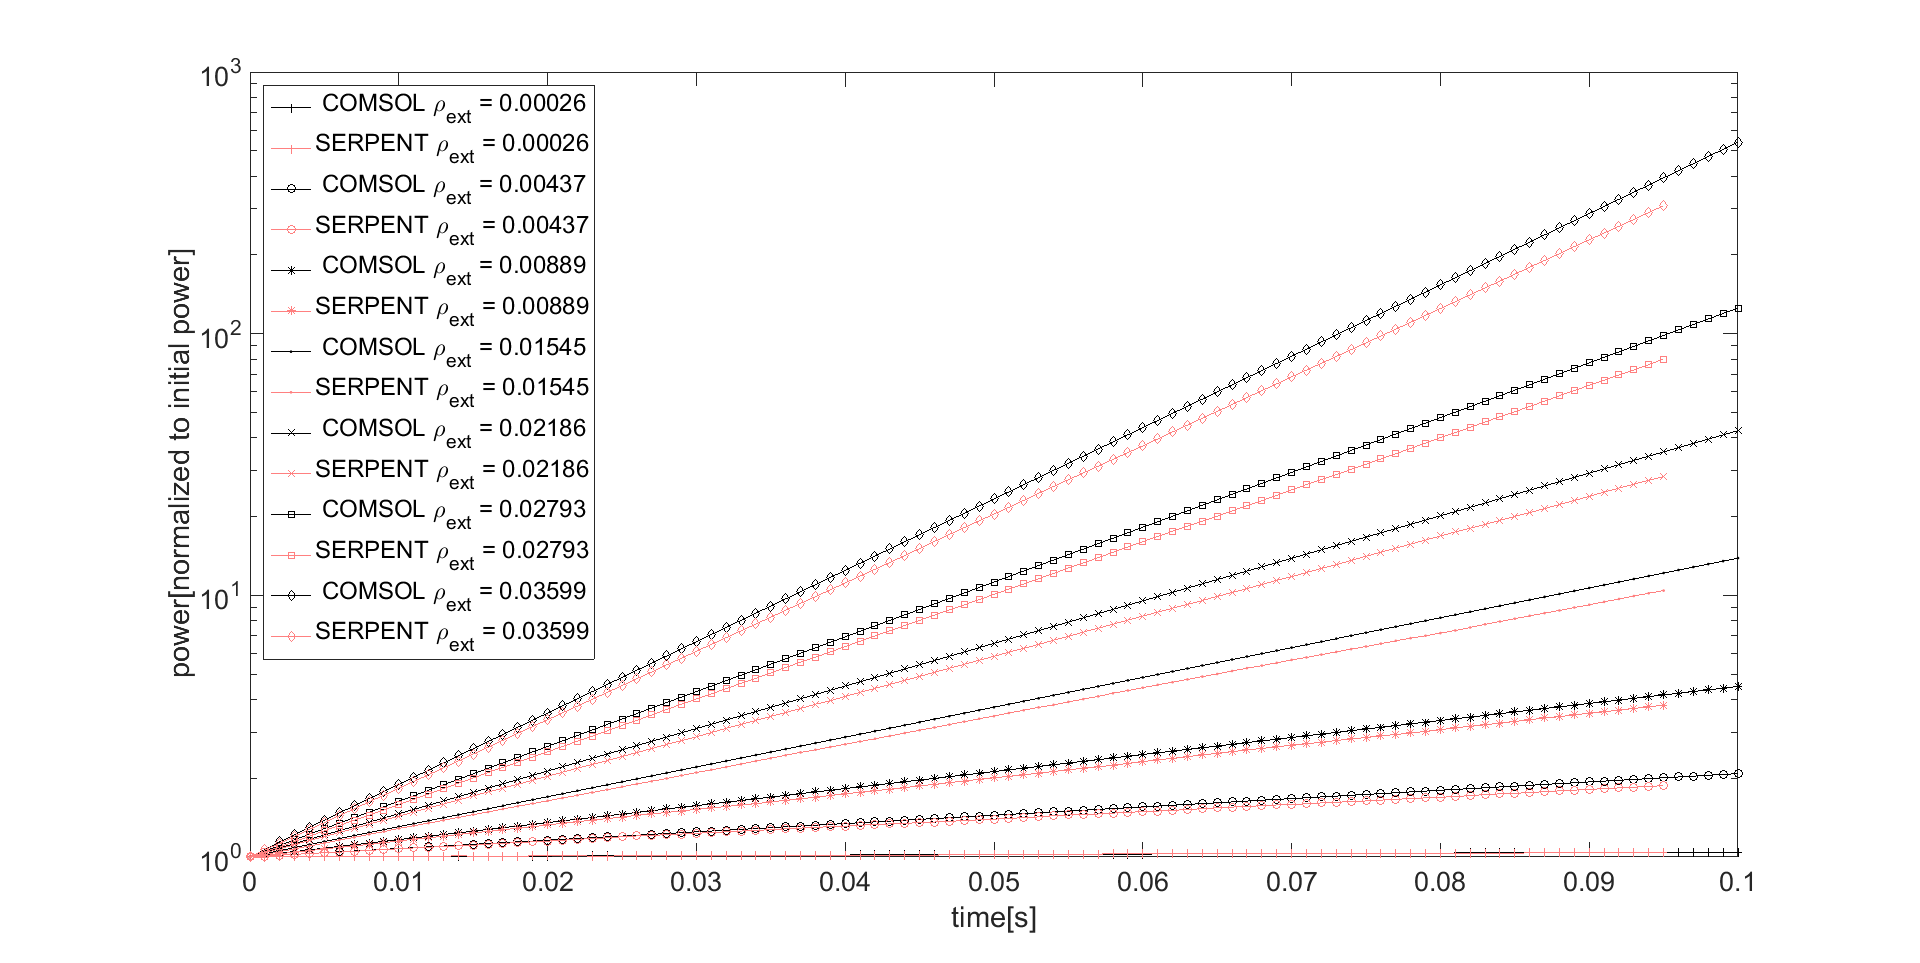
\includegraphics[width=\columnwidth]{./images/benchmark/zero_power_transient.png}
  \caption{Comparison between the diffusion based model and the Monte Carlo based model for zero power reactivity insertion transients}
  \label{fig:zero_power}
\end{figure}

The time constant of the system is compared via zero power reactivity insertion transient simulations. External reactivity is inserted into the core at norminal zero power conditions and without temperature reactivity feedback that would stablize the power at a certain level, the reactor power increases exponentially due to excess external reactivity, as shown in Equation \ref{eq:pexp}. 
The speed in which the power ramps up is a direct characteristic of the reactor time scale in the model, as shown in equation \ref{eq:pexp}. 

\begin{equation}
P/P_0 =  e^{\rho t/\lambda}
\label{eq:pexp}
\end{equation}
where P is the real time power, $P_0$ is the initial power, $\rho$ is the reactivity, t is time, and $\lambda$ is the characteristic time constant of the system. 

Figure \ref{fig:zero_power} shows the power excursion within 0.1 second following a reactivity insertion.
As we can see, the results from the COMSOL model match closely to those from the Serpent model, as well as the analytical prediction, for a large range of inserted reactivities, from 26 pcm to 3599 pcm.  






\subsection{Temperature feedback comparison}
\label{sec:feedback}

\begin{figure}
  \centering
  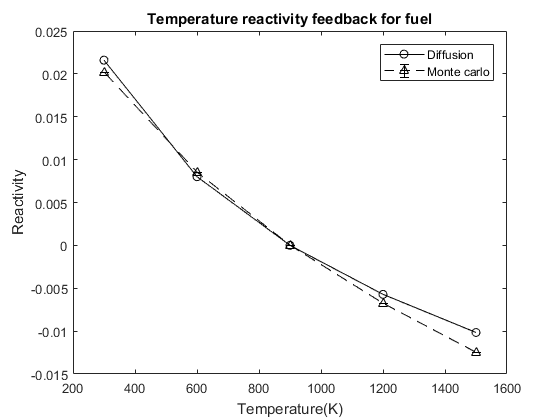
\includegraphics[width=0.6\columnwidth]{./images/benchmark/feedback_fuel.png}
  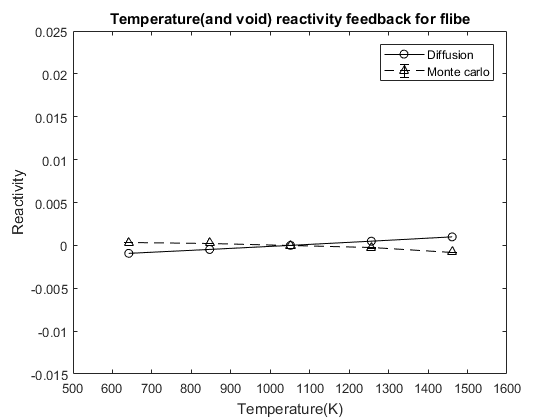
\includegraphics[width=0.6\columnwidth]{./images/benchmark/feedback_flibe.png}
  \caption{Comparison between the diffusion based model and the Monte Carlo based model for fuel and flibe temperature (and void) feedback effect. Error bar shows statistical error in Monte Carlo results.} 
  \label{fig:fuel_feedback}
\end{figure}



The ability of accurately capturing the temperature reactivity feedback coefficients is crucial for a coupled neutronics and thermal-hydraulics model because these parameters are the macroscopic manifestation of the coupling between thermal hydraulics and neutronics. They embody the effects of temperature change on core neutronics. 

The two major ones in FHR, the fuel Doppler feedback and the coolant temperature feedback coefficients, are computed from both models and are compared in figure \ref{fig:fuel_feedback}. The same y-axis range is used in the two plots for a visual comparison of the order of magnitude of these two feedback mechanisms. The fuel Doppler feedback is obviously the dominant effect in TMSR SF-1 cores.

To calculate the temperature reactivity coefficients, the temperature of the fuel component is varied by 300 K in the range between 300 K and 1500 K and the density of the flibe is changed by 100 $kg/m^3$ between 1700 $kg/m^3$ and 2100 $kg/m^3$. The coolant temperature reactivity coefficient includes the effect of temperature on cross sections, as well as the effect of density change due to temperature. 
In order to compare the variation of reactivity due to temperature change, delta reactivity is compared. It is computed as the difference between the reactivity at a reference temperature (900K for fuel and 1051K for flibe, which corresponds to a density of 1900 $kg/m^3$) and at a given temperature. 


The fuel temperature feedback curves agree well. 
The relative error in flibe reactivity feedback is larger but the absolute error is small due to the small magnitude of flibe feedback. And the discrepancy between flibe feedbacks is within statistical errors of the Monte Carlo computation. 


\subsection{Steady state results}
After careful code-to-code verification for the multi-physics model, parameters such as power, flibe and fuel temperatures, and neutron flux are computed. Uniform temperature and uniform upward velocity are imposed as the inlet boundary condition. Vacuum boundary condition for neutron diffusion is used outside of the reflector.  

% flux
\begin{figure}
  \centering
  \begin{subfigure}[b]{0.46\textwidth}
        \centering
        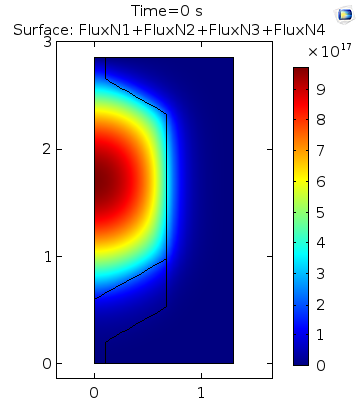
\includegraphics[width=0.9\textwidth]{./images/diffusion/tmsr/SS/non_ms/fast_flux.png}
        \caption{Fast neutron flux ([5.00E-07, 1.40] MeV)}
    \end{subfigure}%
    ~
    \begin{subfigure}[b]{0.46\textwidth}
        \centering
        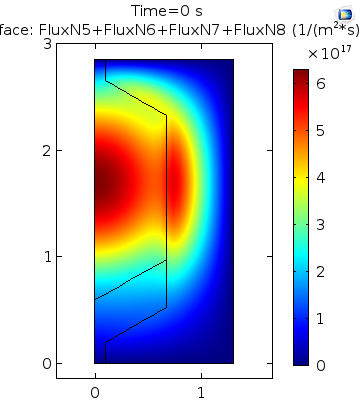
\includegraphics[width=0.9\textwidth]{./images/diffusion/tmsr/SS/non_ms/thermal_flux.png}
        \caption{Thermal neutron flux ([0.00, 5.00E-07] MeV)}
    \end{subfigure}
    \caption{Steady state neutron flux}
    \label{fig:ss_res_flux}
\end{figure}

An eight-group energy structure is used in the neutron diffusion equations but the neutron flux values are regrouped into thermal ([0.00E+00, 5.00E-07] MeV) and fast ([5.00E-07, 1.40E+00] MeV) regions for plotting purpose. As confirmed by the plots, fast neutrons are generated exclusively from nuclear reactions in the fuel region and are then scattered by the matters in the core as they get thermalized. 
The moderation effect of the coolant is dwarfed by that of the graphite reflector in TMSR. As a result, a large portion of thermal neutrons is found inside the reflector, besides the center of the core.

The thermal neutrons that travel back from the reflector to the fuel region cause a peak in power density near the border as they trigger nuclear reactions. 

% power
\begin{figure}
    
        \begin{subfigure}{0.45\textwidth}
        \centering
        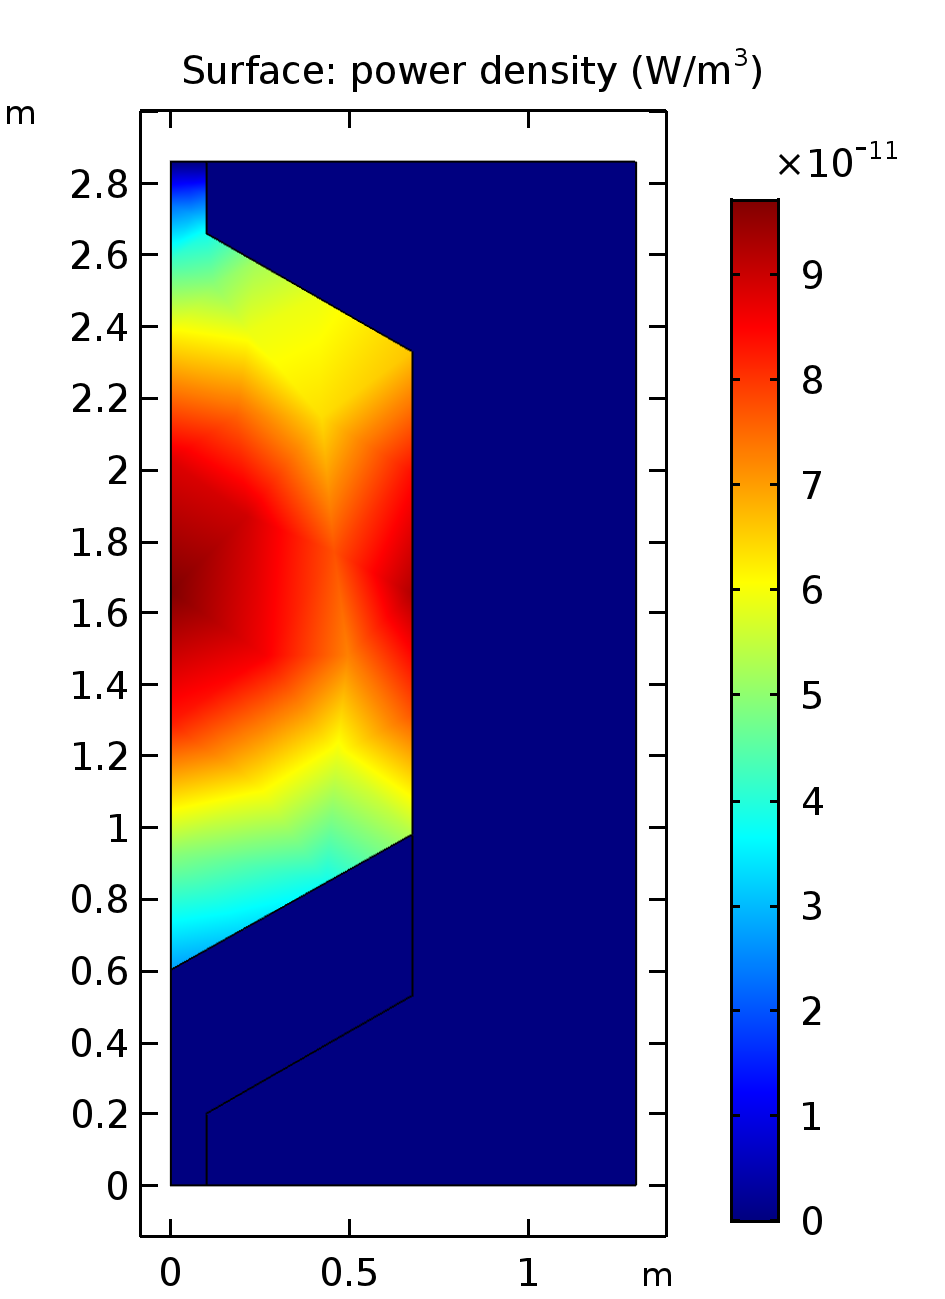
\includegraphics[width=0.8\textwidth]{./images/diffusion/tmsr/SS/non_ms/Pdensity(steady_state).png}
        \end{subfigure}
        ~
        \begin{subfigure}{0.5\textwidth}
        \centering
        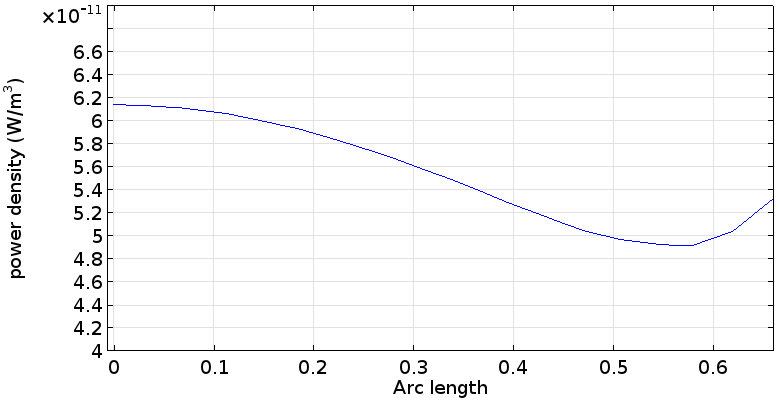
\includegraphics[width=0.8\textwidth]{./images/diffusion/tmsr/SS/non_ms/power_peaking_r.png}
        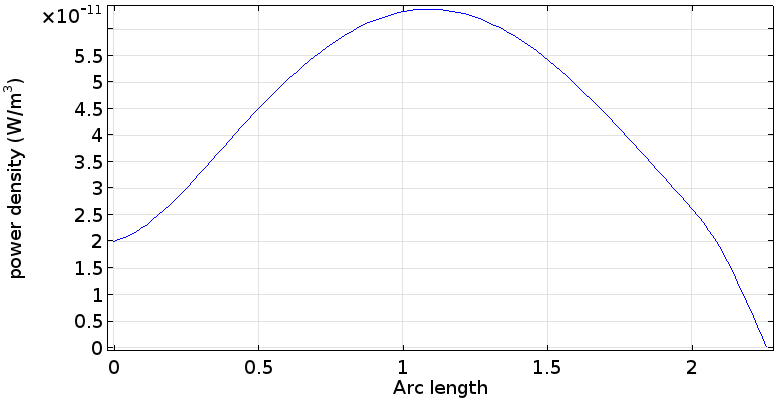
\includegraphics[width=0.8\textwidth]{./images/diffusion/tmsr/SS/non_ms/power_peaking_z.png}
        \caption*{Radial and axial power profile}
    \end{subfigure}%
    
    \caption{Power distribution in TMSR SF-1}
    \label{fig:tmsr_power_ss}
\end{figure}

As shown in figure \ref{fig:tmsr_power_ss}, the power peaks at the center of the fuel region, decreases outward and increases again next to the reflector boundaries due to the moderation effect of the graphite reflector. This confirms that the neutron diffusion based model captures the boundary effect adequately. The radial power peaking in TMSR SF-1 is 1.24 at nominal conditions with fresh fuel.

 

\begin{figure}[h]
  \centering
    \begin{subfigure}[b]{0.3\textwidth}
        \centering
        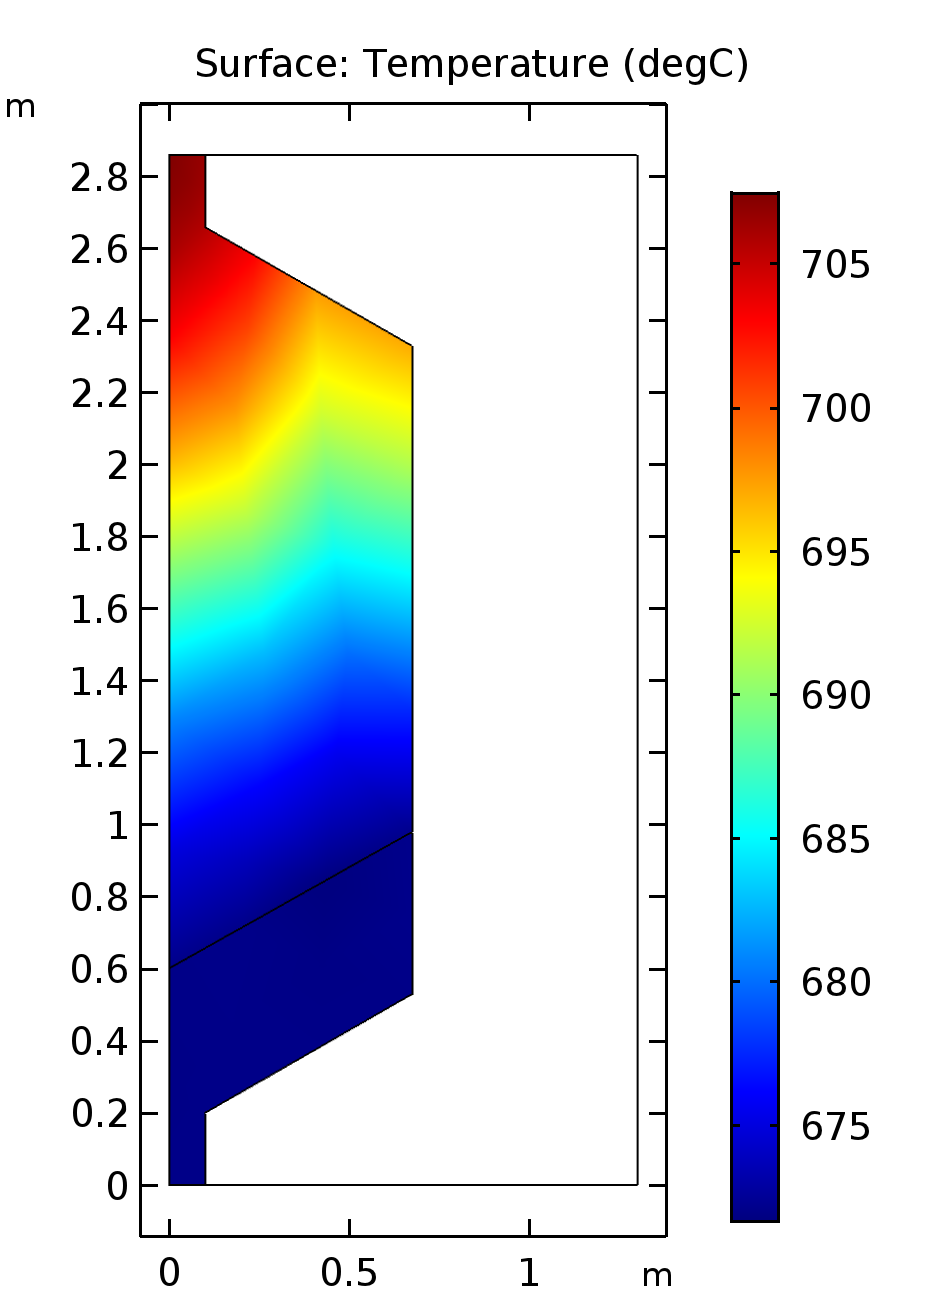
\includegraphics[width=0.9\textwidth]{./images/diffusion/tmsr/SS/non_ms/T_flibe(steady_state).png}
        \caption{Flibe}
    \end{subfigure}%
    ~
    \begin{subfigure}[b]{0.3\textwidth}
        \centering
        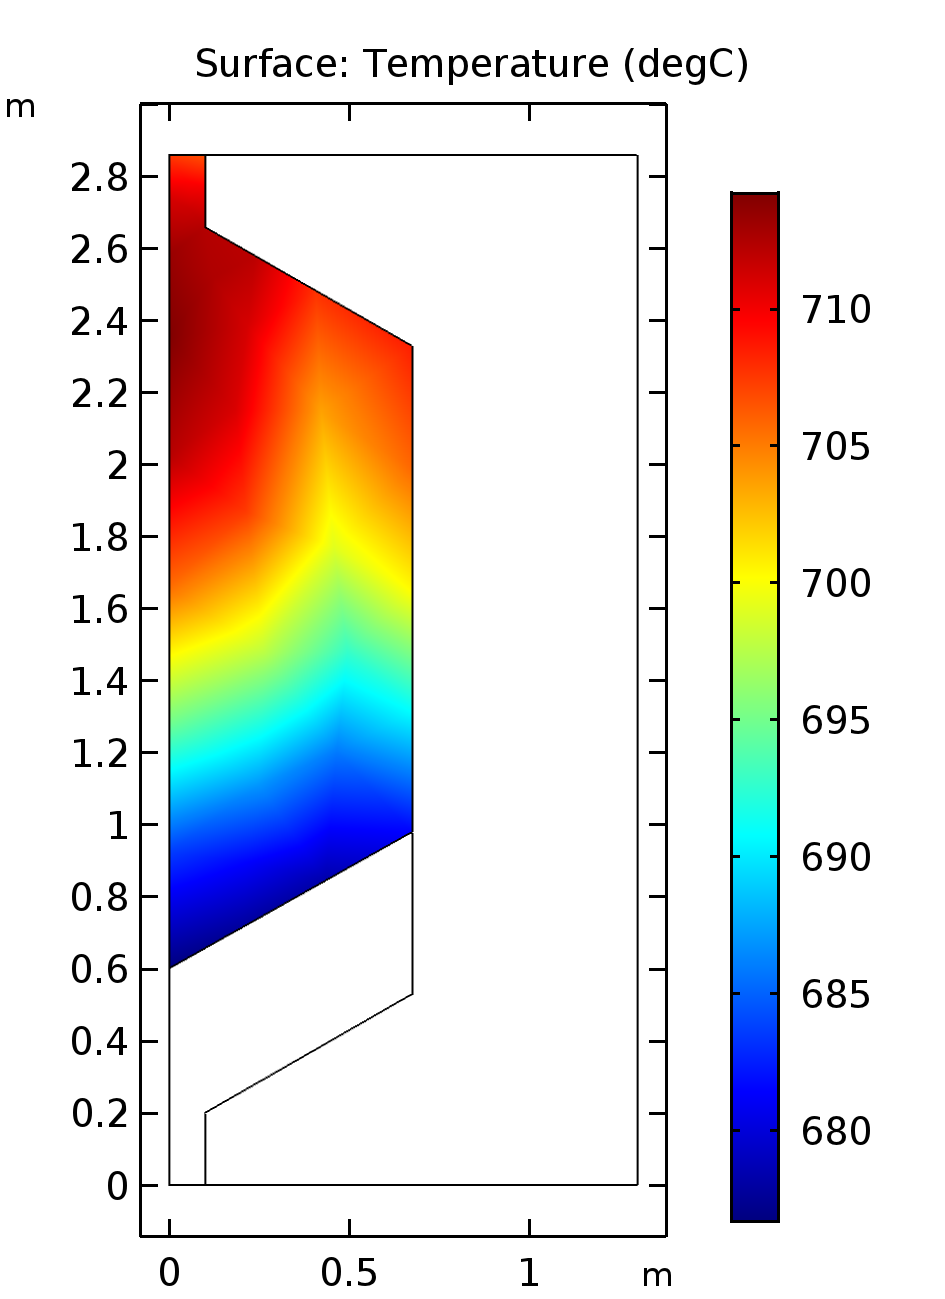
\includegraphics[width=0.9\textwidth]{./images/diffusion/tmsr/SS/non_ms/T_fuel(steady_state).png}
        \caption{Fuel}
    \end{subfigure}

  \caption{Steady state temperatures in TMSR SF-1 core, without multiscale treatment}
  \label{fig:tmsr_temp_non_ms_ss}
\end{figure}

\begin{figure}[h]
  \centering
    \begin{subfigure}[b]{0.3\textwidth}
        \centering
        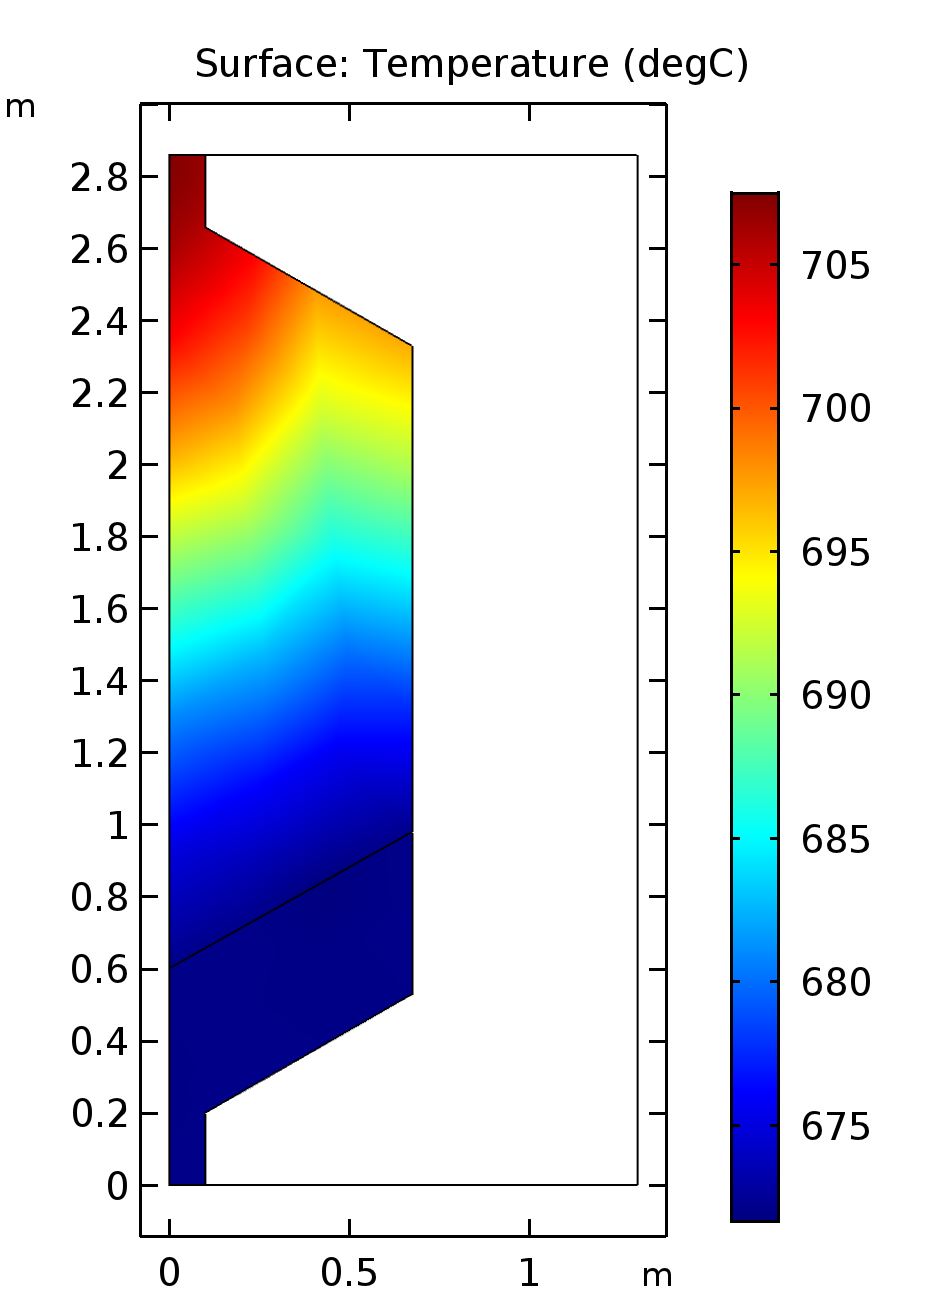
\includegraphics[width=0.9\textwidth]{./images/diffusion/tmsr/SS/ms/T_flibe(steady_state).png}
        \caption{Flibe}
    \end{subfigure}%
    ~
    \begin{subfigure}[b]{0.3\textwidth}
        \centering
        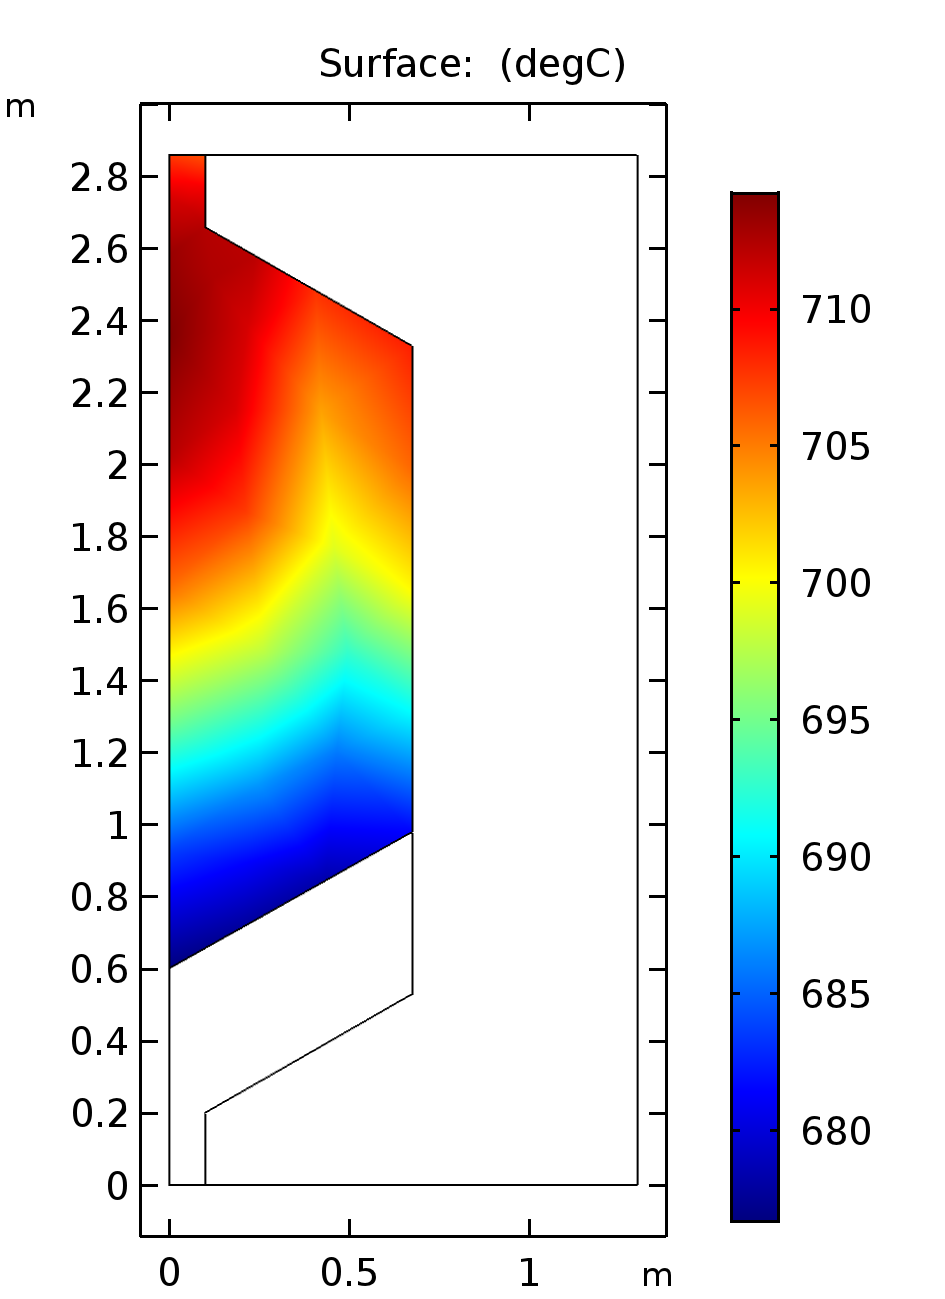
\includegraphics[width=0.9\textwidth]{./images/diffusion/tmsr/SS/ms/T_fuel(steady_state).png}
        \caption{Fuel surface}
    \end{subfigure}
    ~
    \begin{subfigure}[b]{0.3\textwidth}
        \centering
        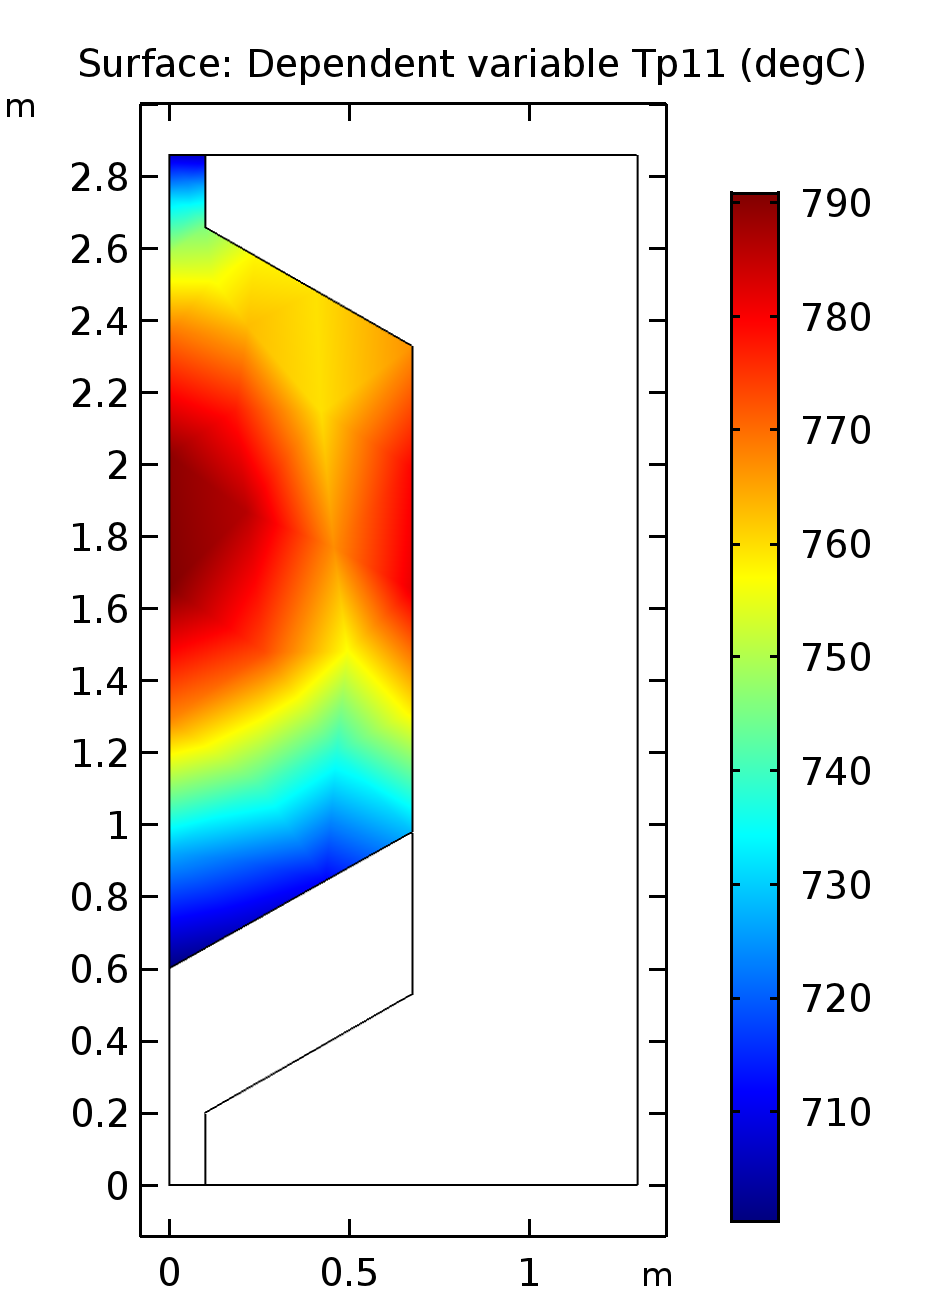
\includegraphics[width=0.9\textwidth]{./images/diffusion/tmsr/SS/ms/Tp11(steady_state).png}
        \caption{Inner TRISO fuel layer}
    \end{subfigure}

  \caption{Steady state temperatures of coolant and selected locations in fuel element in TMSR SF-1 core, with multiscale treatment}
  \label{fig:tmsr_temp_ss}
\end{figure}



The fuel temperature distribution resembles the power profile: hottest in the center and coldest at the two axial extremities, within a range between 1000K and 1120 K. 
The coolant enters the bottom of the core at 672$^{\circ}C$ and gradually heats up to 708$^{\circ}C$ as it flows through the fuel region.
Because of the large volumetric heat capacity of flibe, the coolant is a very efficient heat carrier in TMSR. Both coolant and fuel have large temperature margin below safety limit, which makes TMSR core very robust to transients.

Under the standard porous media model, a fluid temperature and a solid temperature are computed at each two dimensional points in the core. Beyond this, the multiscale treatment in the model tracks the heat transfer inside solid fuel elements and computes a set of temperatures that represents the temperature profile at various depth of the fuel elements. The resulting temperatures with or without the multiscale treatment at steady state are compared in figure \ref{fig:tmsr_temp_ss} and \ref{fig:tmsr_temp_non_ms_ss}.
At steady state, it is assumed that all the nuclear power is generated in the fuel and is transported to coolant and subsequently to the secondary loop through heat exchangers. Therefore, the coolant temperature profile are very similar with or without the multiscale treatment in fuel. 
Because of the large volumetric heat capacity of flibe, the coolant is a very efficient heat carrier in FHRs.
The coolant enters the bottom of the TMSR SF-1 core at 672$^{\circ}C$, as imposed by the inlet boundary condition, and gradually heats up to, on average, 705$^{\circ}C$ as it flows through the fuel region.

Among all the temperatures computed in the solid fuel elements, only the coldest (in the pebble shell) and the hottest (in the center layer of TRISO particles) temperature in a pebble are shown in figure \ref{fig:tmsr_temp_ss} as the upper and lower bound of the solid phase temperatures. The temperature distribution in the center of the TRISO particles resembles the power profile: hottest in the center of the core and coldest at the two axial extremities, within a range between 710 and 790 $^{\circ}C$. 
The surface temperature is, on the other hand, affected both by the nuclear power and by the coolant flowing upward across the core and shifting the peak temperature upward. The hottest fuel surface temperature is attained at the top of the core, where the coolant is the hottest. 


Overall, both the coolant and the fuel are far below their respective safety limits at steady state. The large thermal margins make the TMSR SF-1 core very robust to transient scenarios. 





\section{TMSR SF-1 transient analysis}
\label{sec:TMSR_transients}

To demonstrate the model's capability in simulating transient behaviour and to understand the implication of the multiscale treatment on safety parameters, such as power, coolant temperature and temperature in the solid fuel elements, in comparison to the conventional porous media approach, reactivity insertion and overcooling transients are simulated and the results are discussed in this section. 

In the multiscale case, the average fuel temperature is computed as a volume average of all the solid layers that contains fuel material, i.e. the temperature of graphite layers are not included in the average. This can then be averaged over the two dimensional space to obtain the core average fuel temperature. And in a similar fashion, the core maximum fuel temperature in the multiscale case is the maximum temperature of the hottest power-generating layer, which is the inner-most layer in a TRISO particle that is in the inner-most layer of a fuel pebble at the center of the core. 



\subsection{Reactivity insertion transients}


\begin{figure}
    \centering
    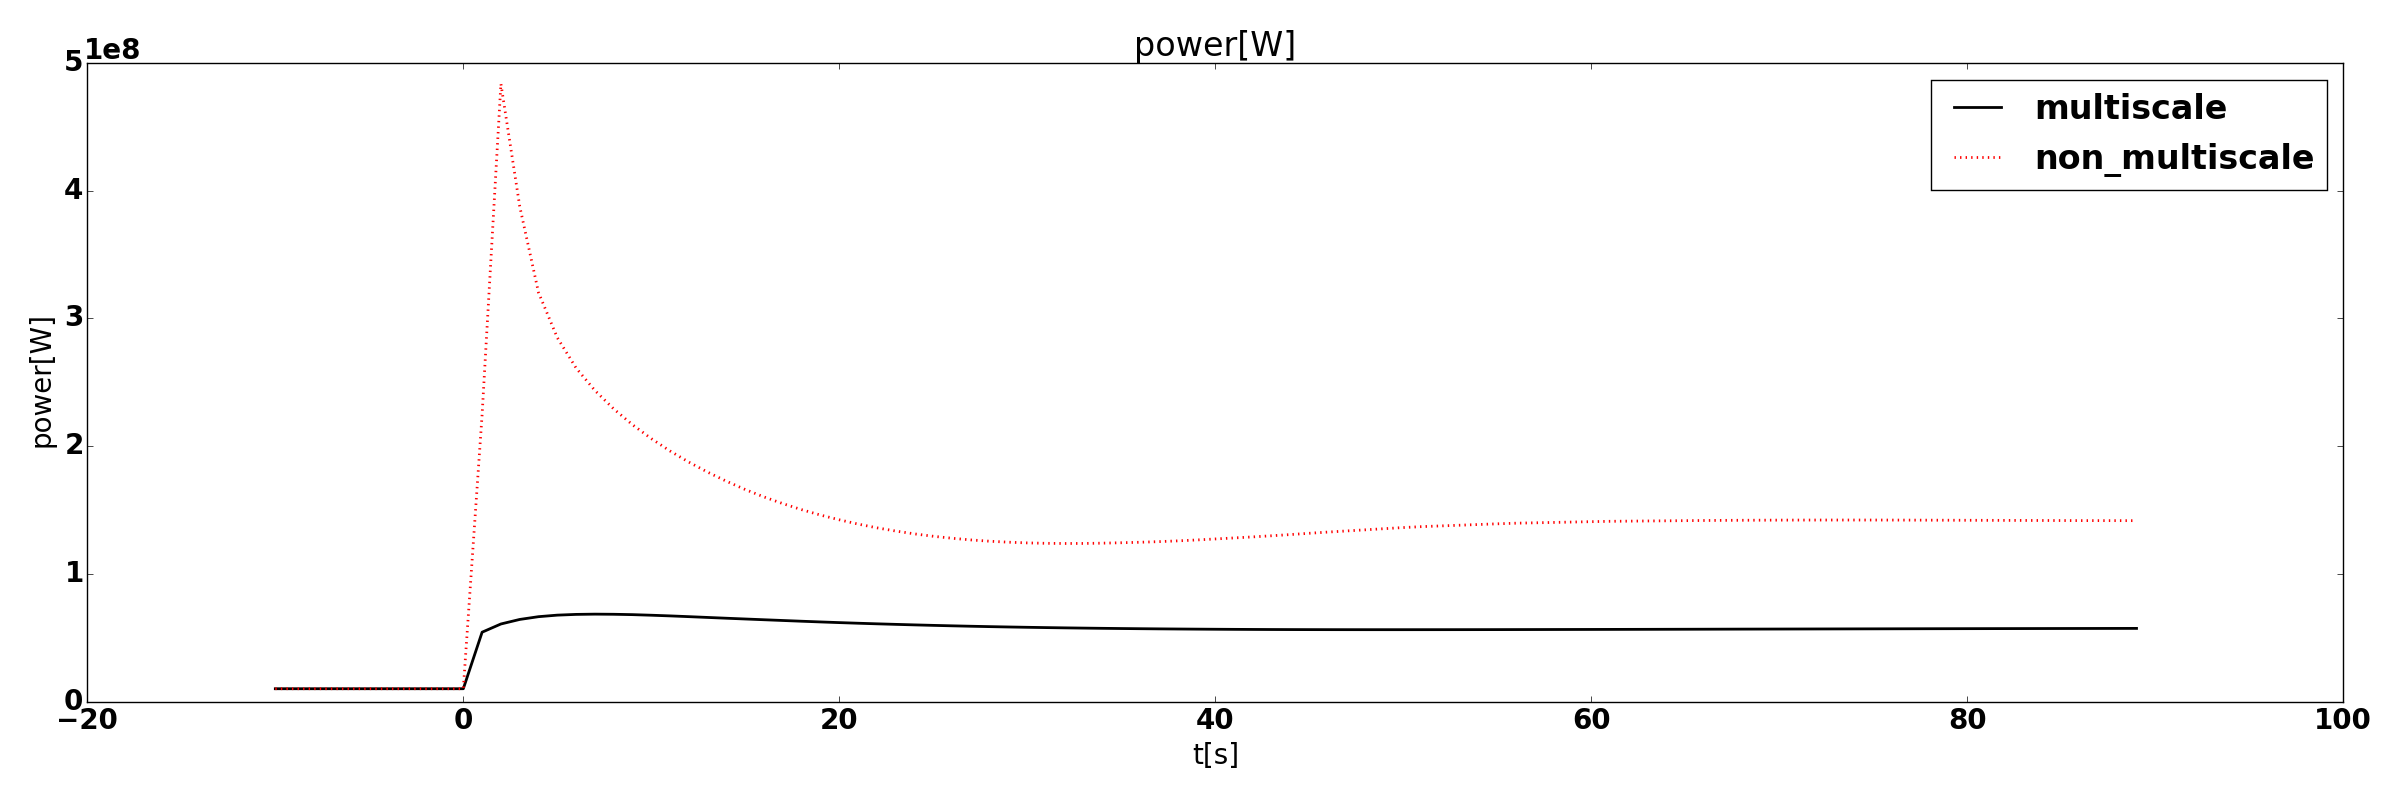
\includegraphics[width=\textwidth]{images/diffusion/tmsr/RI/compare_multiscale/power.png}
    \caption{Full core power during a 1\$ reactivity insertion transient in TMSR SF-1, with or without multiscale treatment}
    \label{fig:multi_comp_power_TMSR}
\end{figure}

\begin{figure}
    \centering
    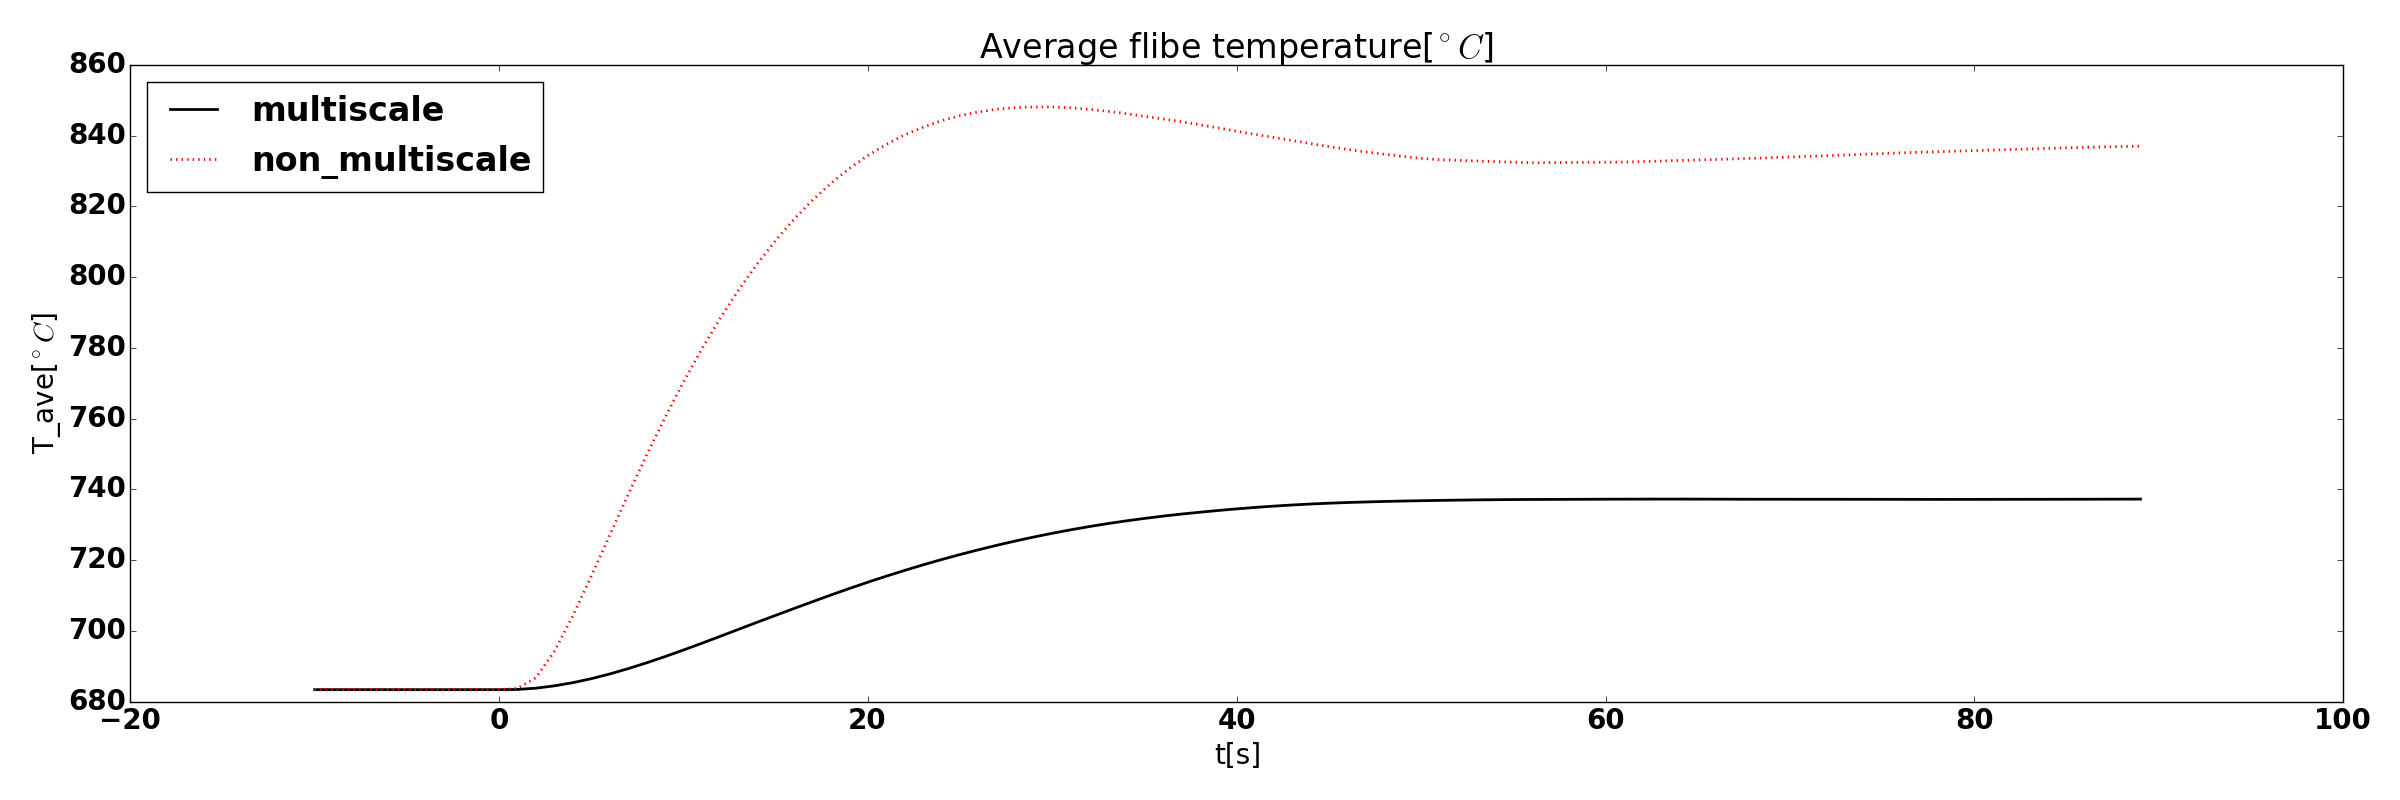
\includegraphics[width=\textwidth]{images/diffusion/tmsr/RI/compare_multiscale/T_flibe_ave.png}
    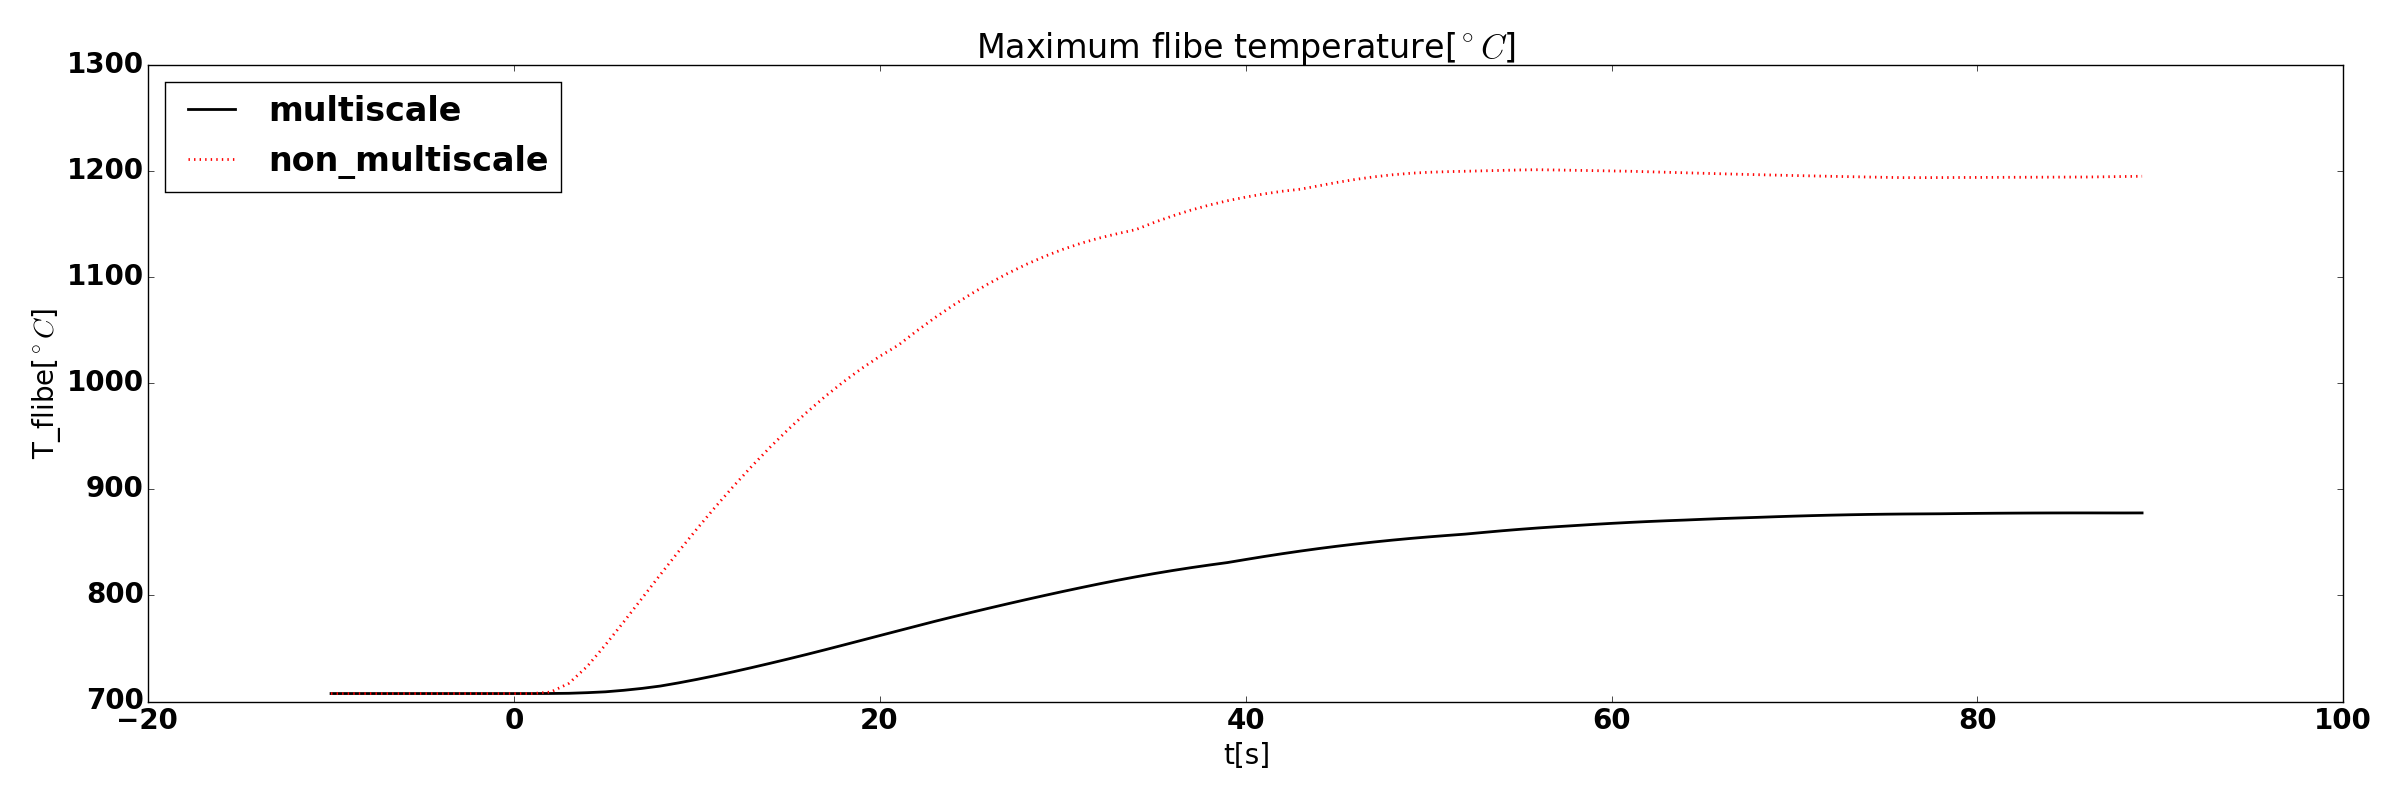
\includegraphics[width=\textwidth]{images/diffusion/tmsr/RI/compare_multiscale/T_flibe_max.png}
    \caption{Average and maximum flibe temperatures during a 1\$ reactivity insertion transient in TMSR SF-1, with or without multiscale treatment}
    \label{fig:multi_comp_flibe_TMSR}
\end{figure}

\begin{figure}
    \centering
    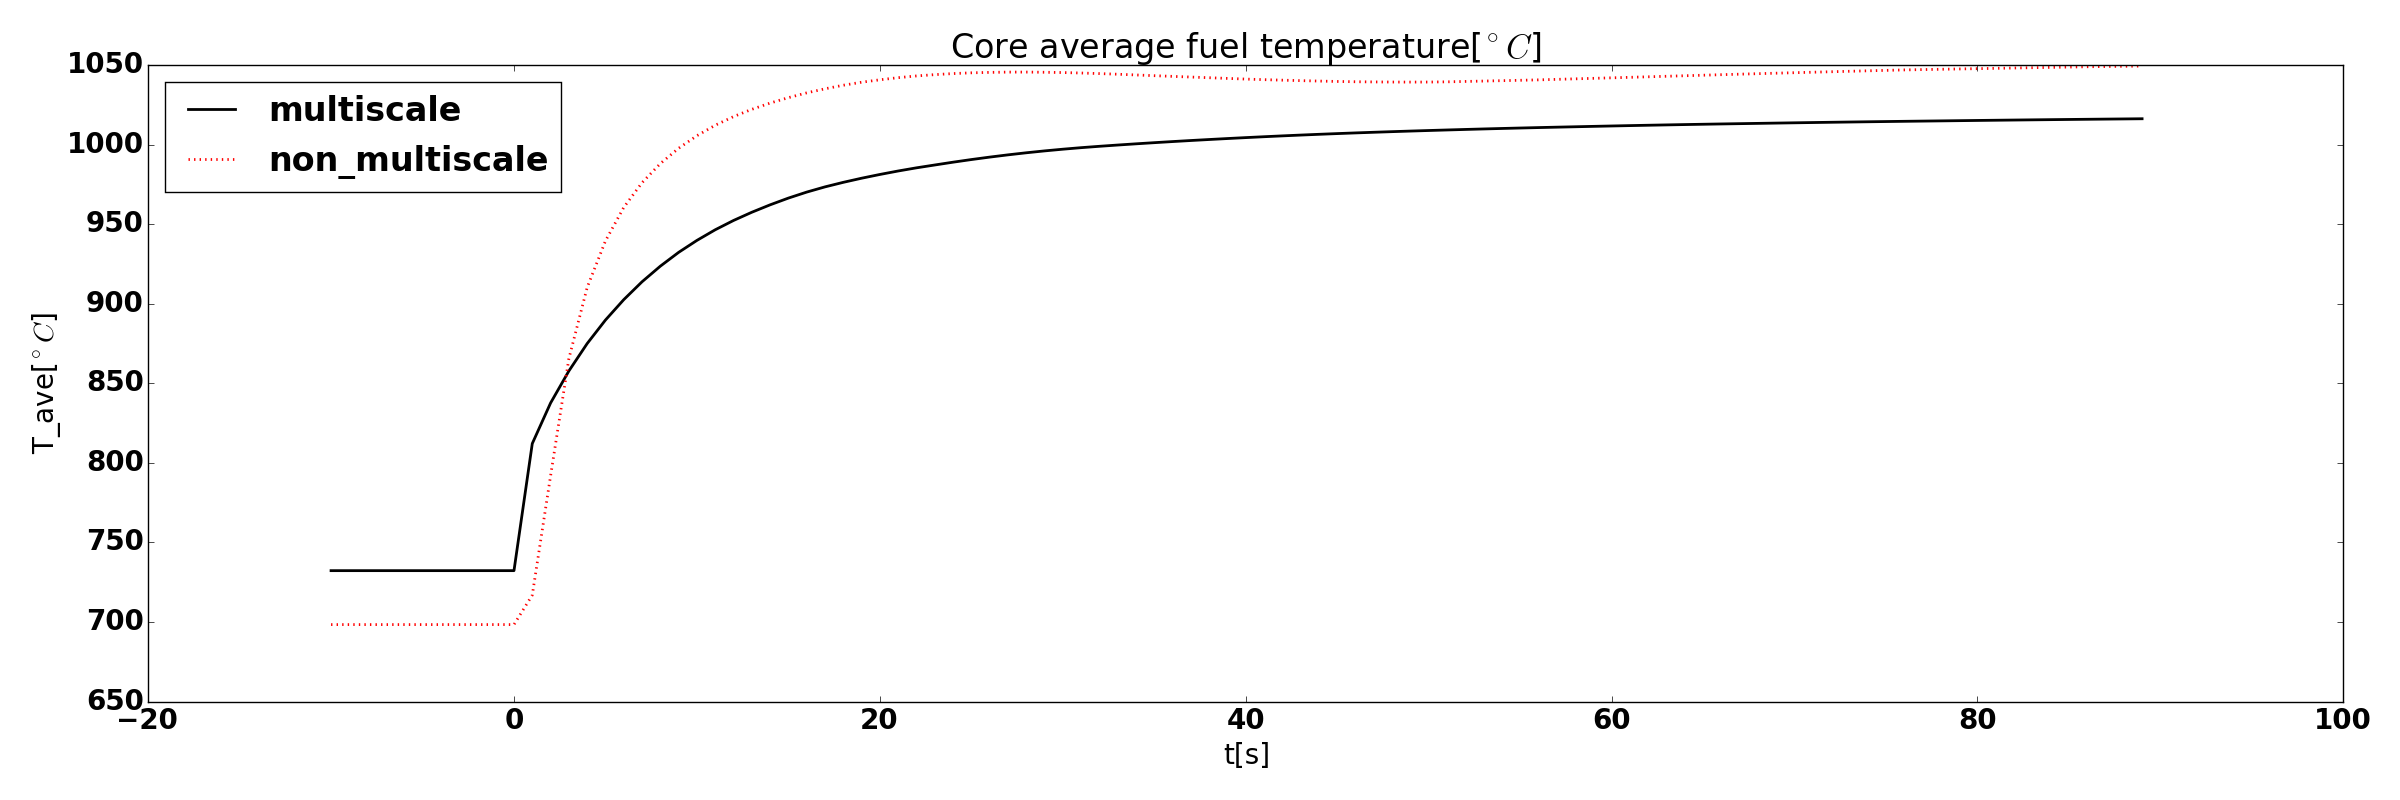
\includegraphics[width=\textwidth]{images/diffusion/tmsr/RI/compare_multiscale/T_fuel_ave.png}
    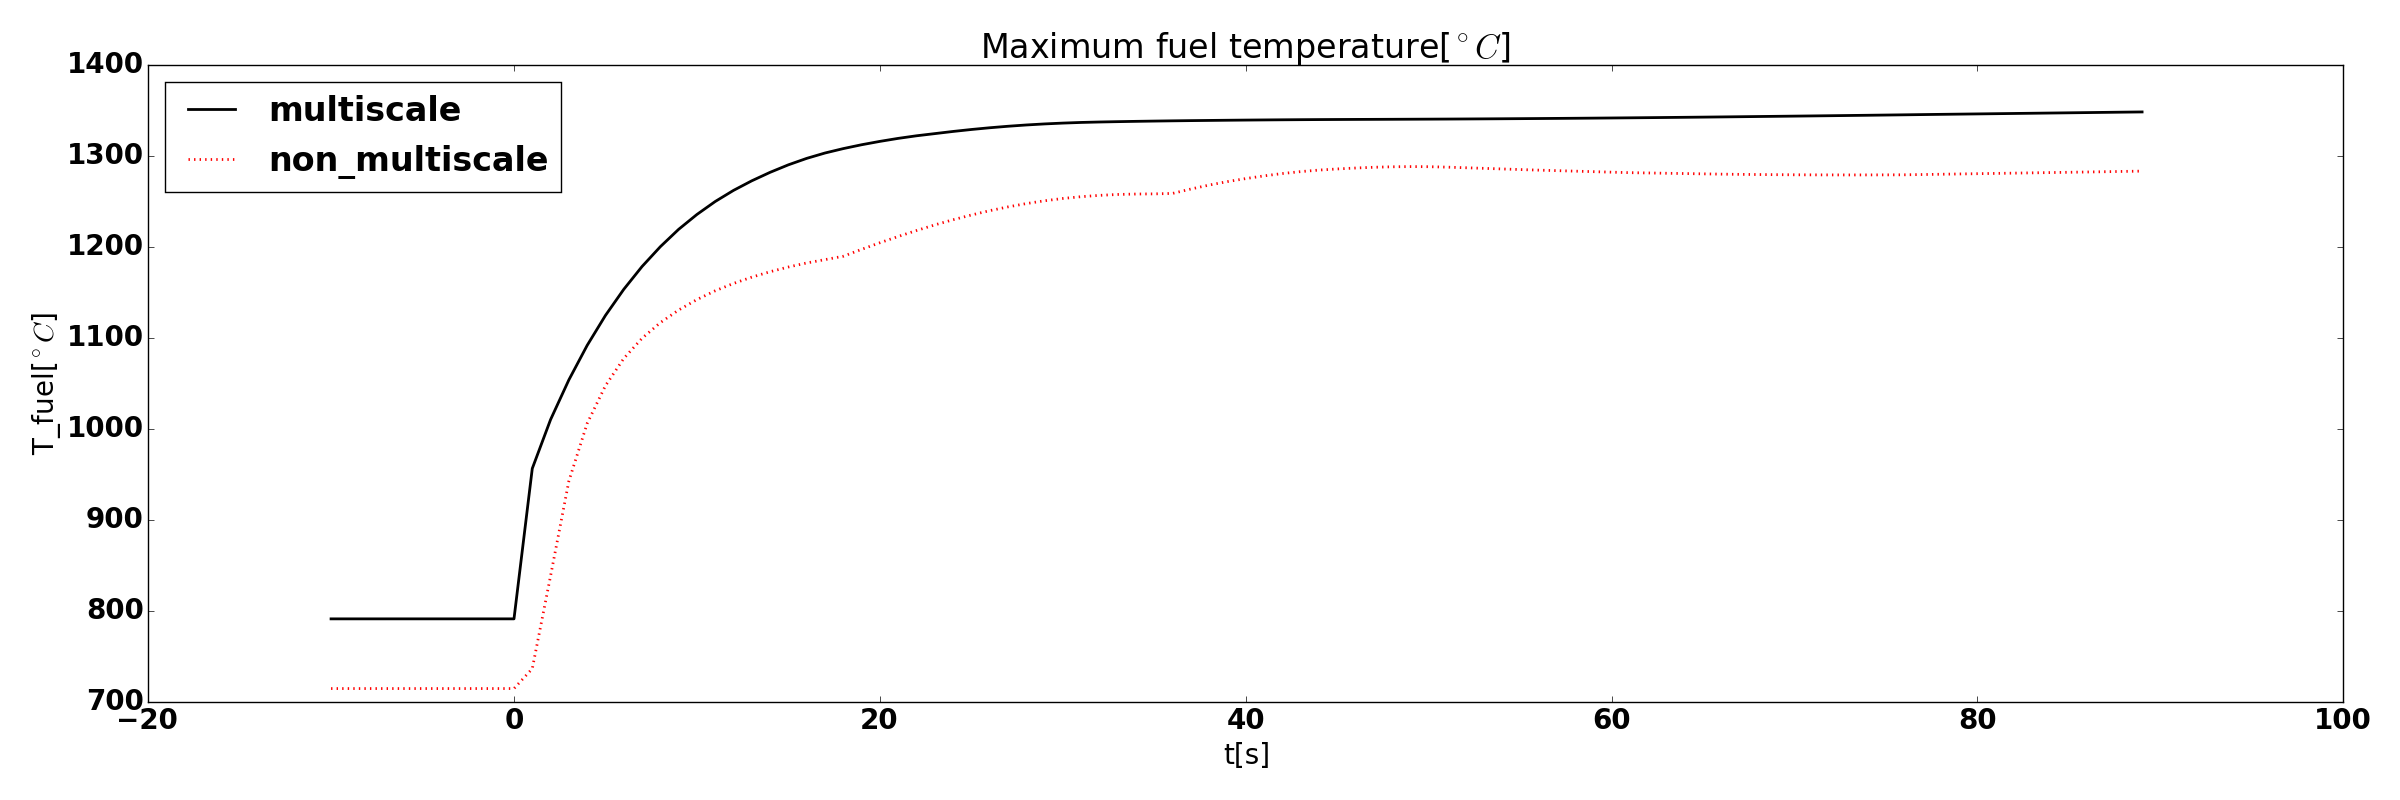
\includegraphics[width=\textwidth]{images/diffusion/tmsr/RI/compare_multiscale/T_fuel_max.png}
    \caption{Average and maximum fuel temperatures during a 1\$ reactivity insertion transient in TMSR SF-1, with or without multiscale treatment}
    \label{fig:multi_comp_fuel_TMSR}
\end{figure}

Starting from steady state under nominal conditions and with the same boundary conditions described in the previous section, 1\$ is inserted into the core at time 0. Although an insertion of 1\$ is highly unlikely due to the designed limit of the control rod, it is useful to test the model's ability to handle a large amount of reactivity insertion and to understand the core behaviour in this case as a bounding example. At the onset of the reactivity insertion transient, nuclear power rate increases due to excess of reactivity. Following the power excursion is the temperature rise in the core, first in the fuel, due to the direct deposit of the nuclear energy, and then in the coolant as the energy diffuses out of the fuel pebbles. By design, both elements provide negative temperature reactivity feedback that at the end re-stabilizes the core. 

Temperature reactivity feedback is the most important natural safety mechanism in the core during a reactivity insertion without SCRAM. In FHRs, the feedback from the Doppler broadening of the fuel resonance absorption cross-sections, i.e. the Doppler feedback, is much more prominent than the coolant void feedback. And it reacts promptly, because the Doppler feedback is directly initiated by the changes in the fuel temperature. As a result, the timescale of a reactivity insertion transient is short, shorter than the circulation time of the primary coolant, so the inlet coolant condition remains constant during the simulation.



Figure \ref{fig:multi_comp_power_TMSR} shows that the power excursion is less severe and the power stays at a lower level after the transient, when the detailed fuel temperature profile is used to compute the Doppler feedback. Also, the response is quicker in this case because the promptness of the Doppler feedback is properly captured. 


Comparison of the core average and maximum flibe temperatures between the conventional porous media model and the one with the multiscale treatment is shown in figure \ref{fig:multi_comp_flibe_TMSR}. 
The coolant flows upward through the fuel pebbles in the TMSR SF-1 core, so the hottest coolant is found at the top. In other words, the maximum coolant temperature also represents the outlet coolant temperature, one of the most important safety parameters in a FHR because this directly relates to the temperature of the metallic structures, the most vulnerable components in a FHR in terms of temperature safety margin.
The steady state flibe temperature is the same in both models, but both the average and the outlet coolant temperature rise to a higher value during the reactivity insertion transient in the non-multiscale case, the amount of heat deposited to coolant and the temperature reactivity feedback from the coolant are overestimated. 

Figure \ref{fig:multi_comp_fuel_TMSR} shows the average and maximum fuel temperature in the core during the transient, obtained with or without the mutliscale treatment. 
The peak fuel temperature in the multiscale case is higher at steady state, because the inner layers with higher temperatures are included in the average, and it remains higher during the reactivity insertion transient because of the spread in temperature inside fuel elements. On the other hand, although the average fuel temperature in the multiscale case is higher at steady state due to the higher temperatures inside the fuel elements, it is lower at the end of the transient because the reactor core stabilize at a lower power than the non multiscale case. In general, the peak fuel temperature, from which the safety margin to fuel damage is computed, is a more important safety parameter for the fuel. The conventional porous media model underestimates the peak fuel temperature during a reactivity insertion transient and could lead to an overly optimistic safety margin with respect to fuel damage during reactivity insertion transients. 

Overall, the conventional model overestimates the temperature increase in the coolant and in the average fuel temperature, whereas it underestimates the peak fuel temperature. However, when comparing the results, we need to keep in mind of the uncertainties introduced by the material properties used in both approach. In fact, pebble wise average properties are used in the non-multiscale case, whereas more detailed layer wise properties are used in the multiscale case, and large uncertainties are associated with the measurement of all these values. A large variation exists in the limited literature on TRISO fuel pebble thermal properties measurements. In addition, to simplify the computation, the outer non-power-generating layers in TRISO particles are combined into one, with an equivalent conductivity computed from the properties of the substituting materials. 
The contact resistance at the interfaces of the layers are not taken into account when computing the equivalent properties because of lack of available measurements. 

To evaluate the sensitivity of the results to the material properties, in particular thermal conductivity values of the fuel elements, figure \ref{fig:temps_TMSR} shows the core average temperatures in each TRISO and pebble layer during the 1\$ reactivity insertion transient, with either nominal material properties (table \ref{tab:triso_prop_tmsr1} and table \ref{tab:pb_prop_tmsr1}) or an uniform thermal conductivity (193 W/m.K, a typical value for nuclear graphite material) for each layer. 
In each individual TRISO particle, the center is the hottest and the temperature decreases as the heat diffuses out of the fuel material. With the nominal properties, a large temperature drop occurs at the coating due to the buffer layer. The buffer layer in a TRISO particle has a porous structure that serves as a damper to the stress caused by gaseous fission production. The porous nature of this layer makes it a thermal insulator and sets the lower bound of the conductivity. The buffer layer has the most temperature variation compare to the other layers.
In both cases, the temperatures deviate further from each other during the transient, because of the elevated power level. And the temperatures are further apart with the nominal thermal conductivity values.   

\begin{figure}
    \centering
    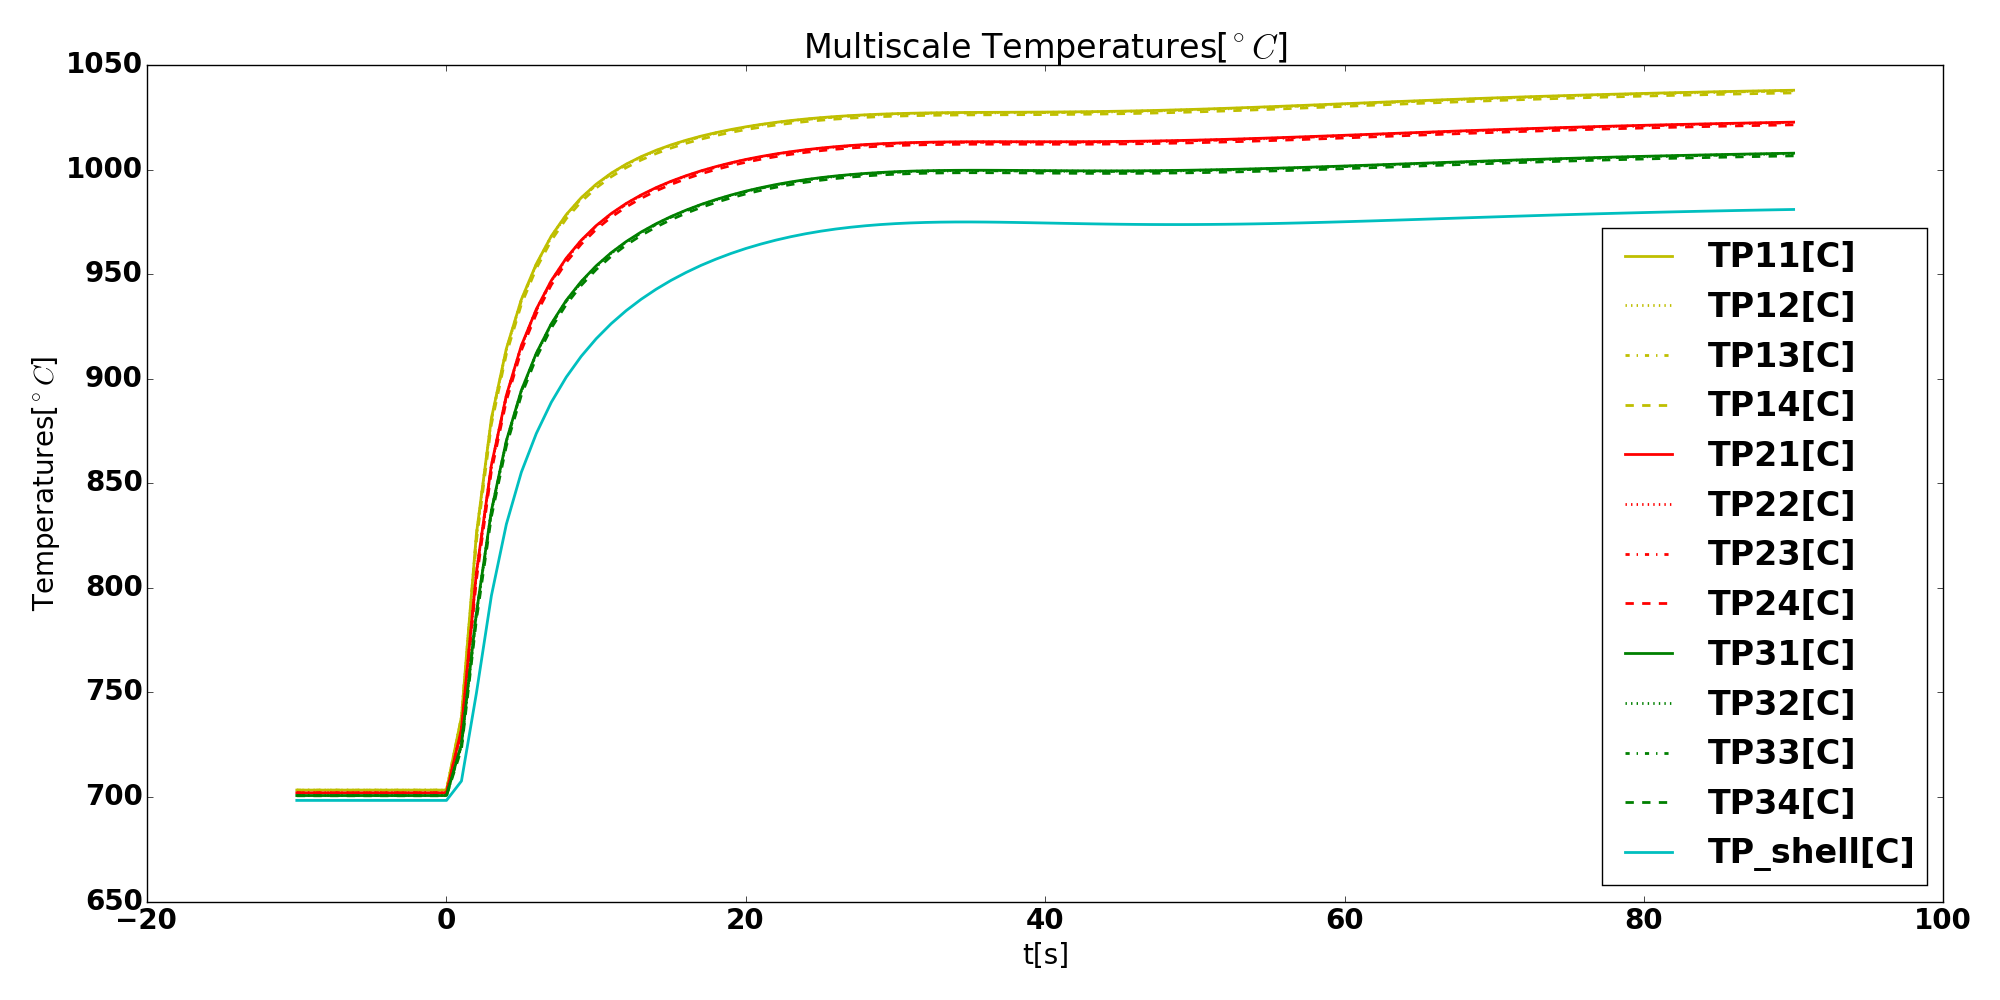
\includegraphics[width=\textwidth]{images/diffusion/tmsr/RI/compare_multiscale/temps_large_k.png}
    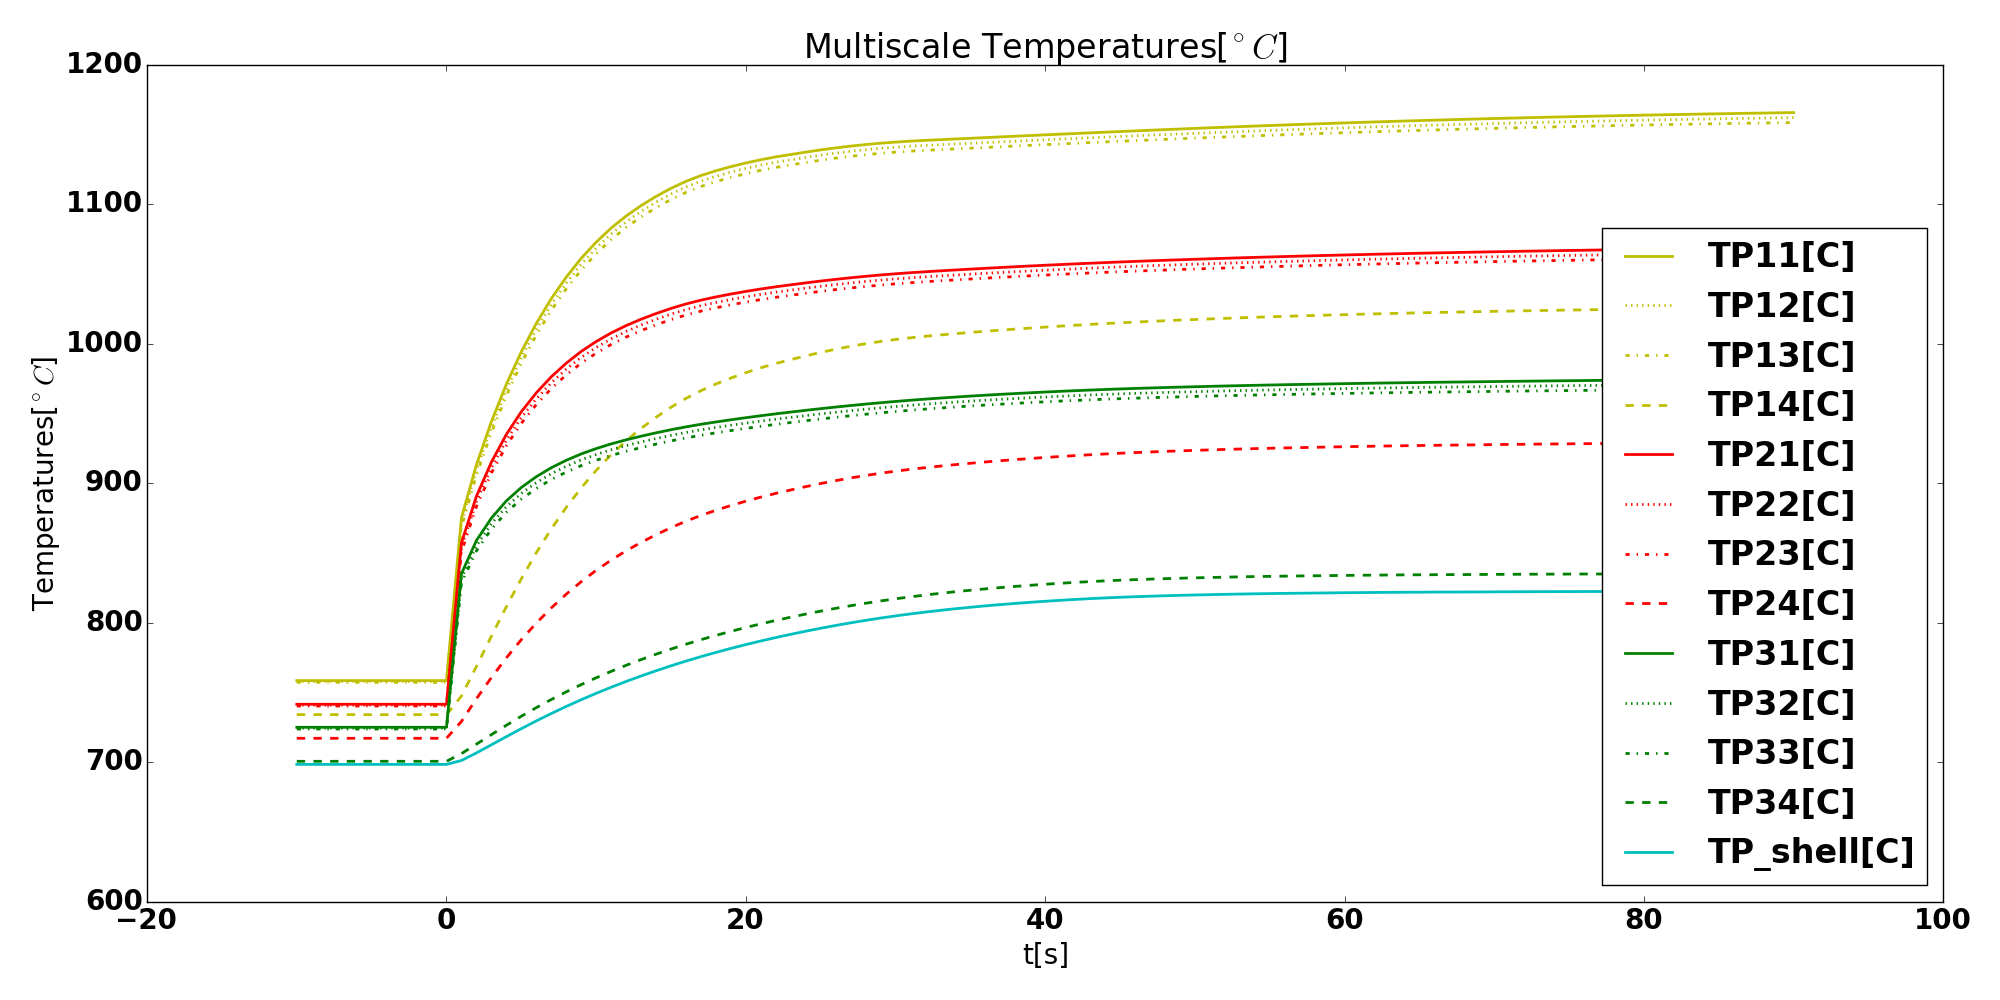
\includegraphics[width=\textwidth]{images/diffusion/tmsr/RI/compare_multiscale/temps_nominal_k.png}
    \caption{Core average temperature inside fuel elements during 1\$ reactivity insertion transient for TMSR SF-1, with a large thermal conductivity posed to all material(top) or with nominal material properties for each layer(bottom). Notation for temperatures: $TP_{ij}$ represents the jth TRISO layer in the ith pebble layer. (A fuel core in a pebble is divided into three layers and within each layer, a TRISO particle is divided into four layers - three fuel layers and one coating layer.). And $TP_{shelll}$ is the temperature in the graphite shell of the pebble.} 
    \label{fig:temps_TMSR}
\end{figure}

 
\newpage
As discussed before, the multiscale treatment is important in capturing the correct feedback behaviour, so the results shown hereafter are with the treatment.  
Figure \ref{fig:RI_pcm} shows the power and temperature evolution during a 1\$ or 0.5\$ reactivity insertion. 
 During the 1\$ prompt insertion transient, the core maximum fuel temperature is 1500$^{\circ}C$, below the safety limit(1600$^{\circ}C$). 
Coolant temperature is raised by only 100$^{\circ}C$ at the peak. 


\begin{figure}[h]
    \centering
        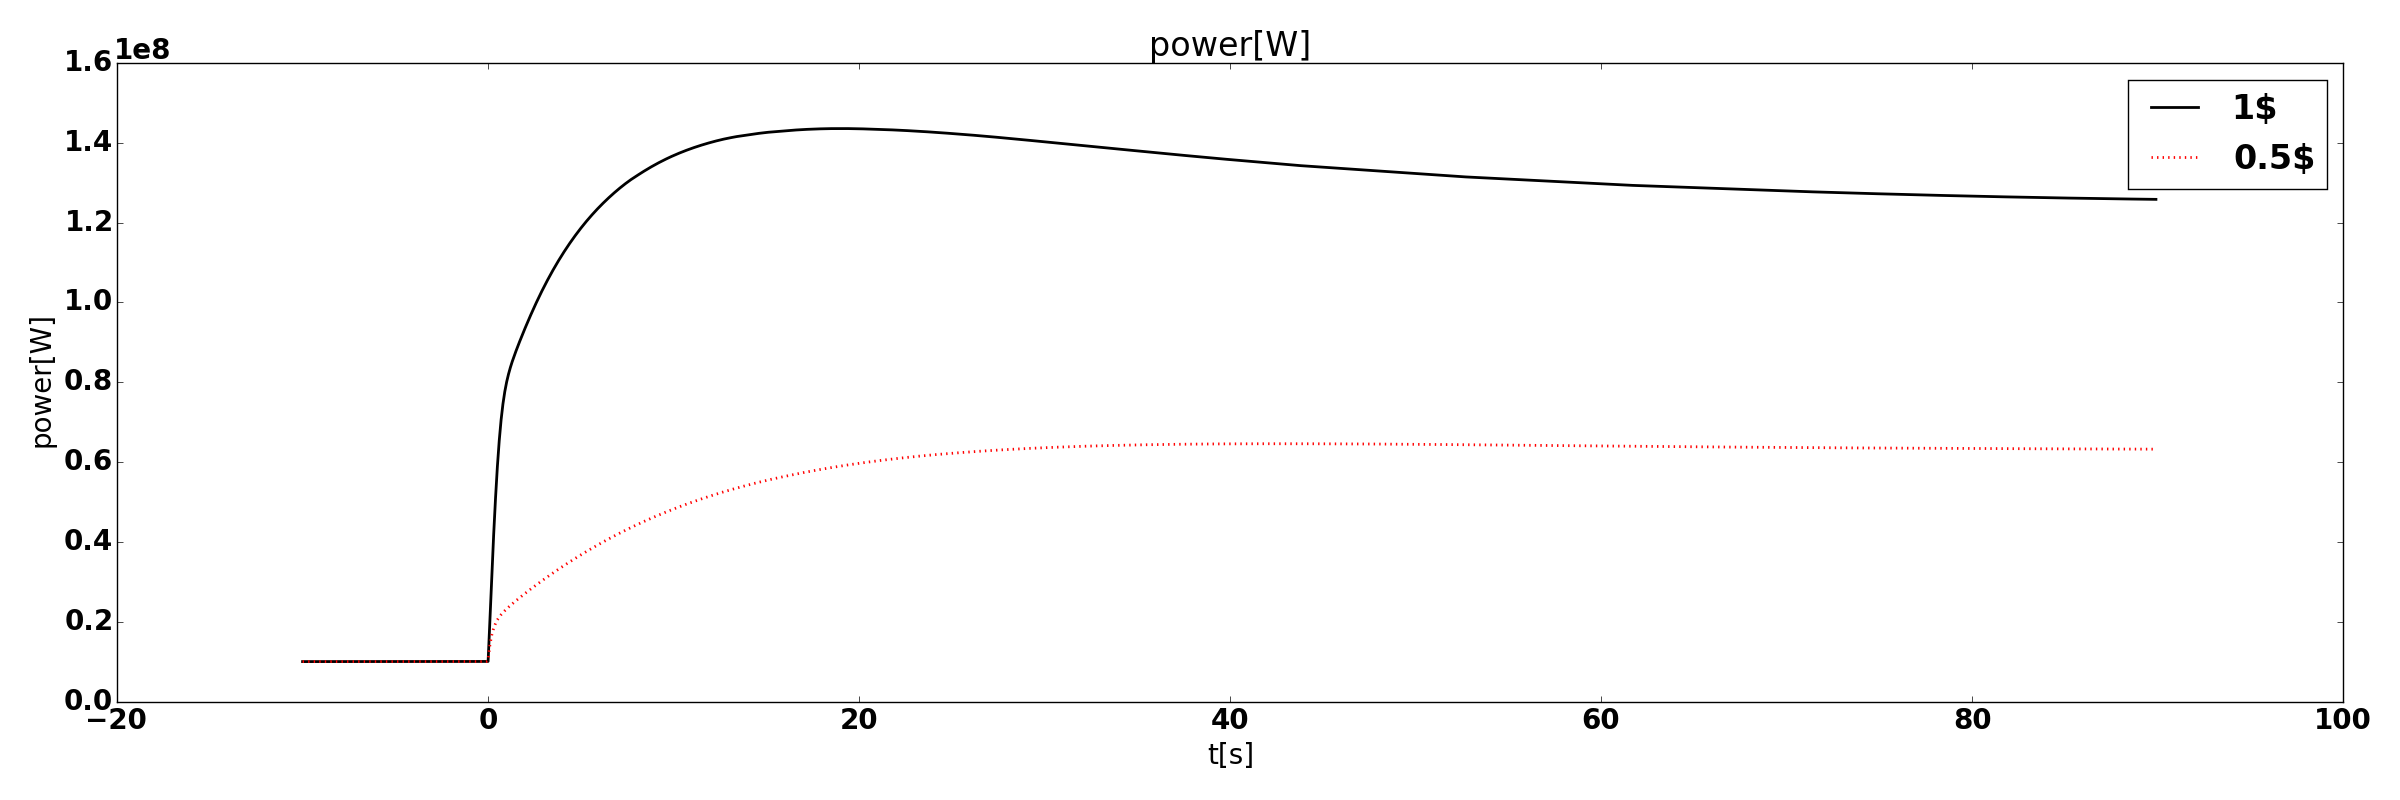
\includegraphics[width=1\linewidth]{./images/diffusion/tmsr/RI/diff_pcm/power.png}
        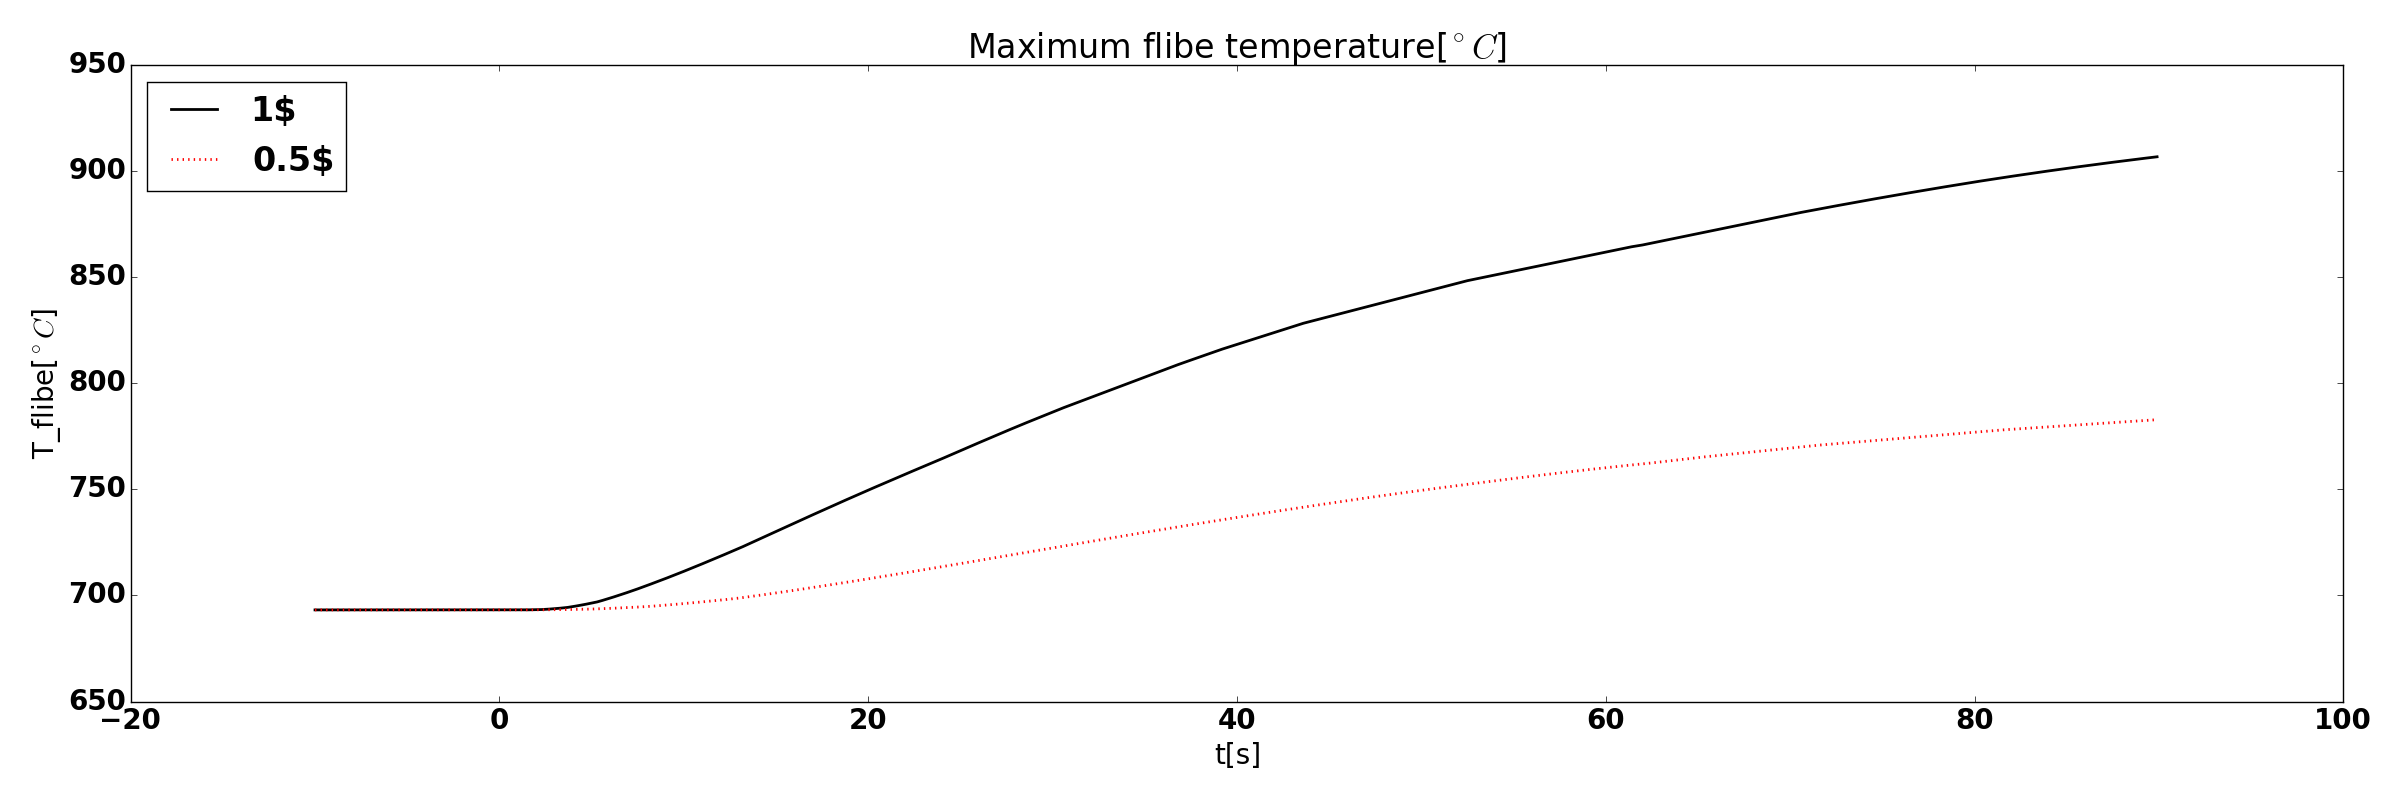
\includegraphics[width=1\textwidth]{./images/diffusion/tmsr/RI/diff_pcm/T_flibe_max.png}
        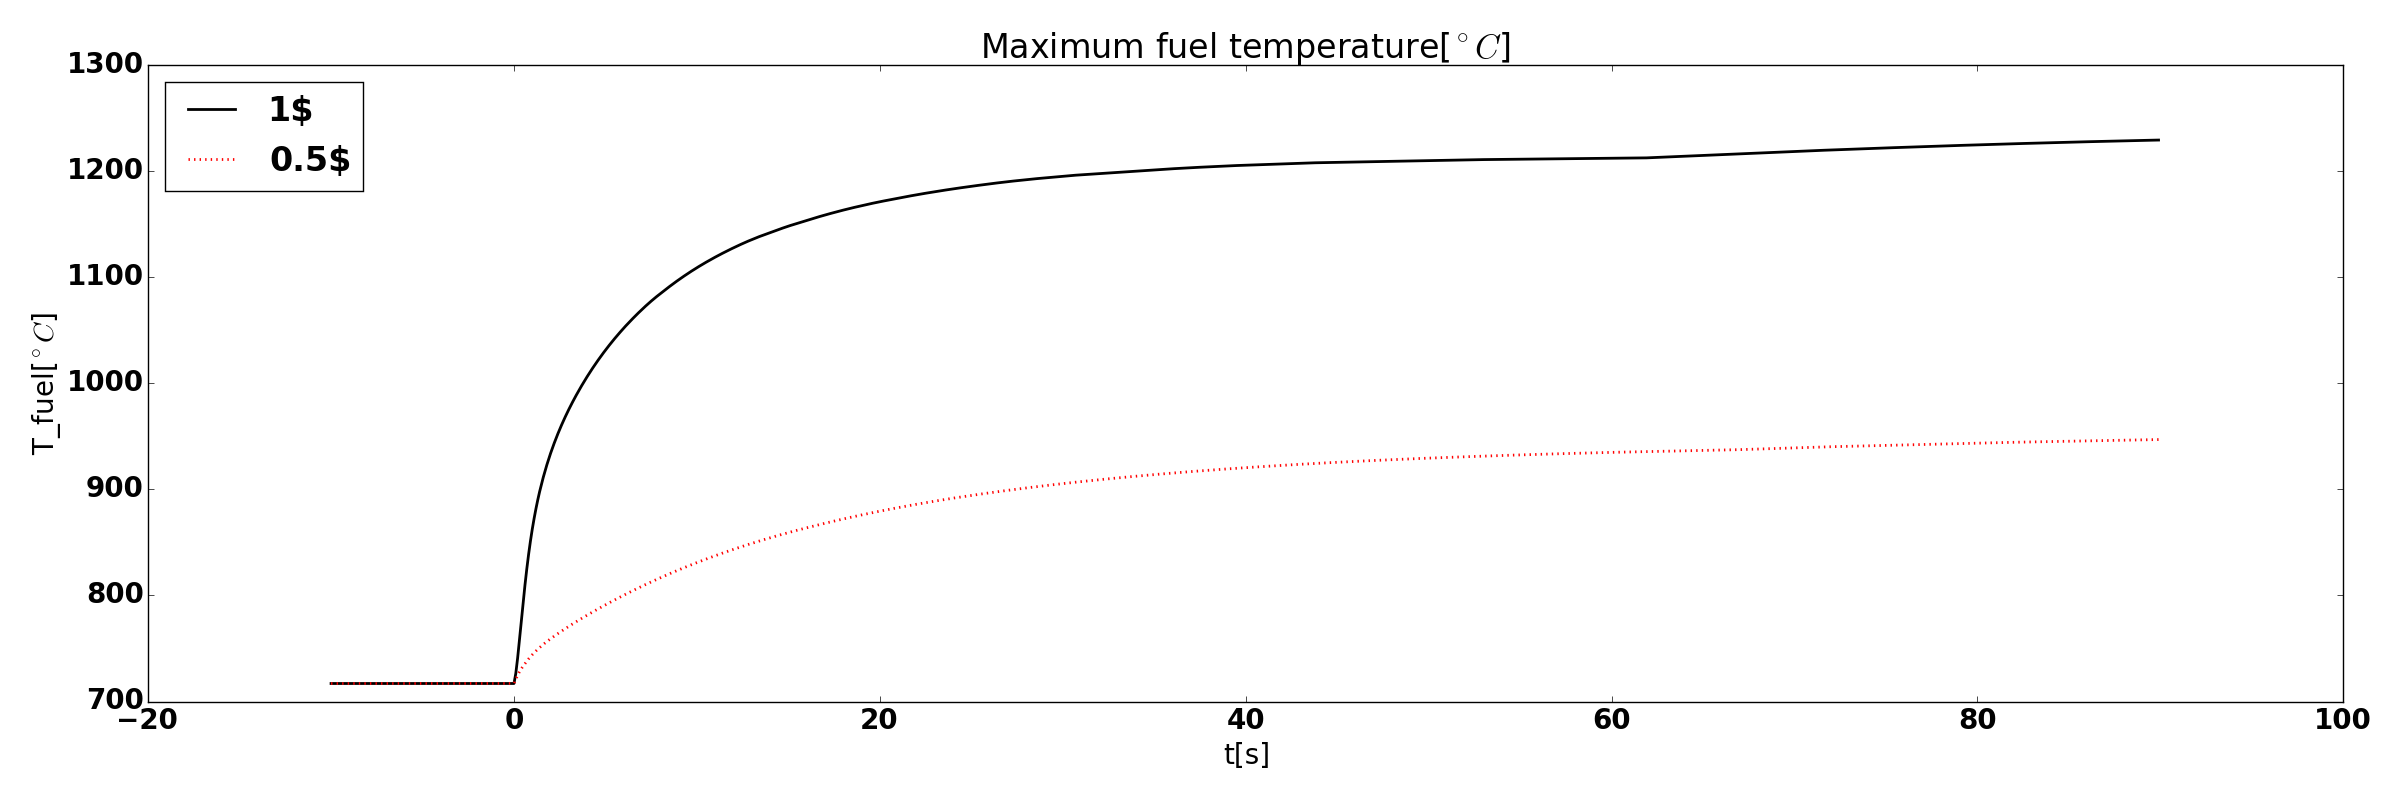
\includegraphics[width=1\textwidth]{./images/diffusion/tmsr/RI/diff_pcm/T_fuel_max.png}
    \caption{RI transients results}
    \label{fig:RI_pcm}
\end{figure}


Figure \ref{fig:RI_time} shows the effect of the timescale of the reactivity insertion on the safety parameters. Without SCRAM, the reactor reaches the same end state due to reactivity feedback mechanisms. However, safety measures can take in place to mitigate the consequence if the transient is slow. 

\begin{figure}[h]
    \centering
        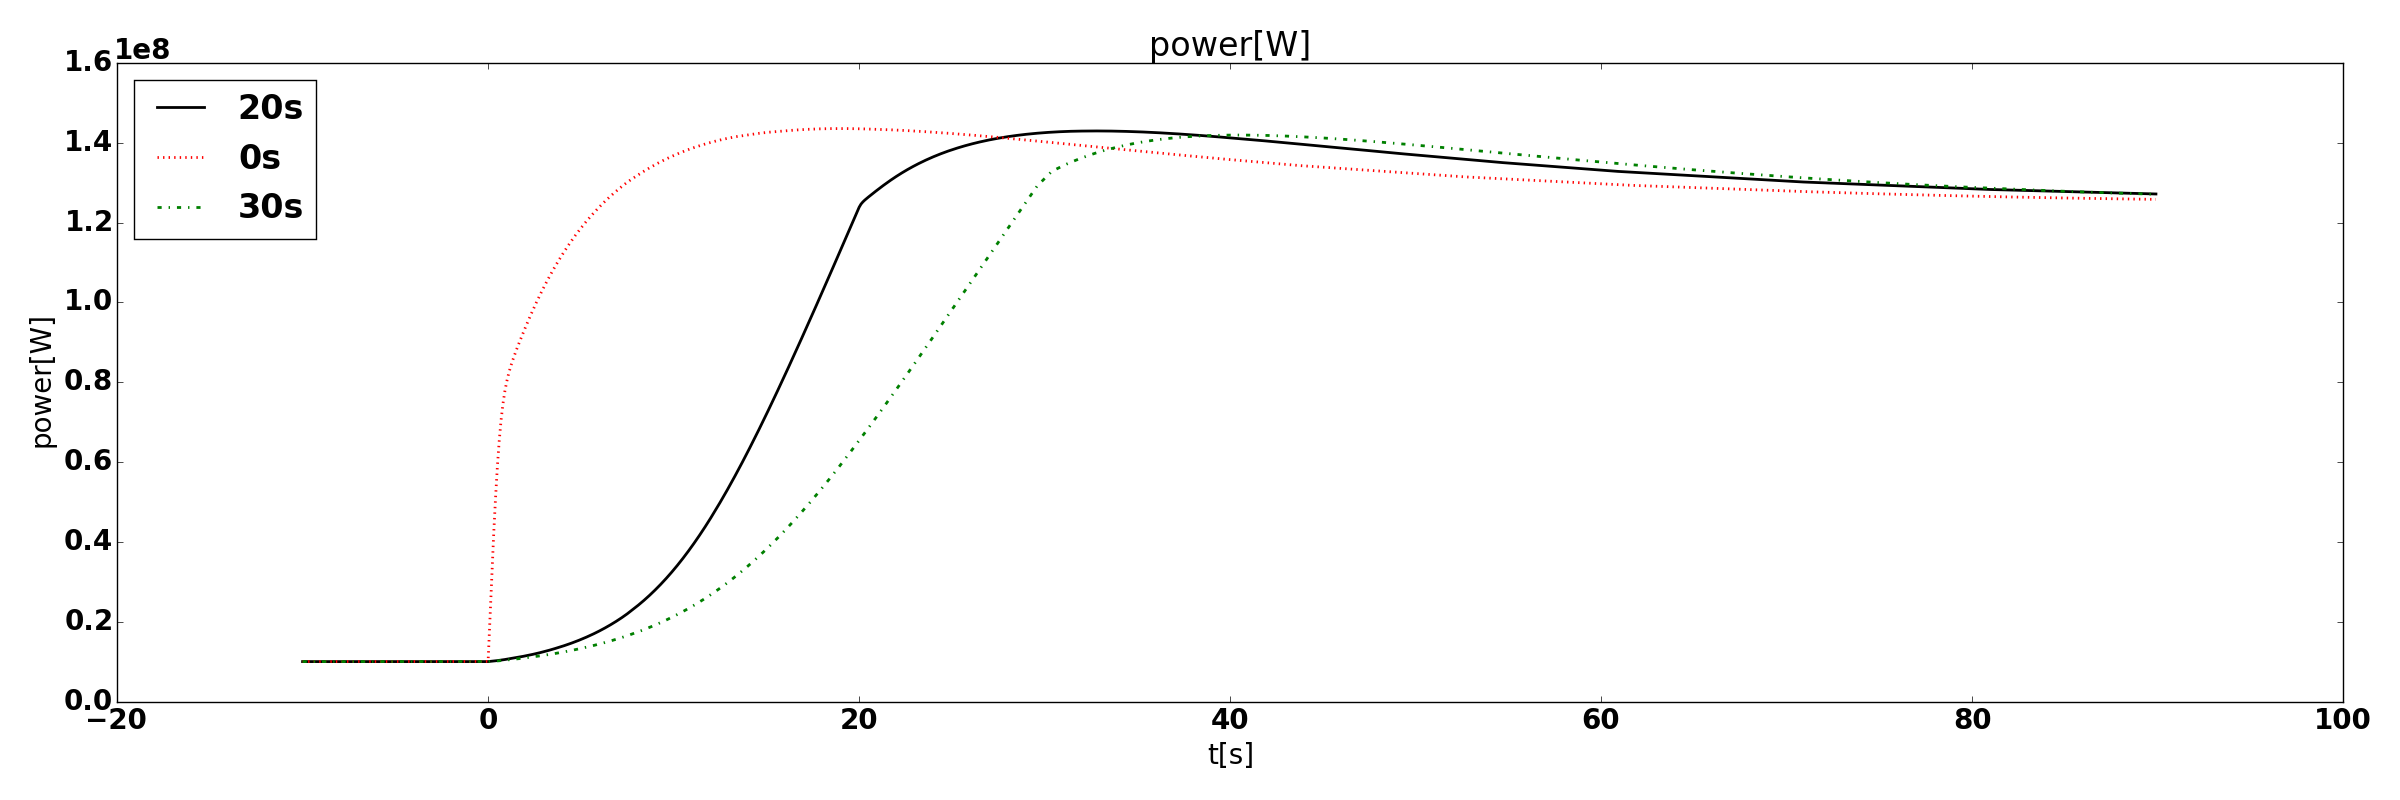
\includegraphics[width=\textwidth]{./images/diffusion/tmsr/RI/diff_time/power.png}
        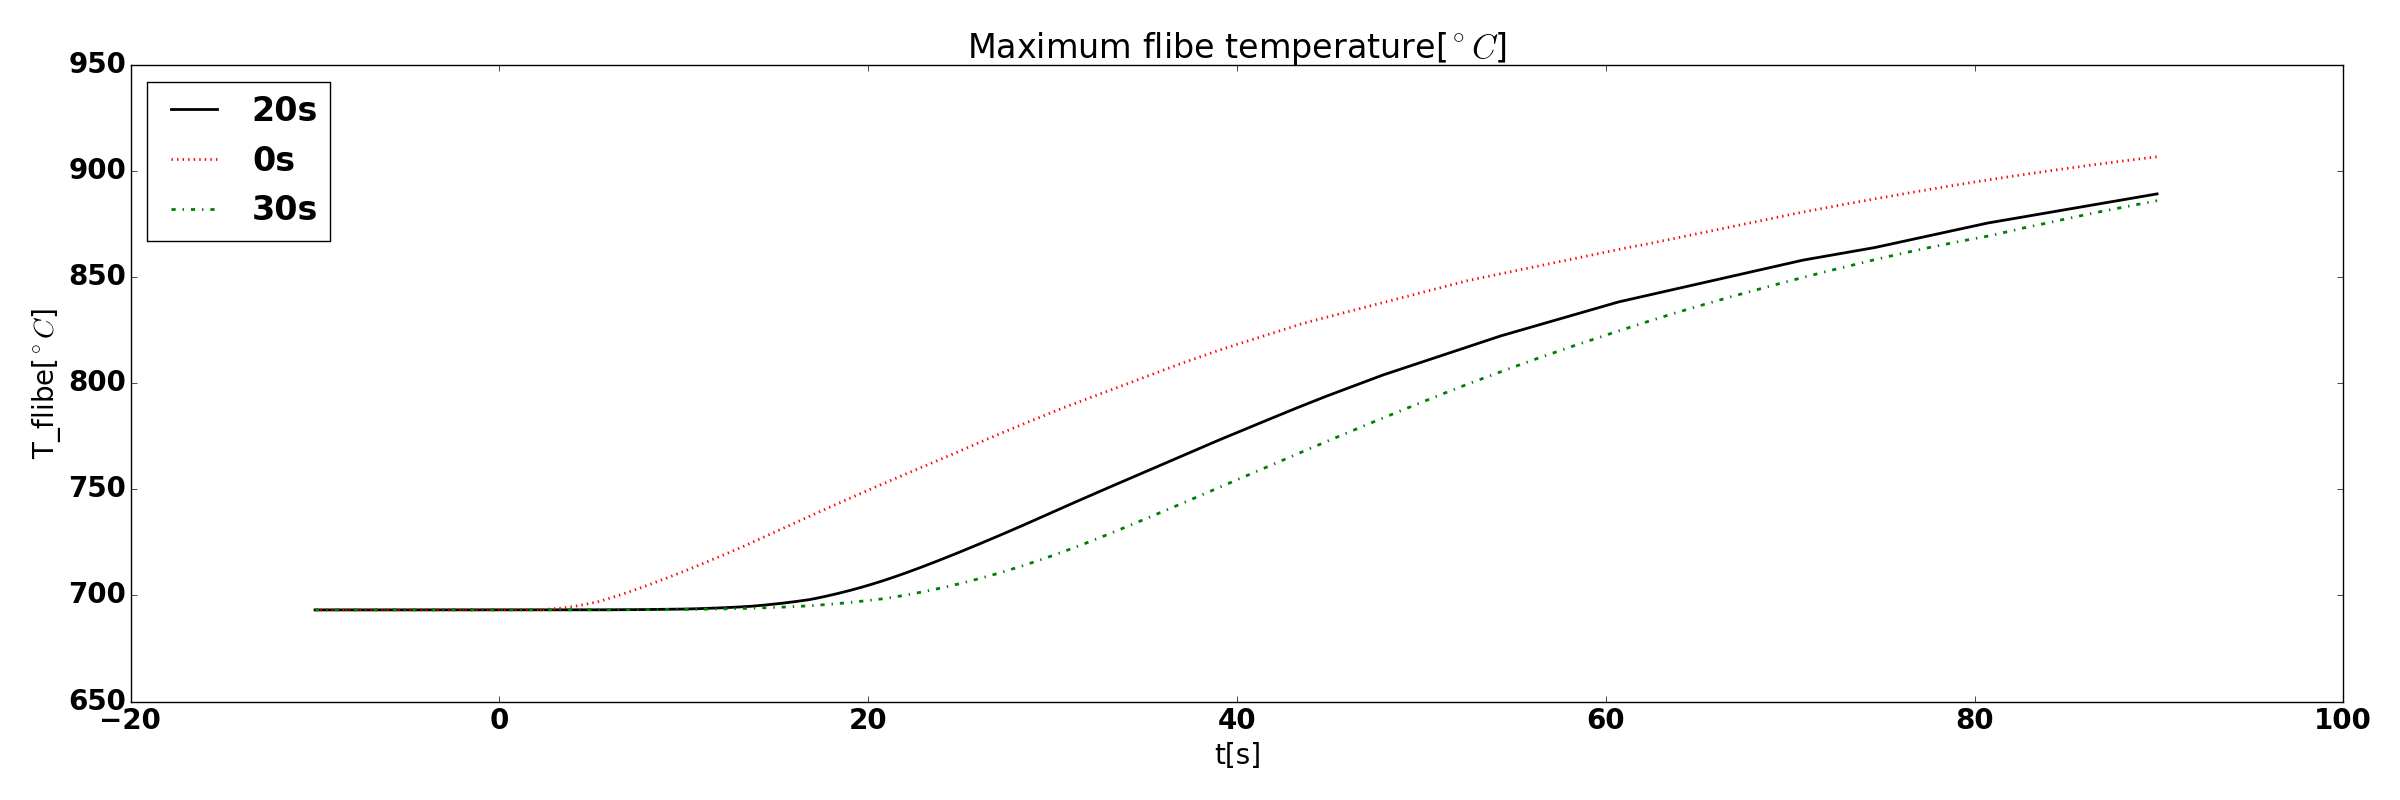
\includegraphics[width=\textwidth]{./images/diffusion/tmsr/RI/diff_time/T_flibe_max.png}
        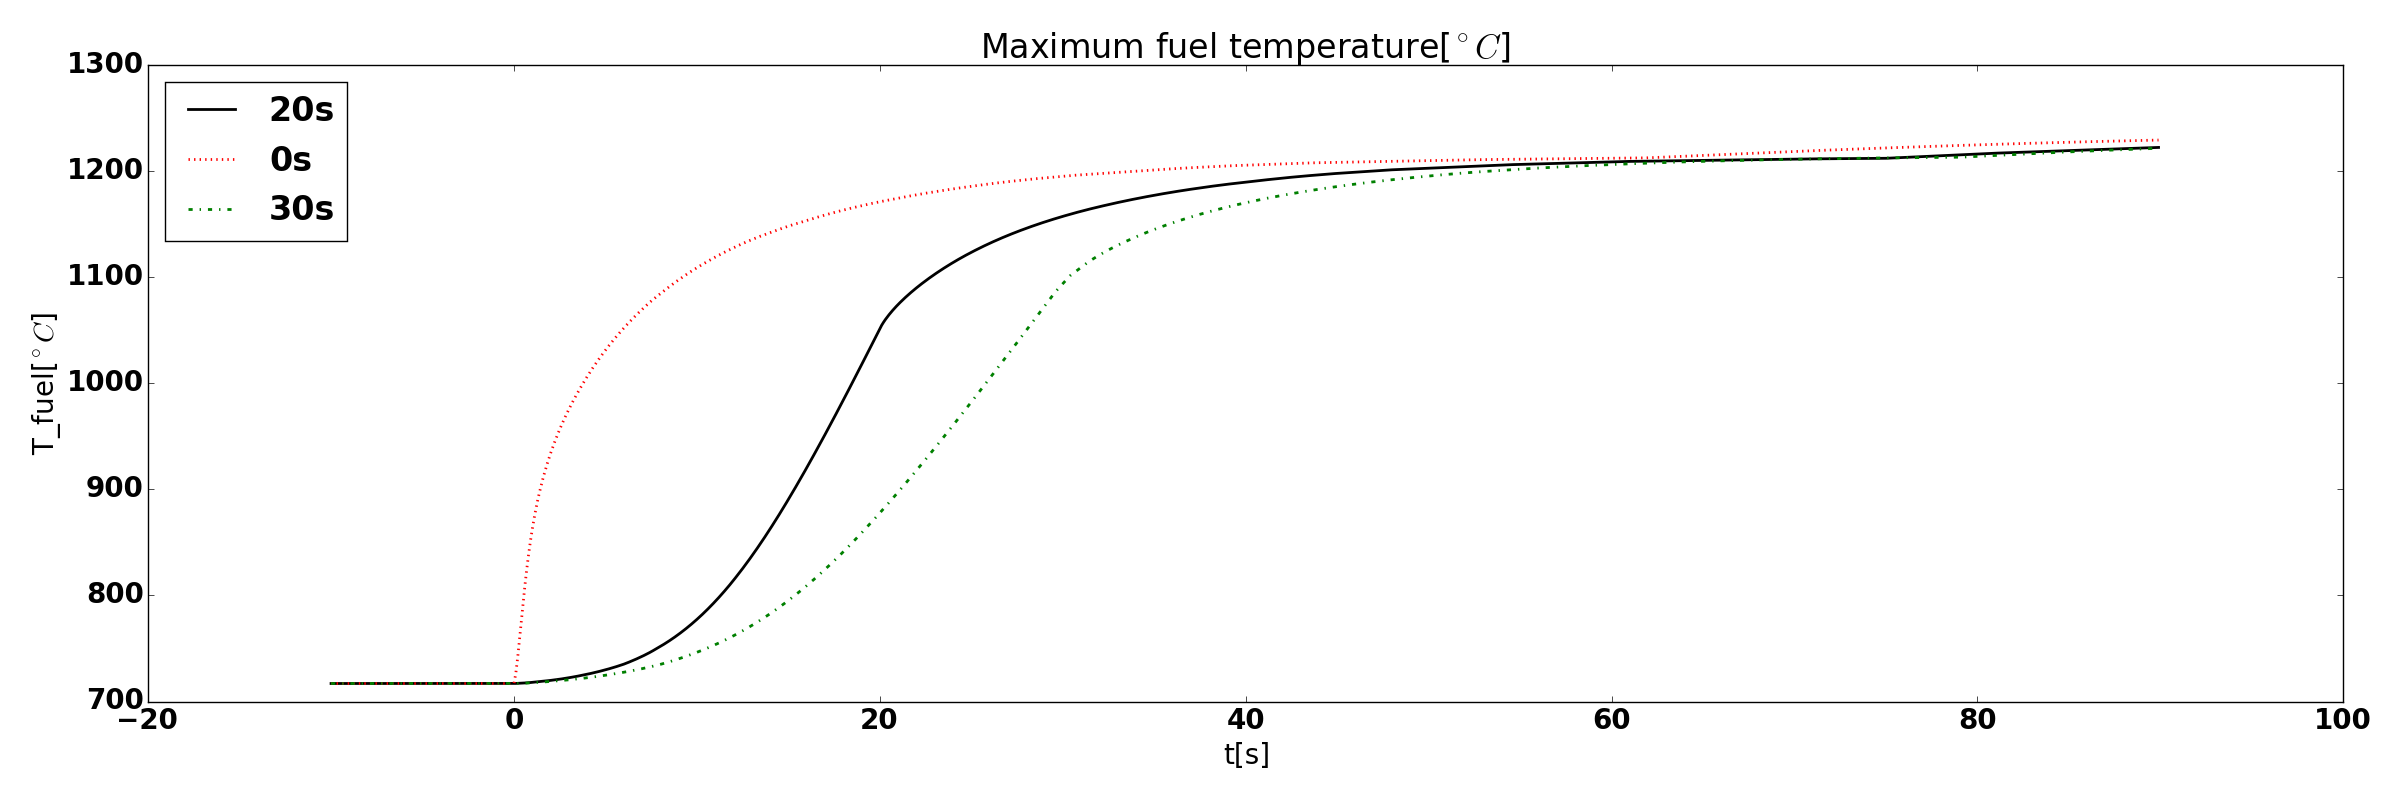
\includegraphics[width=\textwidth]{./images/diffusion/tmsr/RI/diff_time/T_fuel_max.png}
    \caption{RI transients results}
    \label{fig:RI_time}
\end{figure}




\newpage
\subsection{Overcooling transients}

\begin{figure}[h]
    \centering
        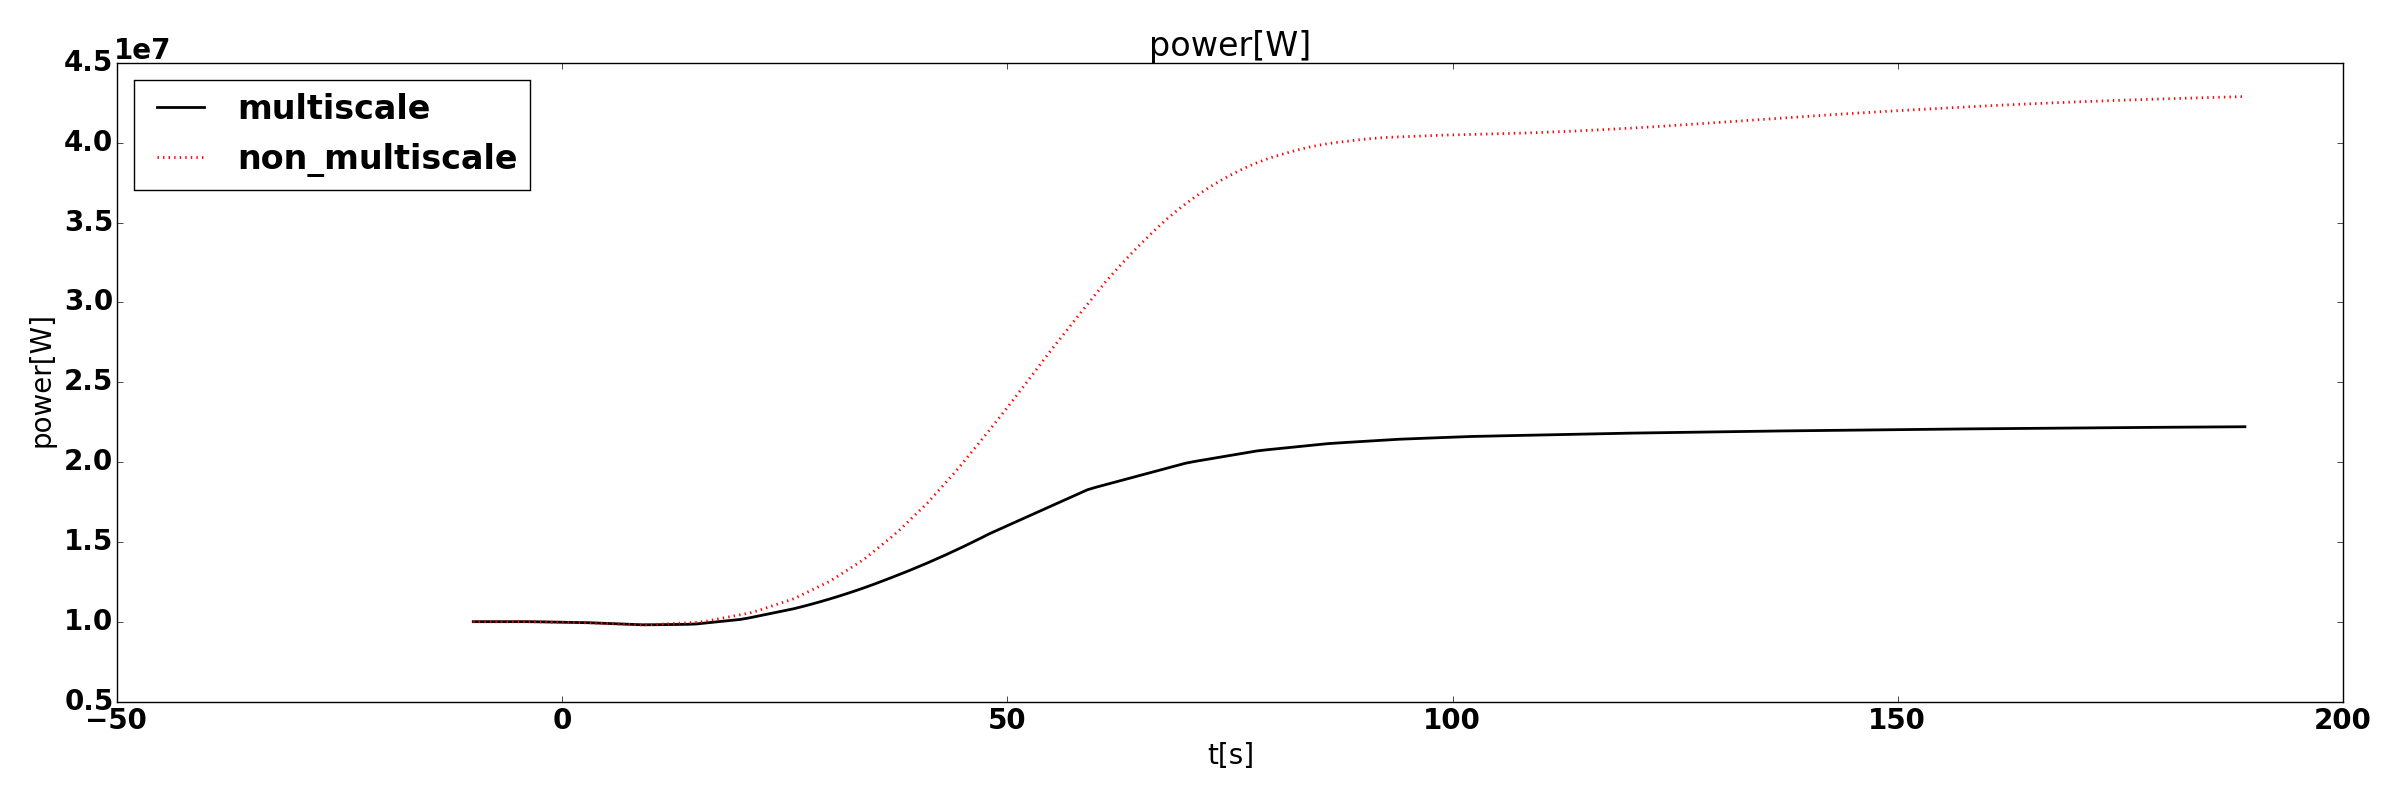
\includegraphics[width=1\linewidth]{./images/diffusion/tmsr/OC/compare_multiscale/power.png}
        \caption{Full core power during overcooling transient}
        \label{fig:OC_power}
\end{figure}


\begin{figure}[h]
    \centering
        
        \centering
        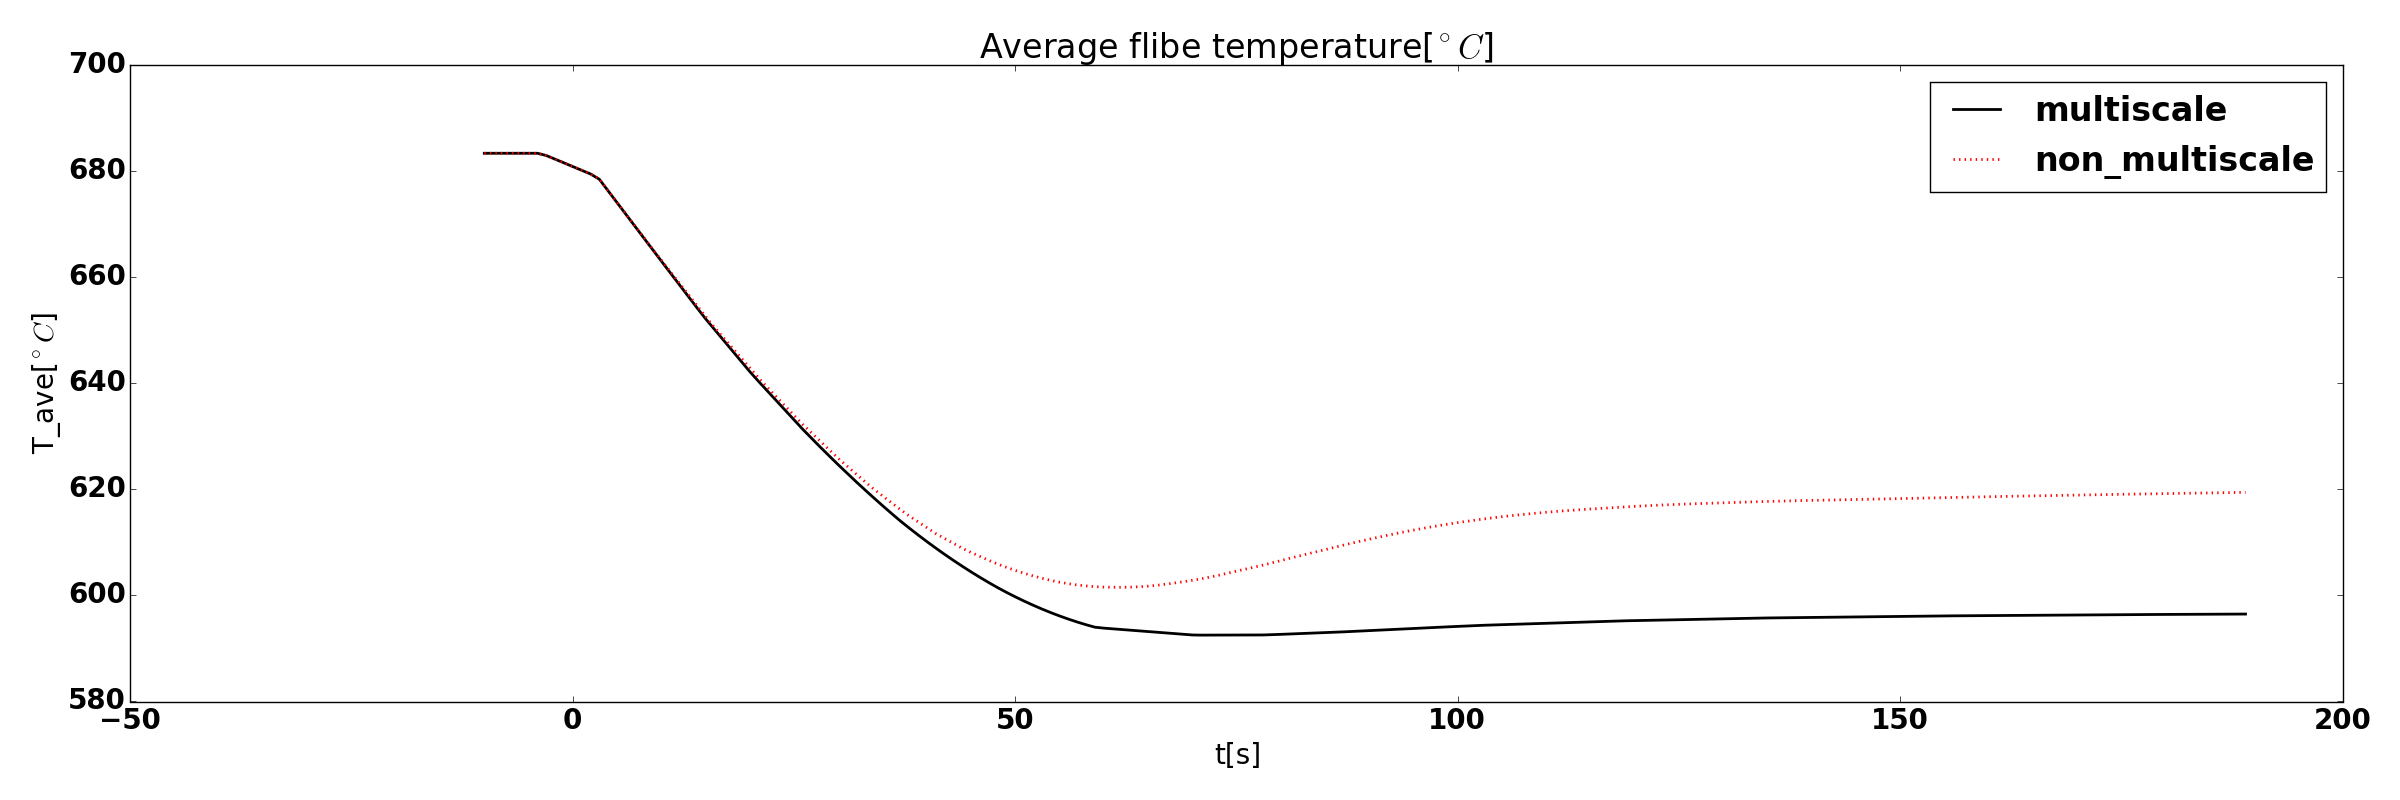
\includegraphics[width=1\textwidth]{./images/diffusion/tmsr/OC/compare_multiscale/T_flibe_ave.png}
        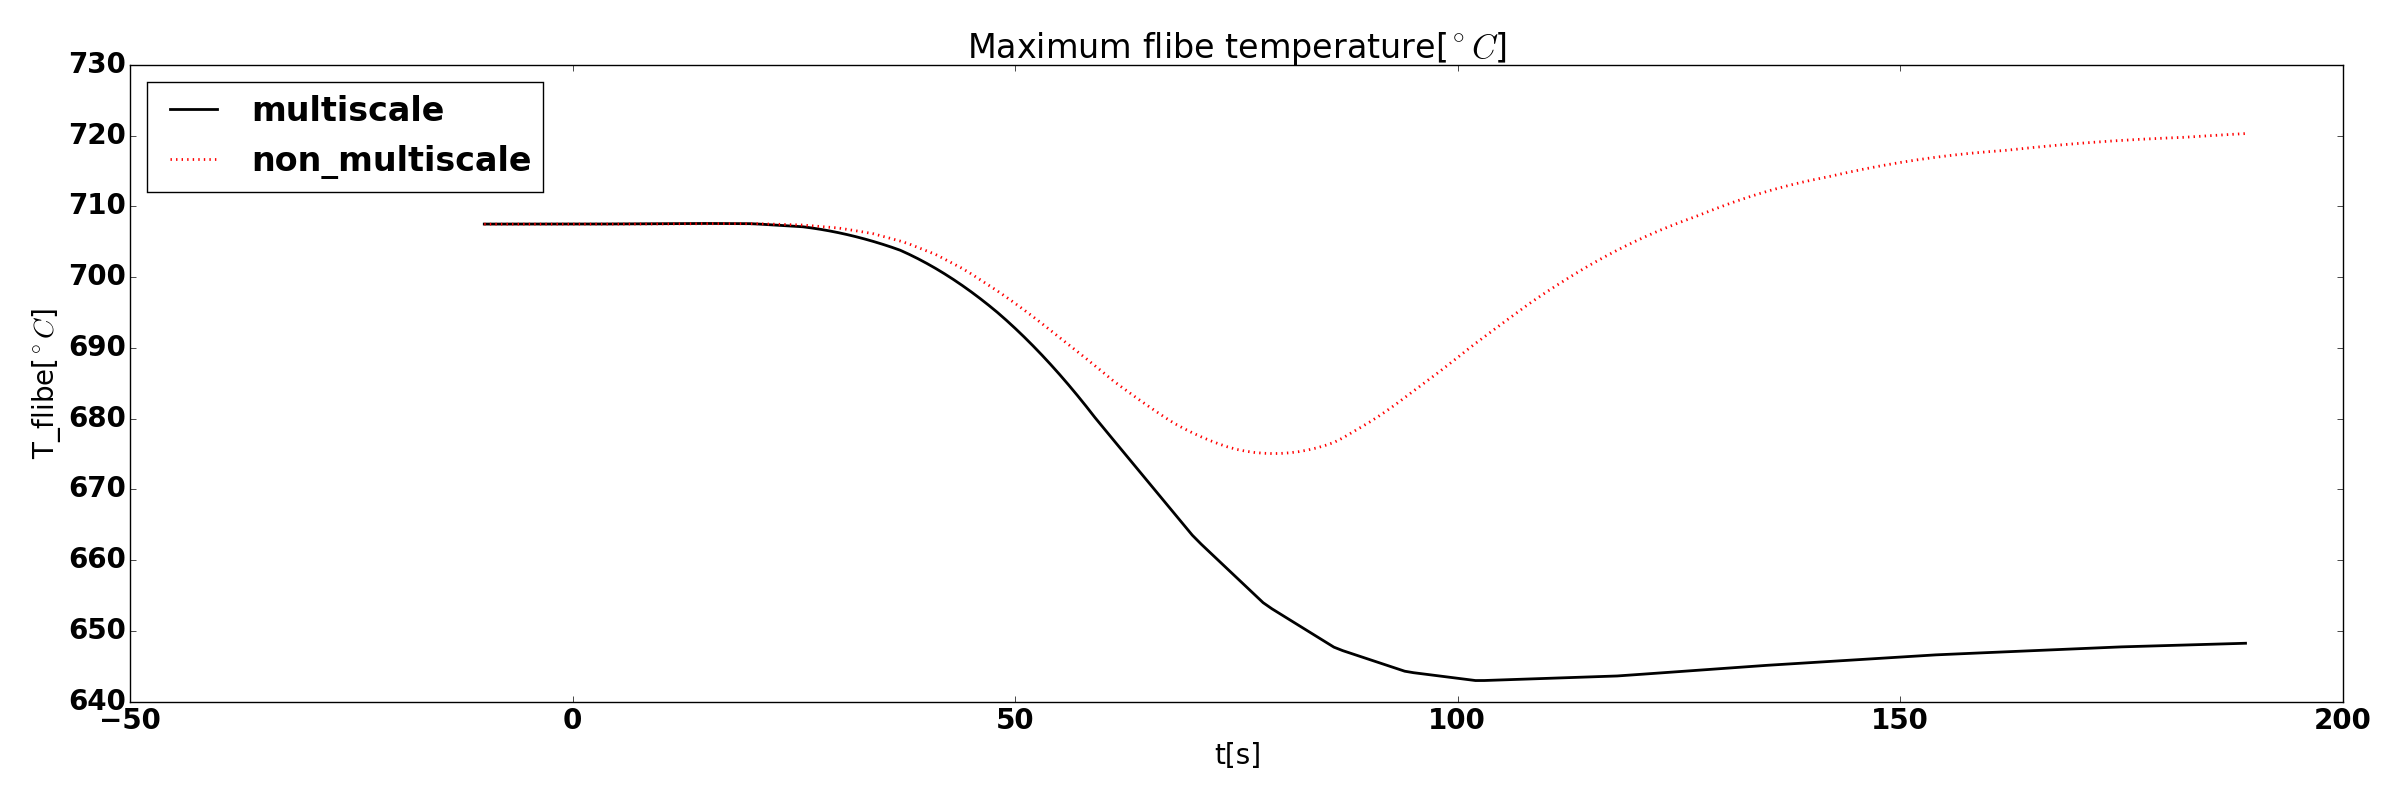
\includegraphics[width=1\textwidth]{./images/diffusion/tmsr/OC/compare_multiscale/T_flibe_max.png}
        \caption{Core maximum and average flibe temperature during overcooling transient}
        \label{fig:tmsr_oc_flibe}
\end{figure}


\begin{figure}[h]
    \centering
        
        \centering
        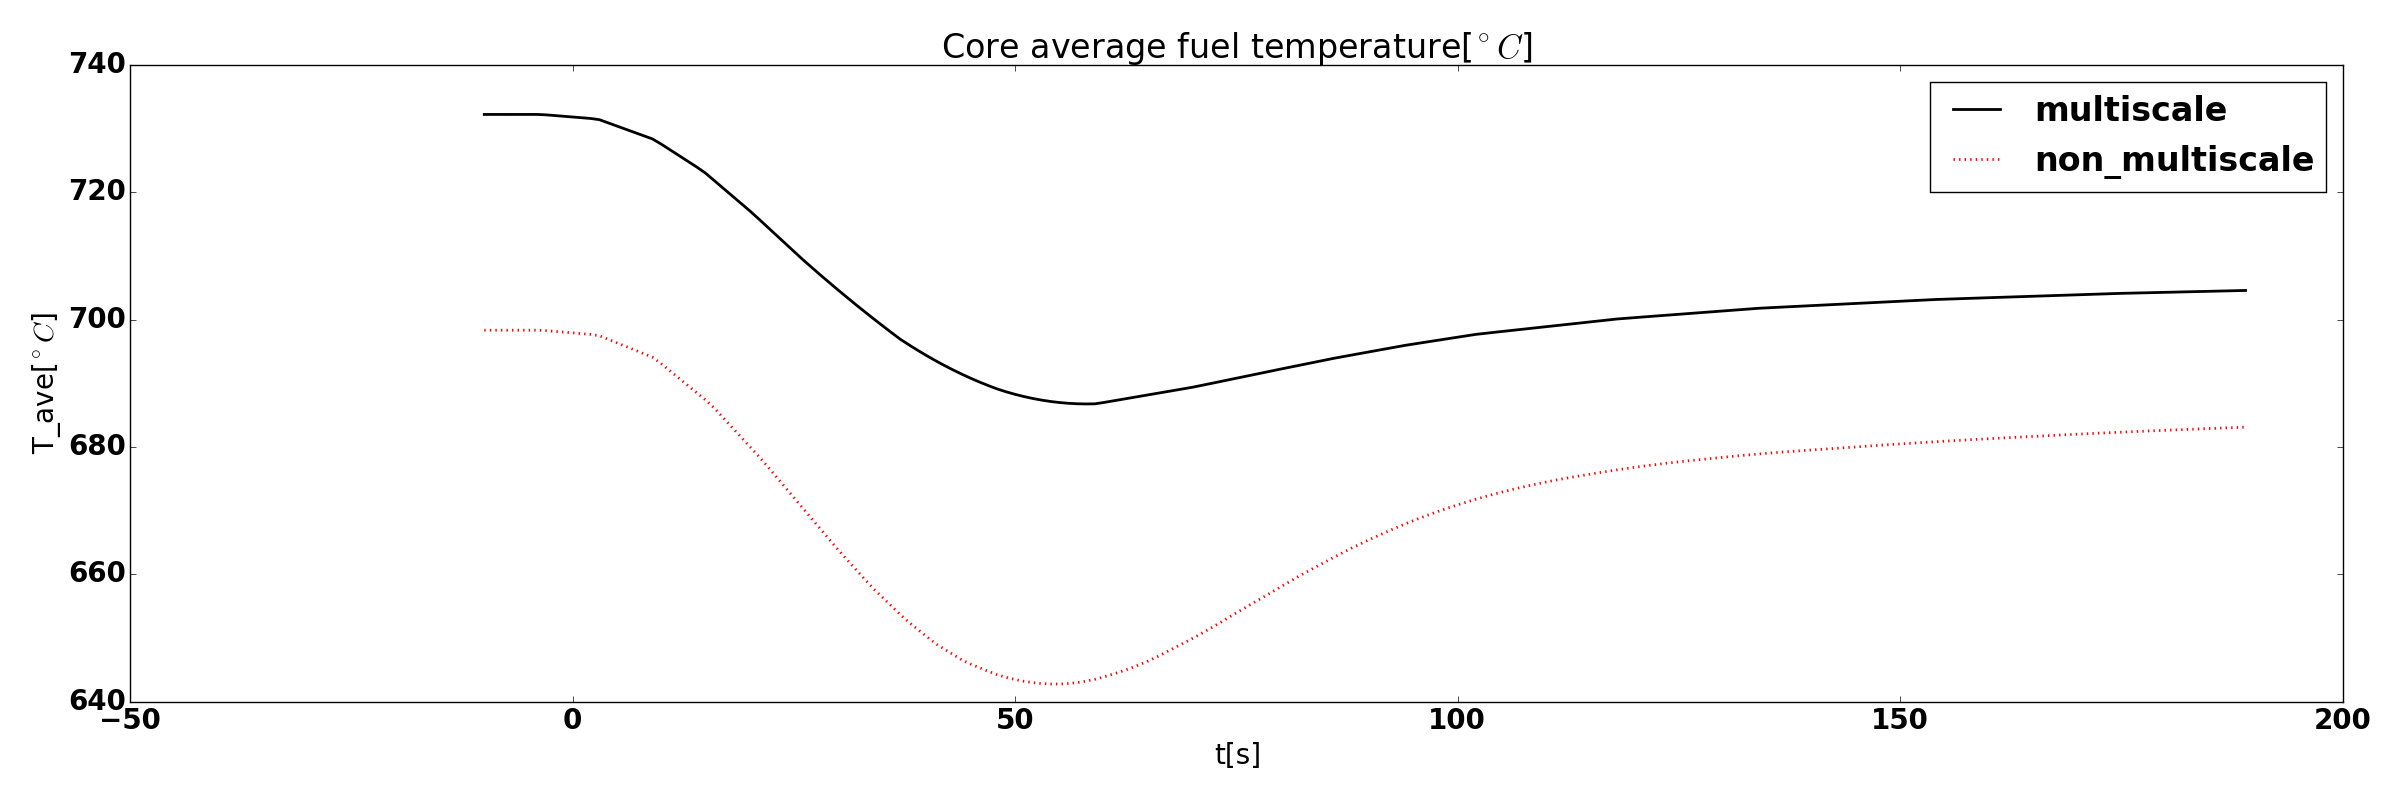
\includegraphics[width=1\textwidth]{./images/diffusion/tmsr/OC/compare_multiscale/T_fuel_ave.png}
        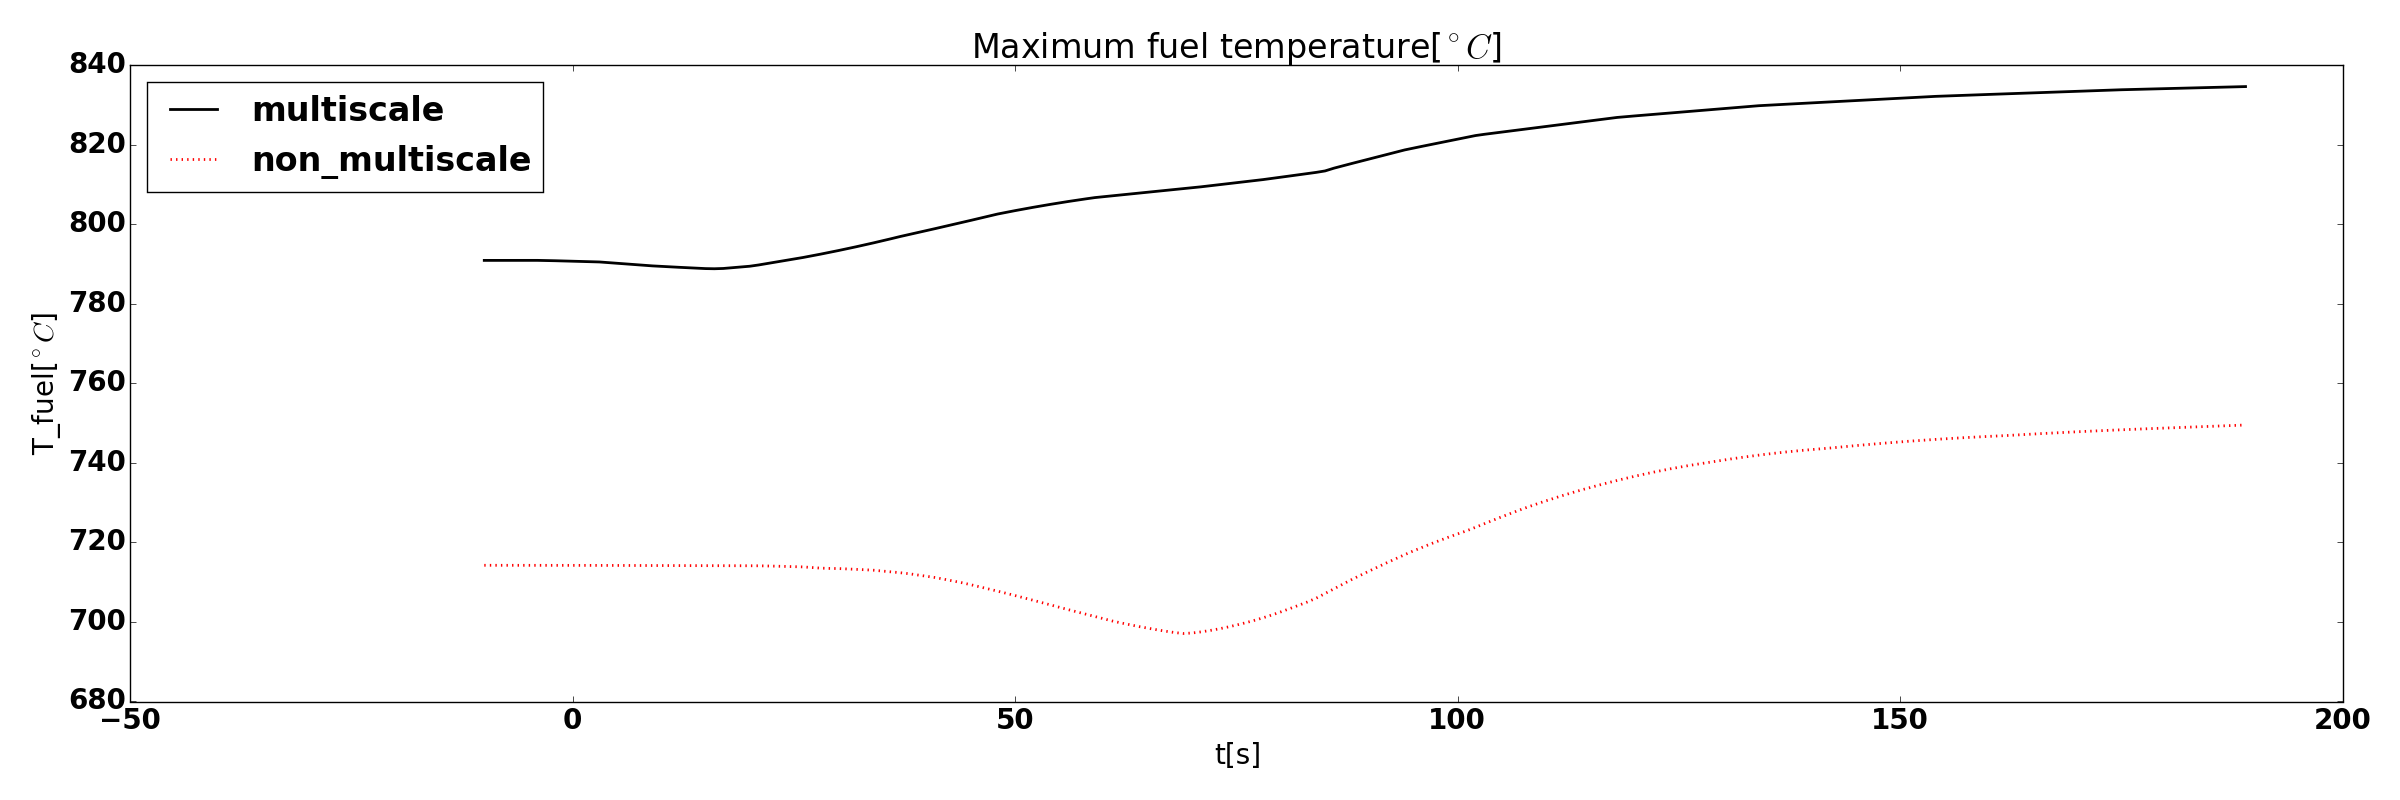
\includegraphics[width=1\textwidth]{./images/diffusion/tmsr/OC/compare_multiscale/T_fuel_max.png}

        \caption{Core average and maximum fuel temperature during overcooling transient}
        \label{fig:tmsr_oc_fuel}
\end{figure}


\begin{figure}
    \centering
    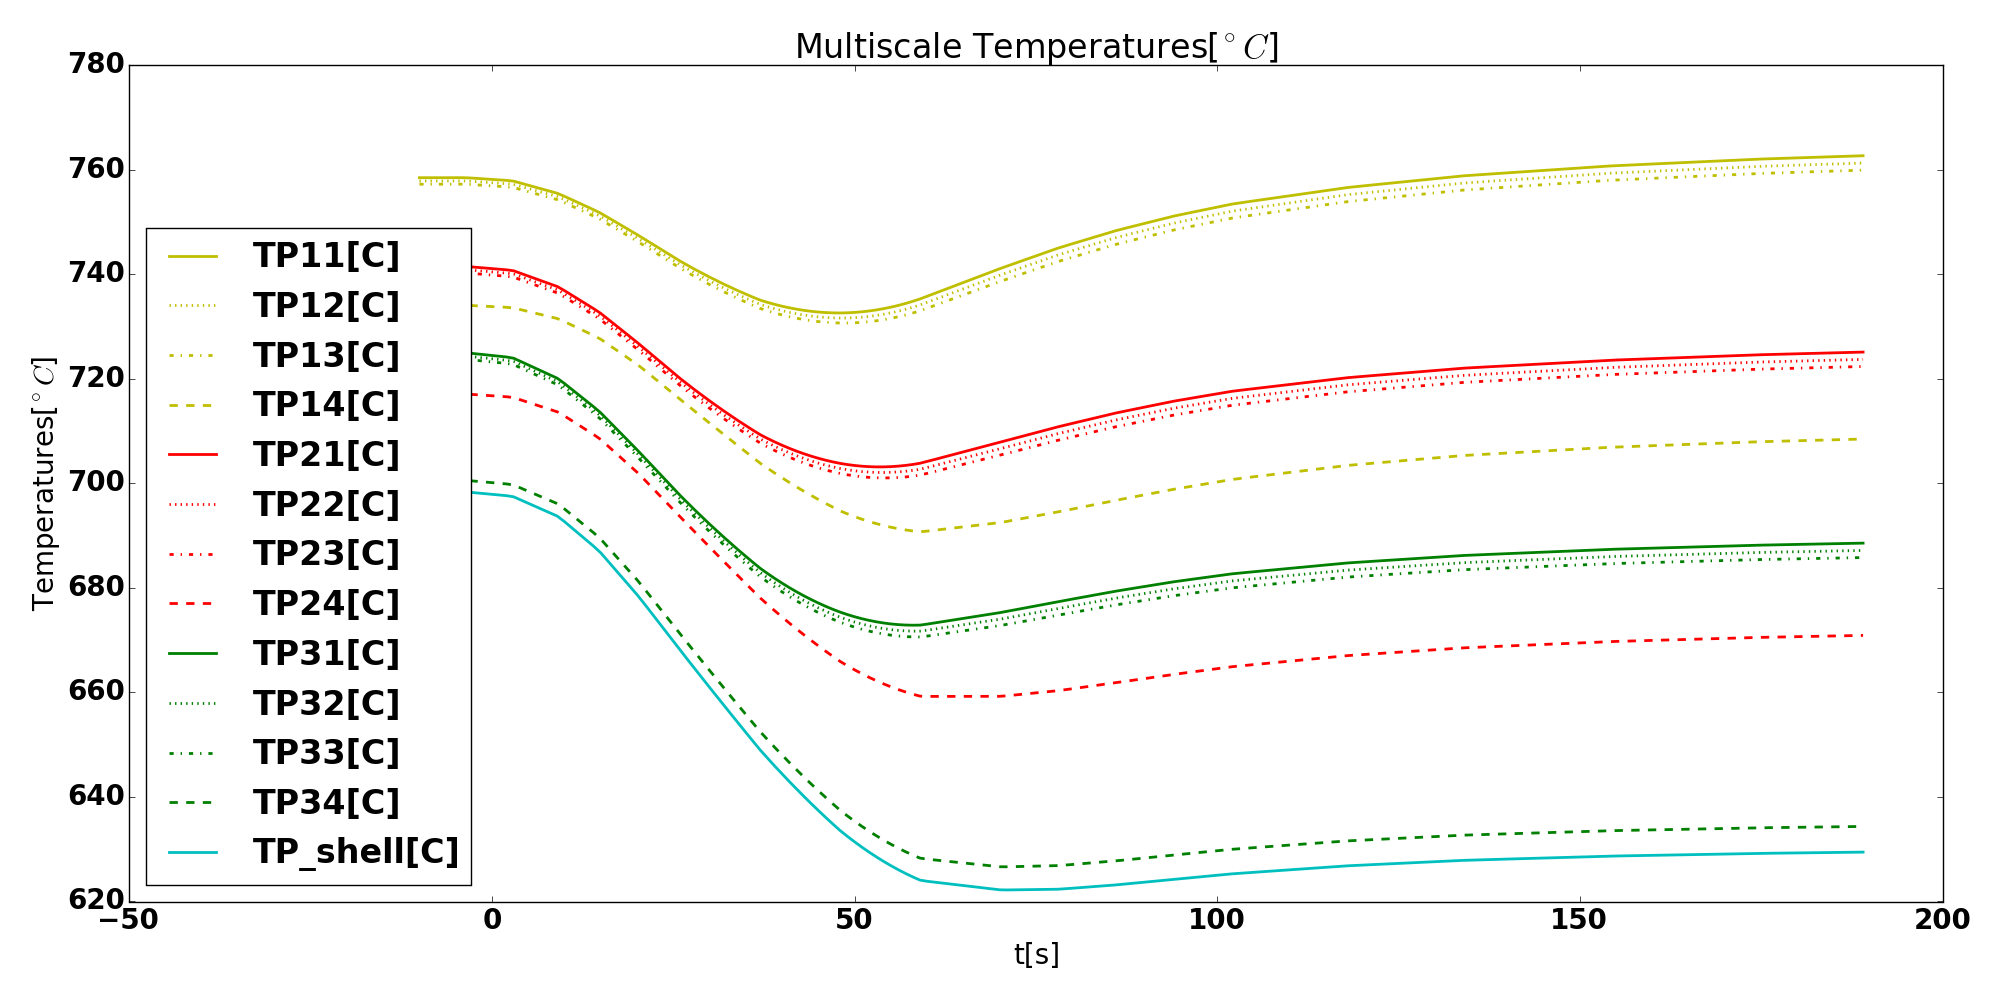
\includegraphics[width=\textwidth]{images/diffusion/tmsr/OC/compare_multiscale/temps.png}
    \caption{Core average of temperatures inside fuel pebbles during overcooling transient for TMSR SF-1. Notation for temperatures: $TP_{ij}$ represents the ith TRISO layer in the jth pebble layer. $TP_{shelll}$ is the temperature in the graphite shell of the pebble.}
    \label{fig:temps_OC_tmsr}
\end{figure}


Starting from the steady state conditions (section \ref{sec:TMSR_SS}), the inlet coolant temperature is decreased by 100$^{\circ}C$ in 10 seconds and remains at the lower level during the simulated overcooling transient. Within the short timescale of the simulation, it is reasonable to assume that the other inlet conditions (e.g. coolant mass flow rate) and the reactor control parameters (e.g. control rod positions) remain unchanged. 

The colder coolant introduces positive reactivity insertion due to negative flibe temperature reactivity feedback, which causes a power increase, as shown in figure \ref{fig:OC_power}. The increase is slow at the beginning because the temperature reactivity feedback is mainly from the coolant, weaker then the Doppler feedback from the fuel, which comes into effect after about 10 seconds when the cooling reaches the fuel materials. 
Because the transient is initiated in the coolant, the multiscale power increases less than that in the model with uniform fuel temperature, because it can capture the feedback from fuel while the fuel material gets cooled gradually from the shell to the center kernel.
The change in temperature in turn results in  negative reactivity feedback that stabilize the power at a higher level than the initial rate. 

Figure \ref{fig:tmsr_oc_flibe} shows that both the average and maximum coolant temperature drops at first due to the colder inlet and increase later due to the increased power.
The average coolant temperature drops immediately due to the decreased inlet temperature. 
On the other hand, the maximum coolant temperature, which is also the outlet temperature, is not affected until the colder coolant arrives at the top of the core. This parameter is directly related to the hot-leg temperature and determines the reactor safety margin. However, this is not a safety concern for over-cooling transients where the coolant temperature is below the steady state condition. 

Figure \ref{fig:tmsr_oc_fuel} shows the variation of both the maximum and the average fuel temperature during the transient, with two different models.
The average fuel temperature drops with the coolant, heats up from the reactivity feedback and in the end stabilizes at a lower level than the steady state temperature.
The location where the fuel temperature peaks changes from the center of the core to the top as the coolant flows through the core. At the end of the transient, the peak fuel temperature is higher than the steady state temperature despite the colder coolant that flows through the core, but is still well below the safety limit. 
Both the average and the maximum fuel temperature in the core is higher with the multiscale treatment, because it captures the feedback from the fuel correctly. 

Overall, the end state of the fuel temperature is lower while the coolant temperature is higher in the non-multiscale model because it overestimates the contribution to the negative reactivity feedback from the coolant. 
In fact, the estimated maximum flibe temperature in this case is much higher than in the multiscale case, even higher than the steady state value. This may lead to over conservatism in the design. 


If we take a closer look at the temperature profile inside the fuel pebbles during the transient, figure \ref{fig:temps_OC_tmsr} shows the temperature in each solid layer at each time stamp.
It takes a few seconds for the drop in the inlet coolant temperature to affect the solid temperature. The core-wise average temperatures in the fuel elements decrease at first as the cold coolant flows upward in the core.
At around 50 second, the temperatures increase due to the surge in power. The temperatures finally stabilize after about 150 seconds. The surface temperature is much lower than the steady state temperature because the coolant temperature is much lower.
The temperatures gradient inside a fuel pebble is higher after the transient because the power is at a higher level. The difference between the hottest layer and the shell changed from 60 K to 130 K after the transient. As a result, the inner most layer has a slightly higher temperature after the transients, although the safety margin to fuel damage is still very large. 


\section{Conclusion}
Strict safety requirement for next-generation reactors along with the progress in computer technology prompts the development, qualification and application of time-dependent multi-physics models for FHRs.
In this paper, a methodology for building coupled neutronics/thermal-hydraulics model for FHRs is described. It utilizes COMSOL Multiphysics to solve for neutron diffusion, delayed neutron precursor concentration equations and porous media CFD. Benchmarking with the Monte Carlo based model shows satisfying agreement. The model provides high resolution two dimensional or three dimensional results within a reasonable amount of time on a computer with 16.0 GB RAM and four Intel Core equipped with i7-4790K CPU at 4.00 GHz.

The Fick's law assumption in diffusion models does not take directional variations in neutron transport into account, and this assumption is violated in strong absorbers such as control rods. Furthermore, $SP_N$ treatment can be used in regions where the diffusion assumption is questioned, such as in the vicinity of the control rods.
This section describes a control rods modeling method based on the $SP_3$ approximation of NTE that is more accurate than the diffusion approximation, especially in control rod regions, and yet is considerably less expensive than the discrete ordinates ($S_N$) or spherical harmonics ($P_N$) approaches. In addition, the $SP_3$ equations can be solved in the same manner as the diffusion equations, which allows similar implementations with the same tools.

In conventional porous media formulation, only an average temperature inside the solid phase is computed. This is a reasonable assumption in steady state cases and in most slow transient problems where the fuel kernel temperature is very close to the temperature of the surrounding graphite matrix. However, in the case of fast transients involving large power excursions, the difference between fuel and graphite temperatures can be significant. Thus a detailed temperature profile inside the fuel pebbles and TRISO fuel kernels is necessary for accurately computing temperature, which is important in capturing the Doppler temperature reactivity feedback.
Overall, the power excursion in response to either a large reactivity insertion or a overcooling transient is dampened when a temperature profile in the fuel element is used, because the temperature reactivity feedback is captured more realistically at the place where the largest feedback occurs. 


Although the results discussed in this paper are based on a specific FHR design - the TMSR, the methodology can be used for all pebble bed FHRs.

Steady state and transient results of power, temperatures and neutron flux are discussed in this paper. The use of thermal resistant TRISO fuel, flibe coolant and graphite reflectors renders the core extremely robust against accidents. 
Because of the use of highly robust elements in the core, failures due to high temperature would be more likely to occur at the hot legs outside the core.
The fuel and coolant temperature during a 1\$ reactivity insertion is within the safety limit.
Likely, during the overcooling transient, where the coolant inlet temperature is dropped by 100 $^{\circ}C$ in 10 seconds, the core-wise maximum fuel temperature is 950 $^{\circ}C$, largely below the safety limit for fuel element. The coolant temperature stabilizes at a lower level than the initial condition, but is still above the salt freezing point.


\section*{References}

\bibliography{references}

\end{document}
